\documentclass[review]{elsarticle}

\usepackage{achinDefs}
\usepackage{lineno,hyperref}
\modulolinenumbers[5]

\journal{Journal of \LaTeX\ Templates}


\begin{document}

\begin{frontmatter}

\title{Data Predictive Control: Theory and Applications\tnoteref{mytitlenote}}
\tnotetext[mytitlenote]{The research leading to these results has received funding from the Italian Government under Cipe resolution n.135 (Dec. 21, 2012), project \emph{INnovating City Planning through Information and Communication Technologies} (INCIPICT).}

\author[FSaddress,EC]{Francesco Smarra\corref{mycorrespondingauthor}}
\cortext[mycorrespondingauthor]{Corresponding author}
\ead{francesco.smarra@univaq.it@univaq.it}

\author[AJaddress,EC]{Achin Jain}
\ead{achinj@seas.unpenn.edu}
\author[TDRaddress,EC]{Tullio de Rubeis}
\ead{tullio.derubeis@graduate.univaq.it}
\author[TDRaddress]{Dario Ambrosini}
\ead{dario.ambrosini@ing.univaq.it}
\author[FSaddress]{Alessandro D'Innocenzo}
\ead{alessandro.dinnocenzo@univaq.it}
\author[AJaddress]{Rahul Mangharam}
\ead{rahulm@seas.upenn.edu}

\address[FSaddress]{Department of Information Engineering, Computer Science and Mathematics, Universit\`{a} degli Studi dell'Aquila, L'Aquila, Italy}
\address[AJaddress]{Department of Electrical and Systems Engineering, University of Pennsylvania, Philadelphia, USA}
\address[TDRaddress]{Department of Industrial and Information Engineering and Economics, Universit\`{a} degli Studi dell'Aquila, L'Aquila, Italy}
\address[EC]{Equal contribution}

%% ABSTRACT
\begin{abstract}
Model-based control techniques have been widely used over the past years in control systems to improve system performance of simple controllers, such as PID, bang-bang, etc. Among these, one of the most popular is Model Predictive Control (MPC) due to its ability to predict the system's behavior over a future horizon and handle constraints in the optimal control setup. A key factor prohibiting the widespread adoption of MPC for complex systems is related to the difficulties (cost, time, and effort) associated with the model identification. On the other hand, data-driven models are not suitable for control because of non-physical models. We introduce a novel idea for predictive control based on system data, Data Predictive Control (DPC), leveraging machine learning algorithms, in particular regression trees and random forests. Using a bilinear model, we show that DPC has comparable performance with MPC. We further apply DPC to the Demand Response problem of a large scale multi-story EnergyPlus building building model, and show that DPC curtails the desired power usage with high confidence. Finally, we use DPC to optimize ON/OFF scheduling of the heating system of a real house in order to minimize the power consumption while guaranteeing thermal comfort for occupants. Our results show that with DPC we obtain an energy saving in terms of primary energy up to $49.2\%$ when compared to a bang-bang controller.
\end{abstract}

\begin{keyword}
Energy efficiency, demand response, predictive control, machine learning
\end{keyword}

\end{frontmatter}


%% SECTIONS
\section{INTRODUCTION}
\label{S:intro}

\textcolor[rgb]{0,0,1}{Control-oriented predictive models of an energy system's dynamics and energy consumption, are needed for understanding and improving the overall energy efficiency and operating costs of a building.
With a reasonably accurate forecast of future weather and building operating conditions, dynamical models can be used to predict the energy needs of the building over a prediction horizon, as is the case with Model Predictive Control (MPC) \cite{Sturzenegger2016}.
However, a major challenge with MPC is in accurately modeling the dynamics of the underlying physical system.
The task is much more complicated and time consuming in the case of a large building and often times, it can be even more complex and involved than the controller design itself.
After several years of work on using first principles based models for peak power reduction, energy optimization and thermal comfort for buildings, multiple authors~\cite{Sturzenegger2016, vzavcekova2014} have concluded that the biggest hurdle to mass adoption of intelligent building control is the cost, time and effort required to capture accurate dynamical models of the buildings.
The user expertise, time, and associated sensor costs required to develop a model of a single building is very high. Thus, the payback period for the upfront hardware and software installation is expected to be too high, making MPC an uneconomical choice for energy management.}

\textcolor[rgb]{0,0,1}{Why is physics-based modeling hard for complex systems like buildings or what are the reasons of such modeling complexities?}
\begin{enumerate}
	\item \textcolor[rgb]{0,0,1}{\textbf{Model capture} - a building modeling domain expert typically uses a software tool to create the geometry of a building from the building design and equipment layout plans, add detailed information about material properties, about equipment and operational schedules. There is always a gap between the modeled and the real building and the domain expert must then manually tune the model to match the measured data from the building~\cite{New2012}. 
	Moreover, the modeling process also varies from building to building with the construction and types of installed equipment.
	Another major downside with physics-based modeling is that enough data is not easily available and guesses for parameter values have to be made, which also requires expert know-how.
	\item \textbf{Change in model properties over time} - even if the model is identified once via an expensive route as in \cite{Sturzenegger2016}, as the model changes with time, the system identification must be repeated to update the model. Thus, model adaptability or adaptive control is desirable for such systems.
	\item \textbf{Model heterogeneity} further prohibits the use of model-based control. For example, unlike the automobile or the aircraft industry, each building is designed and used in a different way. Therefore, this modeling process must be repeated for every new building. }
\end{enumerate}

\textcolor[rgb]{0,0,1}{Due to aforementioned reasons, the control strategies in such systems are often limited to fixed, sometimes ad-hoc, rules that are based on best practices. 
The alternative is to use black-box, or completely data-driven modeling approaches, to obtain a realization of the system's input-output behavior. 
The primary advantage of using data-driven methods is that it has the potential to eliminate the time and effort required to build white and grey box building models. 
Listening to real-time data, from existing systems and interfaces, is far cheaper than unleashing hoards of on-site engineers to physically measure and model the building. Improved building technology and better sensing is fundamentally redefining the opportunities around smart buildings. 
Unprecedented amounts of data from millions of smart meters and thermostats installed in recent years has opened the door for systems engineers and data scientists to analyze and use the insights that data can provide, about the dynamics and power consumption patterns of these systems. }

\textcolor[rgb]{0,0,1}{The key question now is: can we employ data-driven techniques to reduce the cost of modeling, and still exploit the benefits that MPC has to offer?
We therefore look for automatic data-driven approaches to control, that are also adaptive, scalable and interpretable.
We solve this problem by bridging Machine Learning and Predictive Control. In particular, in this paper, we present a method based on Random Forests which uses historical data for receding horizon control.}

\textcolor[rgb]{0,0,1}{
Next, we present an example to illustrate how data-driven modeling reduces the cost of modeling buildings. 
}

%\paragraph{Example} \textcolor[rgb]{0.00,0.00,1.00}{As a first} example of such modeling complexity, consider the grey-box approach in \cite{Braun2002}. The scope of such approach is to predict the heat transfer rate to the air within the building. In particular, the authors addressed a single zone modeling problem using an equivalent $RC$ model. To this end, five different types of structures are considered in the example: external walls, ceiling/roof, floor, internal walls and windows. Each of these elements are represented using $3$ resistances, $2$ capacitances and $2$ temperatures, except for the windows that are represented only with resistances since they have a negligible energy storage. A model consisting of $8$ states and $9$ inputs, including disturbances such as solar radiation and others, with the instantaneous heat gain to the building air from all surfaces as output, is created for the zone. To have a complete LTI model, $9$ parameters are needed to be estimated via a non-trivial training process, using a collection of information associated with a physical description of the building (see \cite{Braun2002} for more details). Extending this result, for the building we consider in Section \ref{S:realCaseStudy} with $10$ different zones, we would need to consider a model with approximately $80$ states and $90$ parameters to be estimated.

\subsection{Example for comparison of modeling complexity: physics-based vs data-driven}
\textcolor[rgb]{0,0,1}{In this section, we provide a detailed example that describes the difference in terms of complexity when we model a building using physical laws and machine learning.
We show that the data-driven modeling eliminates several drawbacks that occur using physics-based models such as the need to have very good knowledge of the building structure and the material properties, time required to build a model, and limited availability of sensor measurements.}

\textcolor[rgb]{0,0,1}{The building under consideration is taken from \cite{Sturzenegger2016}. It is located in Allschwil, Switzerland. It has 6 floors of which only the second floor is modeled, and is assumed to represent all other floors. The total air conditioned floor area is $6000\ \mathrm{m^2}$ ca.}

\subsubsection{Physics-based modeling}
\label{SSS:physics-based}
\textcolor[rgb]{0,0,1}{We describe the physics-based approach based on an RC network outlined in \cite{Sturzenegger2016}.
The building is modeled as a bilinear system constructed from physical principles.
The modeling process consists of three steps:
\begin{enumerate}
	\item Building geometry and construction data are used together with first-principles to derive the following linear model for the building's thermal dynamics:
		\begin{equation}\label{E:RCZoneEq}
			\dot x(t) = A_x x(t) + B_q q(t).
		\end{equation}
		This model describes the behavior of the zone, wall, floor and ceiling temperatures.
		Walls, floors and ceilings are considered as divided into layers with different features. Therefore, each zone was described with an RC network model (see Figure 3-10 in \cite{SturzeneggerTR}), where the capacitances represent the states of the layers and the resistances represent the thermal resistance of the layers.
%		\begin{figure}[t]
%			\begin{center}
%				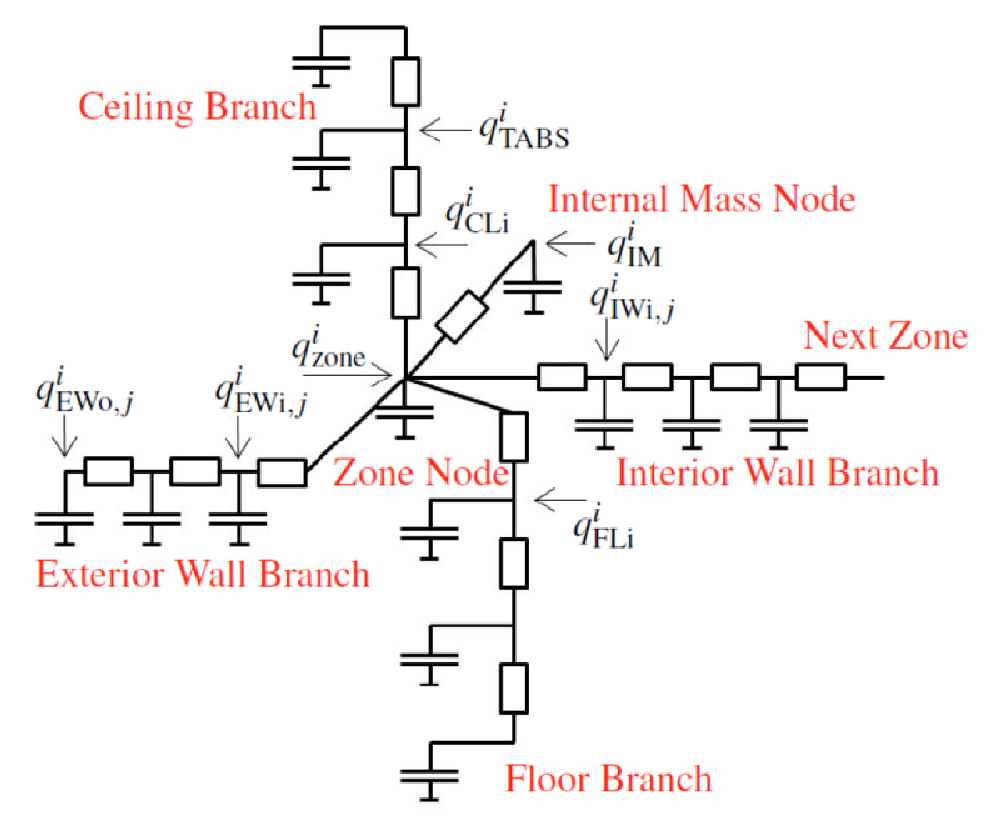
\includegraphics[width=0.6\textwidth]{figures/RC_net.eps}
%				\caption{RC model of a zone. $q$ represents the external heat fluxes}\label{F:RCnet}
%			\end{center}
%		\end{figure}
		The heat exchange between two adjacent layers, i.e. layer ``a" and layer ``b", is modeled to be proportional to the temperature difference of the two layers and the corresponding thermal resistance $R$ given by
		\begin{equation}\label{E:RCHeatExchange}
			\begin{aligned}
				&C_a\dot x_a = \frac{x_b(t) - x_a(t)}{R},\\
				&C_b\dot x_b =  \frac{x_a(t) - x_b(t)}{R},
			\end{aligned}
		\end{equation}
		where $C_a$ and $C_b$ are the heat capacitances of the layers. This is done for each layer of each zone, obtaining the compact representation given in \eqref{E:RCZoneEq}. The thermal parameters are derived from zones geometry and material properties.
	\item External heat fluxes, modeled as a bilinear model, affect the building directly as well as indirectly through zones:
		\begin{equation}\label{E:RCfluxes}
			q(t) = A_q x(t) + B_{q,u}u(t) + B_{q,d}d(t) + \sum_{i=1}^{n_u}{[\left(B_{q,du,i}d(t) + D_{q,xu,i}x(t)\right)u_i(t)]},
		\end{equation}
		where $u$ are the inputs and $d$ the disturbances of the system.
%		Equation \eqref{E:RCfluxes} comes from a series of 20 equations analyzed in Section 3.3.1.3 of the Technical Report \cite{SturzeneggerTR}, that we do not report here for the sake of simplicity. 
Equation \eqref{E:RCfluxes} for the heat flux is obtained by modeling
	\begin{enumerate}
		\item heat exchange associated with the building hull (except for windows), both conductive and radiative part,
		\item  heat flux to each thermally activated building system (TABS), i.e. pipes buried in the concrete slabs of the floors carrying hot/cold water,
		\item heat flux through the windows in three different parts: radiation due to elements directly in contact with the zone air, conduction through the window, and absorption of the solar radiation through the window,
		\item convection due to internal gains due to occupants, appliances and lighting, and
		\item the effects of the AHU.
	\end{enumerate}
	\item The resulting system \eqref{E:RCZoneEq} is discretized with a sampling time of $15\ \mathrm{min}$.
	This model has approximately 300 states that include temperature of the zones, walls and floors on the second floor.
	The outputs of the system are the zone temperatures.
	Since the performance of the state estimation, that is needed to compute the optimal control inputs using MPC depends on the number of states, an approximated model with fewer states is needed.
	To this aim, different averaged temperatures of the building facades (North, South, West, East) and the zones are considered, obtaining an approximated model with 35 states.
	This  approximate model is then considered ``suitable for MPC" (see Section 3.3.1.4 in \cite{SturzeneggerTR}). 
\end{enumerate}}
	
\textcolor[rgb]{0,0,1}{In summary, the approximate model has the following state, input and disturbance variables:
	\begin{itemize}
		\item 5 outputs: averaged room temperature for each group of zones (North, South, West, East, Center). The rooms are equipped with temperature sensors.
		\item 18 inputs: TABS heating heat flux, TABS cooling heat flux, averaged transmitted solar heat flux for each group of zones (North, South, West, East) that is estimated using blinds position measurements, air massflow through the energy recovering mode, air massflow bypassing the energy recovering mode, air massflow through the air cooler, AHU heat coil heat flux, lighting power for the offices for each group of zones (North, South, West, East), and radiator heat flux in the corner offices (North, South, West, East).
		\item 7 disturbances: internal gains in the offices and internal gains in non-office zones, which are predicted using a standard schedule, ambient temperature and solar radiation on facade (North, South, West, East) whose values were obtained through Kalman filtering using measurements from the weather station placed on the roof of the building. This filtering is needed to take into account the shadowing of the neighboring buildings.
	\end{itemize}
An EnergyPlus model is built for this system, and model parameters of matrices $A_x$, $B_q$, $A_q$, $B_{q,u}$, $B_{q,d}$, $B_{q,du,i}$, $D_{q,xu,i}$ in Equations \eqref{E:RCZoneEq} and \eqref{E:RCHeatExchange} are derived using geometry and materials data from the EnergyPlus model.
This was a choice of the authors; real geometry and materials data can also be used to estimate the model parameters, if necessary data are available. 
For this particular building, 24 parameters are estimated/taken form a datasheet/computed for the considered zone model.
Although some of the parameters are in common between different zones, the others are found independently for each zone.
To simplify, the parameters of all the other floors are assumed to be identical which is not true in reality.
To derive the EnergyPlus model using the available measurements and to use the same control implemented in the building, the EnergyPlus model is coupled with MATLAB using BCVTB \cite{Wetter2015}.
}
%To identify the model a total of 294 MATLAB signals were sent to the EnergyPlus model and a total of 1081 EnergyPlus signals were sent back to Matlab.

\textcolor[rgb]{0,0,1}{The physics-based approach, although detailed and accurate (in some cases), is cost and time prohibitive. The long and complex modeling procedure that is unique to every building poses practical challenges in applying MPC to large scale buildings.}

\subsubsection{Data-driven modeling}
\textcolor[rgb]{0,0,1}{The data-driven approach we propose, on the other hand, ignores the physical details of the building operation. Instead, we use machine learning to learn black-box models where our objective is to find the hyperparameters (for a given structure like Random Forests) of a model that best explains the input-output relationship.}

\textcolor[rgb]{0,0,1}{The goal with the data-driven modeling is to learn a function map
\begin{equation}
\label{E:MLexample}
y(t) = f(u(t),\dots,u(t-\delta_u), d(t),\dots, d(t-\delta_d)),
\end{equation}
where \(y\) represents the outputs, \(u\) the inputs and \(d\) the disturbances as defined earlier, and \(\delta\) is a lag variable.}

\textcolor[rgb]{0,0,1}{The data-driven modeling in the case of buildings has several advantages over the physical counterpart.}
\begin{enumerate}
	
	\item \textcolor[rgb]{0,0,1}{\textbf{Domain expertise:} 
	This procedure (\textcolor[rgb]{1,0,0}{NOT CLEAR IF EXPLAINED IN ONLY 2 LINES BEFORE}) eliminates the need of a building expert, simplifies the modeling complexities (\textcolor[rgb]{1,0,0}{HOW?}) described in Section \ref{SSS:physics-based} which ultimately reduces the cost of modeling a building. Further, for a new building, given the historical data from the building, the same process can be repeated to identify a control-oriented model for MPC.}
	
	\item \textcolor[rgb]{0,0,1}{\textbf{Sensor cost:}
	Due to large number of states and variables in the physical modeling, a lot of measurements are needed to use the model to predict the system's behavior \textcolor[rgb]{1,0,0}{IF USING A MODEL-BASED APPROACH}.
	This can be expensive due to necessary new sensor installations.
	Moreover, when some measurements are not directly available from the sensors, observers are needed for state estimations.
	However, observability problems can limit the construction of such observers \cite{Dorf2011MCS}. 
	On the other hand, data-driven modeling obviates the need to model the state of the walls and floor layers\textcolor[rgb]{1,0,0}{AND OTHER STATES DIFFICULT TO MEASURE} so we do not have as many states.\textcolor[rgb]{1,0,0}{EXPLAIN THAT THE MACHINE LEARNING ALGORITHM IS ABLE TO COMPENSATE MISSING VARIABLES}
	It relies only on direct measurements from the sensors such as thermostats and multimeters reducing the need for new installations and hence the cost of modeling.
	Further, when some of the states are not directly measurable, often adding proxy \textcolor[rgb]{1,0,0}{I.E. ??}variables suffices. 
	For example, if we do not have the measurement of the energy produced by a photovoltaic panel, the weather conditions will account for it.}
	
	\item \textcolor[rgb]{0,0,1}{\textbf{Linearity assumption:}
	If \(y\) in Equation \eqref{E:MLexample} is the average room temperature for one of the zones, a nonlinear function \(f\) is more appropriate, for example \(f\) may belong to the class of Neural Networks or Random Forests. 
	During physical modeling in \eqref{E:RCHeatExchange}, in order to keep the model simple, the heat exchange between layers is modeled with a linear behavior. 
	Hence all the nonlinearities were neglected.
	In the case of heat flux in \eqref{E:RCfluxes}, again, a linear model is not good enough to provide a good approximation. For this reason a bilinear model was considered.
	However, more complex nonlinearities have been neglected due to the already high complexity of the model \cite{Sturzenegger2016}. 
	In data-driven modeling, we can relax these linearity assumptions as nonlinear functions can be learned rather efficiently and accurately.\textcolor[rgb]{1,0,0}{IT IS NOT CLEAR THAT THE DD ALGORITHM TAKE CARE OF IT CREATING ITS INTERNAL STRUCTURE}}
	
	\item \textcolor[rgb]{0,0,1}{\textbf{Other assumptions:} 
	Due to the high modeling complexity, physical modeling neglects different geometries and different materials of the floors assuming they are the same for each floor which is never true in reality.
	In many cases, the details of construction layout and equipments are not even available so many parameters have to be guessed.
	Data-driven modeling depends on the sensor data directly. 
	Hence, such assumptions never arise.}
	
\end{enumerate}

\textcolor[rgb]{0,0,1}{To summarize, the data-driven modeling simplifies the modeling of buildings to a large extent, reduces the overall cost and time investment while avoiding the linear model assumptions that we make in standard physical modeling procedure. Unlike physical modeling, the parameters of the model (or hyperparamters) are automatically determined by the learning algorithm, the best settings determined by cross validation.}

\textcolor[rgb]{0,0,1}{However, the challenge lies in using such models for optimal predictive control, which is exactly the focus of this paper.
We demonstrate how the training algorithm for Random Forests can be modified to develop control oriented models that are suitable in the MPC framework.}

\textcolor[rgb]{0,0,1}{
\subsection{Related work}
A vast literature exists in building energy applications that deals with Demand Response, peak power reduction, energy saving, thermal comfort, and related topics.
All these approaches can be classified based on two characteristics:
\begin{enumerate}
	\item the type of system model:
		\begin{itemize}
			\item model-based, that we consider both "white-box" and "grey-box" approaches: \cite{Shakouri2017SCS,Li2014EB,Yoon2014EB,Li2016AE,Harb2016EB,Salakij2016EB,Li2016E,Li2016EB,Hou2013,Cecconi2017EB};
			\item data-based, that is the "black-box" approach, mainly done using Neural Networks: \cite{Safa2017SCS,Neto2008EB,Magnier2010BE,Candanedo2017EB,Ascione2017E,Cecconi2017EB,Li2016AE};
			\item simulation tool-based, such as EnergyPlus \cite{energyPlus} and TRNSYS \cite{trnsys2000}: \cite{Yin2016EB,Christantoni2016EB};
		\end{itemize}
	\item the purpose these models are created for:
		\begin{itemize}
			\item only model creation and identification: \cite{Safa2017SCS,Neto2008EB,Magnier2010BE,Li2014EB,Li2016AE,Harb2016EB,Li2016EB,Candanedo2017EB,Cecconi2017EB,Ascione2017E};
			\item model identification and control (typically Predictive Control): \cite{Shakouri2017SCS,Yoon2014EB,Yin2016EB,Salakij2016EB,Li2016E,Hu2017AE}.
		\end{itemize}
\end{enumerate}
These papers are summarizes in Table \ref{T:RelatedWork} highlighting the differences.
We also emphasize the case studies the results are applied to, and whether the authors use experimental data to simulate their algorithms.
Only in three cases the algorithms are tested on real systems (see Table: RI - Real Implementation).
We observe that except for the last 6 cases, which we discuss in detail, either model-based approaches or only tools are considered with/without control or data-driven modeling approaches without control.
%This is because bridging data-driven models with control theory, especially with the predictive control, introduces several issues \cite{Hou2013}.
Data-driven control has attracted increasing attraction in the recent years.
The last six papers of Table \ref{T:RelatedWork} that are more related to the methodology presented in this paper.
In particular, in \cite{Macarulla2017} the authors proposed a predictive control strategy based on Neural Networks, for boilers control in buildings, to decide the optimal time to switch-on the plan to guarantee energy saving and thermal comfort.
However, the approach is not easily scalable to different types of plants and does not use optimization in the closed-loop scheme.
In \cite{Costanzo2016} a reinforcement learning control strategy, called Model-Assisted Batch Reinforcement Learning, is considered to provide data-driven control for the demand response problem in HVAC systems.
Reinforcement Learning is a model-free methodology and is an alternative approach to MPC \cite{Ernst2009TSMC} (with pros and cons).
In \cite{Ferreira2012} the authors considered a data-driven predictive control based on Neural Networks to guarantee energy saving and  thermal comfort in public buildings.
Neural Networks are used in the closed-loop control scheme to determine a thermal comfort index based on parameters that can be measured or estimated, but no Neural Networks-based system state dynamics are included into the optimization problem.
%However, Neural Networks are a particular type of machine learning algorithm that provides complex nonlinear equations to describe the system's dynamics.
\cite{Afram2017} uses a Neural Network based data-driven state model as a plant simulator in the MPC closed-loop optimization.
More papers related to this topic can be found in the literature.
Unfortunately, since Neural Networks models are nonlinear, the MPC based on such models is also nonlinear.
This means that a global optimal solution can not be guaranteed. 
When the complexity of network is high, solving the optimization problem becomes harder due to nonlinearties.
To overcome this complexity, we introduced regression trees-based approach in \cite{Behl2016,Jain2017TCPS}.
In this paper, we provide a new methodology based on random forests, that overcome the drawbacks of our previous work.
It provides robustness with respect to disturbance uncertainties and has better performance when compared to other approaches (both optimal and rule-based).
In the next section, we emphasize the differences with our previous approaches.
}


\begin{table}[t!]
	\centering
	\textcolor[rgb]{0,0,1}{\small\begin{tabular}{llcccc}
		\toprule
		Ref.                             & Case study              & Exp.                & Tool                & MB/DD             & Control           \\ 
		\midrule
		\cite{Yin2016EB}                 & Commercial Building     & Yes                 & E+                  & None              & Yes               \\
		\cite{Christantoni2016EB}        & Commercial building     & Yes                 & E+                  & None              & Yes               \\
		\cite{Li2014EB}                  & Commercial building     & Yes                 & E+                  & MB                & No                \\
		\multirow{2}*{\cite{Harb2016EB}} & 2 office buildings and  &  \multirow{2}*{Yes} & \multirow{2}*{None} & \multirow{2}*{MB} & \multirow{2}*{No} \\
		                                 & 1 residential building  &                     &                     &                   &                   \\
		\cite{Li2016EB}                  & 2 commercial buildings  & n/a                 & E+                  & MB                & No                \\
		\cite{Shakouri2017SCS}           & Residential area        & No                  & None                & MB                & Yes               \\
		\cite{Yoon2014EB}                & 2 residential buildings & Yes                 & E+                  & MB                & Yes               \\
		\cite{Salakij2016EB}             & 3 residential buildings & No                  & E+                  & MB                & Yes               \\
		\cite{Li2016E}                   & 6 commercial buildings  & Yes                 & E+                  & MB                & Yes               \\
		\cite{Hu2017AE}                  & Residential building    & Yes                 & None                & MB                & Yes               \\
		\cite{Cecconi2017EB}             & Commercial building     & No                  & E+                  & MB-DD             & No                \\
		\cite{Li2016AE}                  & 2 commercial buildings  & Yes                 & E+                  & MB-DD             & No                \\
		\cite{Safa2017SCS}               & Office building         & Yes                 & None                & DD                & No                \\
		\cite{Neto2008EB}                & Office building         & Yes                 & E+                  & DD                & No                \\
		\cite{Magnier2010BE}             & Residential house       & Yes                 & TRANSYS             & DD                & No                \\
		\cite{Candanedo2017EB}           & Residential building    & Yes                 & None                & DD                & No                \\
		\cite{Ascione2017E}              & Office building         & No                  & E+                  & DD                & No                \\
		\cite{Macarulla2017}             & Commercial building     & Yes+RI              & None                & DD                & Yes               \\
		\cite{Costanzo2016}              & Living lab (1 room)     & Yes+RI              & None                & DD                & Yes               \\
		\cite{Ferreira2012}              & Commercial building     & Yes+RI              & None                & DD                & Yes               \\
		\cite{Afram2017}                 & Residential house       & Yes                 & None                & DD                & Yes               \\
		\cite{Behl2016}                  & 9 commercial buildings  & No                  & E+                  & DD                & Yes               \\
		\cite{Jain2017TCPS}              & Commercial building     & No                  & E+                  & DD                & Yes               \\
		\bottomrule
	\end{tabular}\normalsize}
	\caption{\textcolor[rgb]{0,0,1}{References ordered considering: case study they have been applied to; whether they used experimental data, other than simulated data, and if they did real implementation (RI), i.e. implemented the methodologies on real systems; if they used simulative tool; the type of the model considered, i.e. Model-Based or Data-Driven; if they used the model to do control.}}
	\captionsetup{justification=centering}
	\label{T:RelatedWork}
\end{table}


\textcolor[rgb]{0,0,1}{
\subsubsection{Previous work}\label{SSS:PreviousWork}
We highlight the differences with respect to our previous work.
\begin{itemize}
	\item In \cite{Behl2016} we use regression trees to setup an MPC problem and apply it to the problem of Demand-Response.
	However, these models can be used for optimal control with only one-step lookahead prediction.
	Hence, it is not possible to use such approach to control the system considering a prediction over an horizon of arbitrary length.
	\item This limitation is addressed in \cite{Jain2017TCPS}, where multi-output regression trees are used instead of single output trees.
	The different outputs correspond to different steps of the prediction horizon.
	This allows us to setup an MPC problem with a finite horizon.
	Modeling accuracy using single trees is strongly affected by overfitting and high variance.
	Such approach has the advantage to be extremely simple from the complexity point of view, but the range of applications is limited.
	\item In \cite{JainACC2017,JainCDC2017}, we take a different approach that improves the system's identification accuracy and robustness in MPC.
	Instead of considering a single tree/forest with multiple output, we consider multiple trees/forests with single output.
	Each tree/forest provides the prediction of the system's behavior for a different time step of the horizon.
	However, the results are based on simulated data and we did not account for inaccuracies in the weather forecast.
\end{itemize}
}

\subsection{Main contribution and paper organization}
%TO CLARIFY $\rightarrow$ \textcolor[rgb]{0,0,1}{Achin and Francesco}
%\begin{itemize}
%	\item Add more details
%	\item Emphasize difference between Section 4 and Section 5
%	\item Cite appendix
%\end{itemize}
%TO ADD $\rightarrow$ \textcolor[rgb]{1,0,0}{Tullio}
%\begin{itemize}
%	\item Add references for weather forecast accuracy
%	\item Quantify accuracy for short-term prediction for weather forcast to justify the assumption of perfect knowledge for the disturbance
%\end{itemize}
%TO ADD $\rightarrow$ \textcolor[rgb]{0,0,1}{Achin and Francesco}
%\begin{itemize}
%	\item Add subsection in Section 5 with simulation of DPC considering disturbance with added noise and show that we still have good performance
%\end{itemize}
In our previous work \cite{Behl2016,Jain2016,JainACC2017,JainCDC2017}, we introduced the concept of DPC for receding horizon control. In this paper, we extend these results providing the following contributions.
\begin{enumerate}
	\item In Section \ref{S:dpc}, we formally present the two following control techniques:
	\begin{enumerate}
		\item DPC with regression trees, and
		\item DPC with random forests.
	\end{enumerate}
	\item In Section \ref{S:proof}, we demonstrate the strength of DPC for receding horizon control via one-to-one comparison against a benchmark MPC controller using a bilinear building model whose parameters were identified using experiments on a building in Switzerland. We show that DPC captures 70\% variance in MPC and offers a comparable performance.
	\item Section \ref{S:casestudy} describes a practical application of DPC for Demand Response, where we apply DPC to a 6 story 22 zone building model in EnergyPlus \cite{Crawley2001} for which model-based control is not economical and practical due to extreme complexity. We show scalability and efficiency of DPC in providing financial incentives to the end-customers bypassing the need for high fidelity models. We observe that DPC provides the desired power reduction with an average error of 3\%.
	\item In Section \ref{S:realCaseStudy}, we implement DPC on the real data from an off-grid house located in L'Aquila (Italy), to find the optimal ON/OFF scheduling for the heating system in order to save energy while guaranteeing thermal comfort for the occupants. We quantify the total amount of energy saved, with respect to the classical bang-bang controller widely used in houses for temperature control, using an EnergyPlus model built specifically for the house. We show we can perform an energy saving that goes from $25.4\%$, if we guarantee thermal comfort, to $49.2\%$, if we allow very little discomfort in terms of rooms' temperature.
\end{enumerate}

\section{DATA PREDICTIVE CONTROL}

\label{S:dpc}



\textcolor[rgb]{0,0,1}{The central idea behind DPC is to obtain control-oriented models using machine learning on historical datasets of buildings and formulate the optimal control problem in a way that Receding Horizon Control (RHC) can be solved efficiently. Let an historical dataset $(\X,\Y)$ be given.
We define $\X = \{(x(k),u(k),d(k))\}_{k=1}^n$ the set of predictor variables (or features), i.e. the set of samples $(x(k),u(k),d(k))$ measured a time instants $k=1,\ldots,n$, where $x(k)\in\mathbb{R}^{n_x}$ is the vector of the \emph{measurable} state variables (e.g. the rooms temperatures and power consumption of the building), $u(k)\in\mathbb{R}^{n_u}$ is the vector of the \emph{measurable} input variables (e.g. the set-points and schedule information of the building) and $d(k)\in\mathbb{R}^{n_d}$ is the vector of the \emph{measurable and predictable} disturbance variables (e.g. weather historical data).
We define $\Y = \{y(k)\}_{k=1}^{n}$ the set of response variables, i.e. the set of measured samples $y(k)\in\mathbb{R}^{n_y}$ representing the variables we wish to predict with our model. In the most general case, when we want to predict all measured variables, the response variables are represented by the state variables at the next time step, i.e. $y(k) = x(k+1)$. However, in general, we only wish to predict a subset $y(k) = \bar x(k+1) \subset \mathbb{R}^{n_x}$ of variables, e.g. only room temperatures and power consumption.
Clearly, $|\X| = |\Y| = n$ is the number of time samples of the dataset.\\
We remark that, as explained in Section \ref{secModelingIssuesExample}, the dataset $(\X,\Y)$ does not contain non-measurable states such as temperature of wall layers, ceiling, floor, etc.: nevertheless, our simulated and experimental results show that our data-driven methodology is able to compensate the absence of such variables while providing excellent prediction accuracy.}



\textcolor[rgb]{0,0,1}{Our goal is to learn data-driven models, using Regression Trees and Random Forests, that relate the value of the response variables (possibly for a certain future time horizon) with the value of the predictor variables and can be used to set up an MPC problem. To this aim, in the simplest example of one time-step prediction, we need to derive a model with a closed-form expression of the following form
\begin{equation}\label{E:GenericModel}
	y(k)=x(k+1)=f(x(k),u(k),d(k)).
\end{equation}
However classical Regression Tree and Random Forest algorithms do not provide a closed-form expression for $f$, hence they cannot be used for MPC.}

\textcolor[rgb]{0,0,1}{In the next section we provide a new methodology (DPC) that adapts the classical Regression Tree and Random Forest algorithms to determine a closed-form expression for $f$ that is efficiently applicable to MPC. For simplicity of presentation we first describe DPC using Regression Trees and then DPC using Random Forests.}



%==============================================================================================================


\subsection{DPC-RT: DPC with Regression Trees}

\label{SS:dpcrt}

\textcolor[rgb]{0,0,1}{In order to have a model that can be used for prediction in an MPC problem with a future horizon of arbitrary length $N$	 we need to predict, at time $k$, the response $y$ for the next $N$ time steps, i.e. $y(k),\ldots,y(k+N)$. For the sake of simplicity and without loss of generality we consider in this section only a scalar response variable, i.e. $y(k)\in\mathbb{R}$ ($n_y = 1$). We will show in Sections \ref{S:casestudy} and \ref{S:realCaseStudy} that multiple trees (or forests) can be easily built to account for the case when $n_y > 1$.}

\textcolor[rgb]{0,0,1}{Assume that, at time $k$, we want to predict the response variable at time $k+j$, i.e. $y(k+j),\ j\in \{1,\ldots,N\}$: when the data has lots of features interacting in complicated, nonlinear ways, assembling a single global model such as linear or polynomial regression can be difficult, and can lead to poor response predictions.}

\textcolor[rgb]{0,0,1}{As discussed before an approach to non-linear regression is to partition the dataset into smaller regions where the interactions are more manageable. This partition can be obtained by recursively splitting the dataset via an adaptation we propose to the Regression Tree algorithm (see Appendix 1 for details), and is repeated recursively until we finally get to small chunks of the dataset (i.e. the leaves of the regression tree) where we can fit simple (e.g. linear or affine) parametric models.}

%Therefore, in \eqref{E:sepvars}, the global model $f$ has two parts: the recursive partition $g$, and a linear (and convex) model $h$ for each cell of the partition.

\begin{figure}[t!]

	\centering

	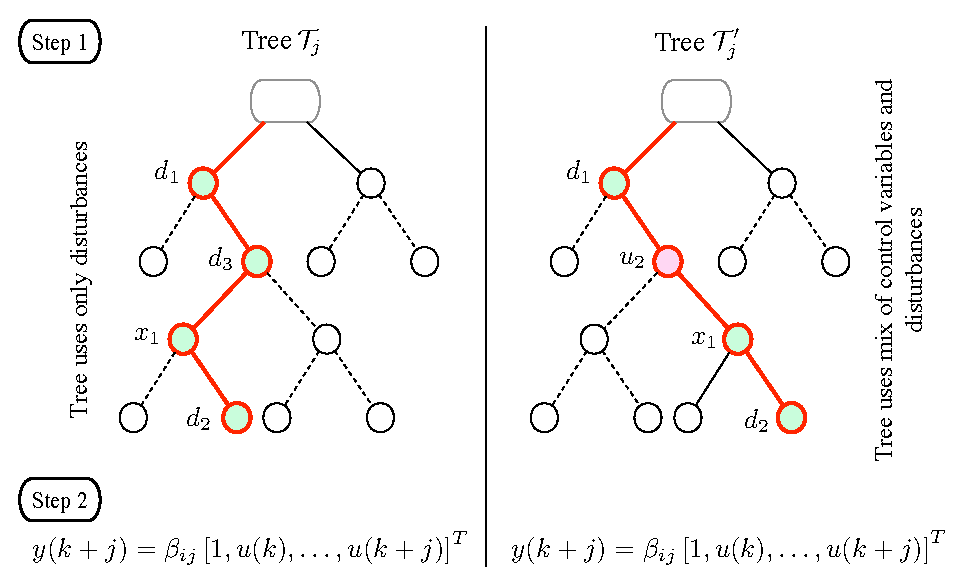
\includegraphics[width=20pc]{figures/dpc-sepvars.eps}

	\caption{\textit{Step 1:} Tree $\mathcal{T}_j$ trained only with variables in $\X^d$ using adapted RT algorithm. Tree $\mathcal{T}'_j$ trained with variables in $\X^d$ and control variables in $\X^c$ using classical RT algorithm. \textit{Step 2:} In the leaf $\ell_i$ of the tree an affine model $\beta_{ij}$ is defined as a function only of the control variables dataset corresponding to leaf $\ell_i$.}

	\captionsetup{justification=centering}

	\label{F:dpc-sepvars}

\end{figure}


\textcolor[rgb]{0,0,1}{Our modification of the Regression Tree algorithm first partitions the features set $\X$ into the sets $\X^c = \{u(k)\}_{k=1}^n\subset\X$, containing the control (or manipulated) variables, and $\X^d = \{(x(k),d(k))\}_{k=1}^n\subset\X$, containing the disturbance and state (or non-manipulated) variables. The  union of the two non-intersecting sets forms the full feature set of training $\X \equiv \X^c \cup \X^d$.
%Our goal is to replace a model-based controller with a data-driven controller, where the latter depends only on the historical sensor data. 
%These measurements could directly represent one or more states in the model-based control framework. We denote these as responses $\Y \in \R$ for training, i.e. a $\Y$ represents a particular response and we can have separate models for multiple responses. We define the number of training samples by $|(\X,\Y)| = n$.
Then the training process is divided into the following two steps, which generate as output a tree $\mathcal{T}_j$ as illustrated in Figure~\ref{F:dpc-sepvars} (left):
\begin{enumerate}
	\item the splitting of the dataset only partitions $\X^d$ (see Appendix 1 and \cite{hastie2009elements} for technical details): this choice is necessary to make our model suitable for control, as we will clarify later on, and also reduces the computational complexity. To each leaf $\ell_i$ will correspond an equivalence class of data samples $\X^d_i$ of the partition of $\X^d$, with $\X^d_i\subset \X^d$: as a consequence at any time $k$, given $\delta_d$ autoregressive terms of the disturbances and $\delta_x$ autoregressive terms of the state, we can associate $( d(k+j-\delta_d),\ldots,d(k+j),x(k-\delta_x),\ldots,x(k) )$, to the corresponding leaf $\ell_i$
	\begin{equation}\label{E:model_tree}
		\ell_i = \mathit{f}_{\mathcal{T}_j} \left( d(k+j-\delta_d),\ldots,d(k+j),x(k-\delta_x),\ldots,x(k)  \right)
	\end{equation}
	if and only if $( d(k+j-\delta_d),\ldots,d(k+j),x(k-\delta_x),\ldots,x(k)) \in \X^d_i$.
	\item in each leaf $\ell_i$ of the tree $\mathcal{T}_j$ we derive, solving a convex program over the data samples in the partition $\X^d_i$ associated to leaf $\ell_i$, an affine function, with coefficients $\beta_{ij}$, that relates the response $y(k+j)$ to the previous control inputs in $\X^c$:
	\begin{equation}\label{E:model_leaf}
		y(k+j) =  \beta_{ij} [1,u(k),\ldots,u(k+j) ]^T
	\end{equation}
	Clearly the coefficients $\beta_{ij}$ are different for each leaf $\ell_i$ as they are derived from different sets of samples.
\end{enumerate}
Applying the above procedure for $j=0,\ldots,N$ we build $N$ regression trees $\mathcal{T}_0,\ldots,\mathcal{T}_N$: thus, we have managed to linearize the original model dynamics via black-box modeling. Our two-step training procedure, described by the pseudo code of lines 1-11 of Algorithm~\ref{A:dpcrt}, can be computed off-line: this is an important advantage because the time required to create the model does not affect the control execution in run-time.}



\textcolor[rgb]{0,0,1}{The next problem now is: \emph{how to use this modeling framework to set up an MPC problem?} We setup the MPC optimization problem in the general case of multiple responses, i.e. $y(k)\in\mathbb{R}^{n_y},\ n_y\geq 1$, as follows:}

\begin{problem}\label{P:dpcrt}
	\begin{equation}
		\begin{aligned}
		& \underset{u_{k+j},\epsilon_j}{\mathrm{minimize}} & & \sum_{j=0}^{N} y^\top_{k+j} Q y_{k+j} + u^\top_{k+j} R u_{k+j} + \lambda\epsilon_j \\
		& \mathrm{subject\ to }                 & & y_{k+j}     =   \beta_{ij} [1,u^\top_{k},\ldots,u^\top_{k+j} ]^\top                   \\
		&                                       & & u_{k+j}    \in  \mathcal{U}                                                        \\
		&                                       & & |y_{k+j}|  \leq \bar{y}_{k+j} + \epsilon_j 										   \\
		&                                       & & \epsilon_j \geq  0							                                       \\
		&                                       & & j           =    0,\ldots,N.            									       \\
		\end{aligned}
		\label{E:dpcrt}
	\end{equation}
\end{problem}

\textcolor[rgb]{0,0,1}{Here, $Q \succeq 0 \in \mathbb{R}^{n_y\times n_y}$ and $R \succeq 0 \in \mathbb{R}^{n_u\times n_u}$ are weight matrices used to tradeoff the importance we provide in the minimization of $y$ versus $u$. The slack variables $\epsilon_j$ are added to ensure recursive feasibility: we relax the equality constraint on $y$ allowing violation up to $\epsilon_j$ to guarantee that Problem \ref{P:dpcrt} can provide a solution at each step $k \geq 0$. The weight $\lambda$ is then used to tradeoff the importance we provide in the optimal solution to the constraints violation versus the quadratic term. For example in the following sections we will use $\epsilon_j$ and $\lambda$ to define our tolerance to the violation of prescribed bounds by the rooms' temperature.\\
Clearly different cost functions can be chosen depending upon the application, i.e. they can be linear, nonlinear, etc., obviously changing the complexity of the problem. In the current formulation, the data-driven control problem, is reduced to a convex program which is very easy and efficient to solve in C, C++, Python and Matlab, and thus is easily integrable in SCADA systems. Indeed Problem \ref{P:dpcrt} is solved as in the classical MPC formulation, i.e. at each time step $k=1,2,\ldots$ the optimal control sequence $u^*_k,\ldots,u^*_{k+N}$ is computed, and only the first input of the sequence is applied to the system: $u(k) = u^*_k$.\\
Note that each tree $\T_j$ contributes to Problem  \ref{P:dpcrt} with the linear constraint $y_{k+j} = \beta_{ij} [1,u^\top_{k},\ldots,u^\top_{k+j} ]^\top$ as a replacement for the state dynamics in the classical MPC formulation. As a consequence, when solving Problem \ref{P:dpcrt} at time $k$, we need to determine the affine functions $\beta_{ij}$: it follows by Equation \eqref{E:model_tree} that, to determine $\beta_{ij}$ at time $k$, the knowledge of the state and disturbance measurements $\left( d(k+j-\delta_d),\ldots,d(k+j),x(k-\delta_x),\ldots,x(k) \right)$ is needed, however, values of $d(k+j-\delta_d),\ldots,d(k+j),\ j=0,\ldots,N$ are not available at time $k$, so we need to use disturbance forecast $\tilde d(k+N),\ldots,\tilde d(k)$. Using this information we can narrow down to a leaf in each tree using \eqref{E:model_tree} and thus retrieve the affine model with $\beta_{ij}$ in \eqref{E:model_leaf} for each step $j=0,\ldots,N$ of the horizon. The run-time solution of Problem \ref{P:dpcrt} illustrated above is described by the pseudo code of lines 12-23 of Algorithm~\ref{A:dpcrt}.}

\textcolor[rgb]{0,0,1}{\begin{remark}
It is now easy to understand that using the classical Regression Tree algorithm, e.g. using also the input variable $u$ in the data splitting procedure to create the trees as in the right side of Figure~\ref{F:dpc-sepvars}, the resulting model would not be suitable for control. Indeed, since $u$ is the variable we want to optimize in Problem \ref{P:dpcrt}, at time $k$ we have still not chosen its value at times $k, \ldots, k+N$: as a consequence the affine functions \emph{parameters }$\beta_{ij}$ needed to set up Problem \ref{P:dpcrt} cannot be determined at time $k$.
\end{remark}}


\textcolor[rgb]{0,0,1}{The pseudo code for the whole DPC-RT procedure (i.e. Off-line and Run-time) is given in Algorithm~\ref{A:dpcrt}. Our procedure is also graphically described in Figure \ref{F:dpc-algo-rf} for the Random Forest case, providing a good intuition also for the Regression Tree case.}


\textcolor[rgb]{0,0,1}{\begin{algorithm}[ht!]
	\caption{Data Predictive Control with Regression Trees}
	\label{A:dpcrt}
	\begin{algorithmic}[1]
		\State \textsc{Design Time (Off-Line)}
		\Procedure{Model Training using Dataset Splitting}{}
		\State Set $\X^c$ $\gets$ manipulated features
		\State Set $\X^d$ $\gets$ non-manipulated features
		\State Build $N$ predictive trees with $(\X^d,\Y)$ using Regression Trees algorithm
		\ForAll{trees $\mathcal{T}_j$}
		\ForAll{leaves $\ell_i$ of $\mathcal{T}_j$}
		\State Compute parameters $\beta_{ij}$ in \eqref{E:model_leaf} using convex programming
		\EndFor
		\EndFor
		\EndProcedure
		\State \textsc{Run Time}
		\Procedure{Predictive Control}{}
		\While{$k< k_{\mathrm{stop}}$}
		\ForAll{trees $\mathcal{T}_j$}
		\State Determine the leaf $\ell_i$ using $\X^d$ as in \eqref{E:model_tree}
		\State Obtain the linear model at $\ell_i$ trained in \eqref{E:model_leaf}
		\EndFor
		\State Solve Problem \ref{P:dpcrt} to determine optimal
		\State control actions $u^*_k,\ldots,u^*_{k+j}$
		\State Apply the first input $u(k)=u^*_k$
		\EndWhile
		\EndProcedure
	\end{algorithmic}
\end{algorithm}}


%==============================================================================================================


\subsection{DPC-En: DPC with Ensemble Methods}

\label{SS:dpcrf}

\textcolor[rgb]{0,0,1}{Regression trees obtain good predictive accuracy in many domains. However, the models used in their leaves have some limitations regarding the kind of functions they are able to approximate. The problem with trees is their high variance and that they can overfit the data easily, and a small change in the data can result in a different series of splits and thus affect the prediction accuracy. This is the price to be paid for estimating a tree-based structure from the data.}

\textcolor[rgb]{0,0,1}{To address the above problems we use ensemble methods \cite{Friedman2001}, in particular Random Forests, to combine the predictions of several independent regression trees in order to improve generalizability and robustness over a single estimator. The essential idea is to average many noisy trees to reduce the overall variance in prediction. We inject randomness into the tree construction in two ways: first, we randomize the features used to define splitting in each tree; second, we build each tree using a bootstrapped or sub-sampled data set. As a consequence each tree in the forest is trained on different data, which introduces differences between the predictive models of the trees.}

\textcolor[rgb]{0,0,1}{More precisely, in DPC-En we replace each tree in Algorithm~\ref{A:dpcrt} by a forest $\F_j$ of $t$ trees $\T_{1j},\ldots,\T_{tj}$. Each tree $\T_{\kappa j}$ is trained on the basis of a different subset of features $\bar{\X}^d_{\kappa j} \subset \X^d$. As discussed in the previous section, at any time $k$, given $\delta_d$ autoregressive terms of the disturbances and $\delta_x$ autoregressive terms of the state $\left( d(k+j-\delta_d),\ldots,d(k+j),x(k-\delta_x),\ldots,x(k) \right)$, we can associate the corresponding leaf $\ell_i$ of $\T_{\kappa j}$
\begin{equation}\label{E:model_forest}
	\ell_i = \mathit{f}_{\mathcal{T}_{\kappa j}} \left( d(k+j-\delta_d),\ldots,d(k+j),x(k-\delta_x),\ldots,x(k)  \right).
\end{equation}
Also, in each leaf $\ell_i$ of tree $\mathcal{T}_{\kappa j}$ we derive an affine function $\Theta_{i \kappa j}$, that relates the response $y(k+j)$ to the previous control inputs in $\X^c$:
\begin{equation}\label{E:model_leaf_forest}
	y(k+j) =  \Theta_{i \kappa j} [1,u(k),\ldots,u(k+j) ]^T.
\end{equation}
}

%In particular, as mentioned above, each tree $\T_i$ of each forest $\F_j$ is trained using $(\bar \X^d_i,\bar\Y_i)$.

%Here $(\bar\X^c_i,\bar\Y_i)$ correspond to the in-bag samples for the trees.


\textcolor[rgb]{0,0,1}{We can now set up the MPC problem for DPC-En as follows:}
\begin{problem}\label{P:dpcrf}
	\begin{equation}
		\begin{aligned}
		& \underset{u_{k+j},\epsilon_j}{\mathrm{minimize}} & & \sum_{j=0}^{N} y^\top_{k+j} Q y_{k+j} + u^\top_{k+j} R u_{k+j} + \lambda\epsilon_j \\
		& \mathrm{subject\ to }                 & & y_{k+j}      =  \hat{\Theta}_{j} [1,u_{k},\ldots,u_{k+j} ]^\top                      \\
		&                                       & & u_{k+j}    \in  \mathcal{U}                                                        \\
		&                                       & & |y_{k+j}|  \leq \bar{y}_{k+j} + \epsilon_j 										 \\
		&                                       & & \epsilon_j \geq  0							                                     \\
		&                                       & & j           =    0,\ldots,N.            									         \\
		\end{aligned}
		\label{E:dpcrf}
	\end{equation}
\end{problem}
\textcolor[rgb]{0,0,1}{Note that, as in the DPC-RT, the crucial problem when solving Problem \ref{P:dpcrf} is determining all parameters $\hat{\Theta}_{j}$ at time $k$. We first proceed similarly to DPC-RT by using forecast of disturbances and the state measurements to determine for each tree $\T_{\kappa j}$ the corresponding leaf $\ell_i$ and thus the affine model $\Theta_{i \kappa j}$, with $\kappa = 1,\ldots,t$ and $j = 0,\ldots,N$. In DPC-En, however, we have $t$ affine models for each prediction step $j$, thus we define $\hat{\Theta}_{j} = \frac{1}{t}\sum\limits_{\kappa = 1}^{t} \Theta_{i \kappa j}$ averaging the affine models associated to all trees of forest $\F_j$. Once we are able to determine at each time $k$ the parameters $\hat{\Theta}_{j}$ of the constraints of Problem \ref{P:dpcrf}, the optimal input $u^*_k$ can be computed as described in the previous section. The overall procedure is sketched in Figure \ref{F:dpc-algo-rf}.}

\begin{figure}[t!]
	\centering
	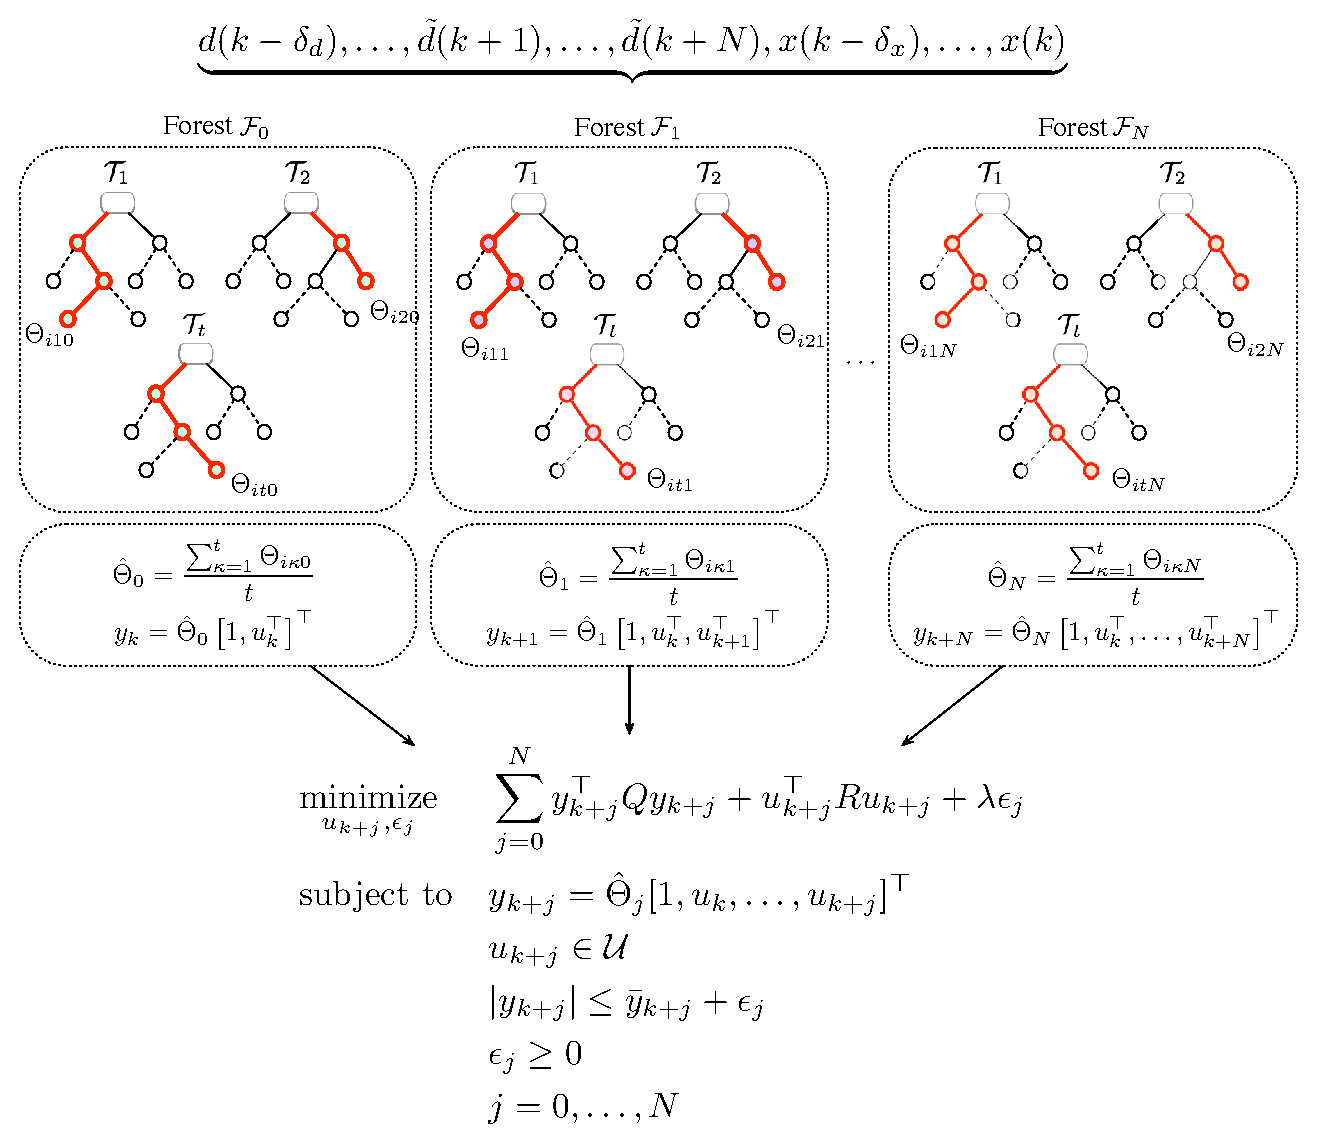
\includegraphics[width=26pc]{figures/dpc-algo-rf.eps}
	\caption{\textcolor[rgb]{0,0,1}{Graphical description of the procedure for solving Problem \ref{P:dpcrf} at each time $k$}}
	\label{F:dpc-algo-rf}
\end{figure}

\textcolor[rgb]{0,0,1}{The ensemble data predictive control (DPC-En) is the first such method to bridge the gap between ensemble predictive models (such as random forests) and receding horizon control. Reasoning on complexity, we remark that the off-line training computation in DPC-En is increased compared to DPC-RT as we need to train $t$ trees for each of the $N$ prediction steps. The run-time computation is also slightly increased as we need to derive the average $\hat{\Theta}_{j} = \frac{1}{t}\sum\limits_{\kappa = 1}^{t} \Theta_{i \kappa j}$ for each of the $N$ prediction steps. However, as shown in the following sections, it's worth the price as we obtain much better accuracy and lower variance properties with a marginal increase of the run-time computation time (the increase of off-line computation time is not a big issue as it must be run very seldom, i.e. only when a new model of the building needs to be created).}








\section{COMPARISON WITH MPC}
\label{S:proof}

We consider a bilinear building model developed at Automatic Control Laboratory, ETH Zurich.
It captures the essential dynamics governing the zone-level operation while considering the external and the internal thermal disturbances. 
By Swiss standards, the model used for this study is of a heavyweight construction with a high window area fraction on one facade and high internal gains due to occupancy and equipments \cite{Gyalistras2010a}. 

The bilinear model is a standard building model used for practical considerations \cite{Ma2015,Oldewurtel2011,Oldewurtel2012} as it is detailed enough and suitable for model-based control unlike the ones obtained from simulation software like EnergyPlus. We specifically consider this model to show a comparison against MPC. 
MPC of EnergyPlus models can be cost and time prohibitive, making them unsuitable for control. In Sec.~\ref{S:casestudy}, we show how DPC scales easily to such large scale models.

\subsection{Bilinear Model}
\label{SS:model}
%The building is treated as a lumped-parameter system, which assumes nodes in the room as well as in the walls, floor, and ceiling describing the respective temperatures.
%Considering the heat transfer rate between the nodes, an equivalent thermal RC network is identified. 
%The influence of the actuators is modeled according to their heat transfer properties, e.g. the heating input from the radiator goes directly into the room node, whereas floor heating affects the room with some delay and therefore the control input from floor heating goes into the node in the floor.

The bilinear model has 12 internal states including the inside zone temperature $\mathsf{T}_{\mathrm{in}}$, the slab temperatures $\mathsf{T}_{\mathrm{sb}}$, the inner wall $\mathsf{T}_{\mathrm{iw}}$ and the outside wall temperature $\mathsf{T}_{\mathrm{ow}}$. The state vector is defined as $x:=[\mathsf{T}_{\mathrm{in}}, \mathsf{T}_{\mathrm{sb}}^{(1:5)}, \mathsf{T}_{\mathrm{ef}}^{(1:3)}, \mathsf{T}_{\mathrm{in}}^{(1:3)}]^T$.

There are 4 control inputs including the blind position $\mathsf{B}$, the gains due to electric lighting $\mathsf{L}$, the evaporative cooling usage factor $\mathsf{C}$, and the heat from the radiator $\mathsf{H}$ such that $u:=[\mathsf{B},\mathsf{L},\mathsf{H},\mathsf{C}]^T$. $\mathsf{B}$ and $\mathsf{L}$ affect both room illuminance and temperature due to heat transfer whereas $\mathsf{C}$ and $\mathsf{H}$ affect only temperature.

The model is subject to 5 weather disturbances: solar gains with fully closed blinds $\mathsf{Q}_{\mathrm{sc}}$ and with open blinds $\mathsf{Q}_{\mathrm{so}}$, daylight illuminance with open blinds $\mathsf{I}_{\mathrm{o}}$, external dry-bulb temperature $\mathsf{T}_{\mathrm{db}}$ and external wet-bulb temperature $\mathsf{T}_{\mathrm{wb}}$. 
The hourly weather forecast, provided by MeteoSwiss, was updated every 12 hrs. Therefore, to improve the forecast,  an autoregressive model of the uncertainty was considered.
Other disturbances come from the internal gains due to occupancy $\mathsf{Q}_{\mathrm{io}}$ and due to equipments $\mathsf{Q}_{\mathrm{ie}}$ which were assumed as per the Swiss standards \cite{Merkblatt2006}. We define $d:=[\mathsf{Q}_{\mathrm{sc}},\mathsf{Q}_{\mathrm{so}},\mathsf{I}_{\mathrm{o}},\mathsf{Q}_{\mathrm{io}},\mathsf{Q}_{\mathrm{ie}},\mathsf{T}_{\mathrm{db}},\mathsf{T}_{\mathrm{wb}}]^T$. For further details, we refer the reader to \cite{Oldewurtel2011}.

The model dynamics are given below. The bilinearity is present in both input-state, and input-disturbance.
\begin{gather}
\label{E:bilinear1}
x_{k+1} = Ax_{k}+(B_u +B_{xu}[x_k] + B_{du}[d_k]) u_k+B_dd_k \\
x_{k} \in \mathbb{R}^{12}, u_{k} \in \mathbb{R}^{4}, d_{k} \in \mathbb{R}^{8} \ \forall k = 0,\dots,T, \nonumber
\end{gather}
where, the matrices $B_{xu}$ and $B_{du}$ are defined as
\begin{gather}
\label{E:bilinear2}
B_{xu}[x_k] = [ B_{xu,1}[x_k],B_{xu,2}[x_k], \dots, B_{xu,4}[x_k] ] \in \mathbb{R}^{12\times4}, \nonumber\\
B_{du}[d_k] = [ B_{du,1}[d_k],B_{du,2}[d_k], \dots, B_{du,4}[d_k] ] \in \mathbb{R}^{12\times4}\nonumber, \\
B_{xu,i} \in \R^{12\times12}, B_{du,i} \in \R^{12\times8} \ \forall i=1,2,3,4.\nonumber
\end{gather}
For this study, we assume that the disturbances are precisely known to MPC as well as DPC controller. In our future work, we will account for the uncertainties in the disturbances with an extension to Scenario approach \cite{Bernardini2009} for DPC.

\subsection{Model Predictive Control}
\label{SS:mpc}
We use an MPC controller with a quadratic and a linear cost for comparison.
The finite RHC approach involves optimizing a cost function subject to the dynamics of the system and the constraints, over a finite horizon of time \cite{Mayne2000}. After an optimal sequence of control inputs are computed, the first input is applied, then at the next step the optimization is solved again.

%\begin{figure}
%\centering
%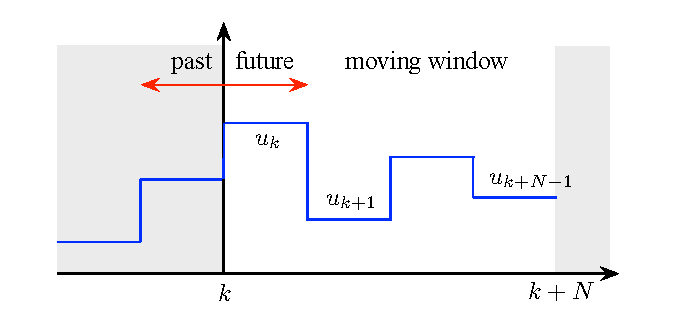
\includegraphics[scale=0.8]{figures/mpc_horizon.eps}
%\caption{Finite-horizon moving window of MPC: at time $k$, the MPC optimization problem is solved for a finite length window of $N$ steps and the first control input $u_k$ is applied; the window then recedes one step forward and the process is repeated at time $k+1$.}
%\captionsetup{justification=centering}
%\label{F:mpc}
%\end{figure}

The objective of the controller is to minimize the energy usage $c^Tu$ while maintaining a desired level of thermal comfort $x_{ref}$.
Therefore, at time step $k$, we solve a continuously linearized MPC problem to determine the optimal sequence of inputs $[u_{\mathrm{k|k}},\dots,u_{\mathrm{k+N-1|k}}]$:
\begin{subequations}
\begin{align}
\text{min } & \sum_{j=1}^{N} ({x}^T_{\mathrm{k+j|k}} - x_{ref}) \mathcal{Q} ({x}_{\mathrm{k+j|k}} - x_{ref}) + c^Tu_{\mathrm{k+j-1}} +  \lambda\epsilon_j\\
\text{s.~t. } & \ \ x_{\mathrm{k+j|k}} =  Ax_{\mathrm{k|k}} + B u_{\mathrm{k+j-1|k}} + B_d d_{\mathrm{k+j-1|k}} \label{SE:mpc1} \\
& \ \ \ \ \ B = B_u + B_{xu}[x_{\mathrm{k|k}}] + B_{du}[d_{\mathrm{k+j-1|k}}] \label{SE:mpc2}\\
& \ \ \ \ \ \ \ \ \ \ \ \ \ \ \ \underline{u} \leq u_{\mathrm{k+j-1|k}} \leq \bar{u}\\ 
& \ \ \ \ \ \ \ \ \ \ \ \ \underline{x}-\epsilon_j \leq x_{\mathrm{k+j|k}} \leq \bar{x} + \epsilon_j\\\
& \ \ \ \ \ \ \ \ \ \ \ \ \ \ \epsilon_j \geq 0, \ j = 1,\dots,N,
\end{align}\label{E:mpc}
\end{subequations} 
\noindent where $\mathcal{Q} \in \R^{12 \times 12}$ has all zeros except at $\mathcal{Q}^{(1,1)}$ corresponding to the zone temperature, $c \in \R^{4}$ is proportional to cost of using each actuator and $\lambda$ penalizes the slack variables.

\subsection{Data Predictive Control}
\label{SS:dpc}
In this section, we explain how DPC can be applied to this case study. We begin with a description of features $\tX$ and output $\tY$ used for training.

\subsubsection{Training Data} 
\label{SSS:dpc_data}

The fundamental reason why DPC  is suitable for such a problem is that when the complexity rises, there is a huge cost to model all the states given by the dynamical system \eqref{E:bilinear1}. For example, states in the bilinear model also include slab temperatures which require modeling of structural and material properties in detail and often we also need to install new sensors to capture additional states. Thus, DPC is based solely on one state of the model i.e. the zone temperature that can be easily measured with a thermostat. This serves as the output variable $\tY$ of interest for which we build $N$ trees and $N$ forests as described in Sec.~\ref{SS:dpcrt} and \ref{SS:dpcrf}, respectively. Therefore, $\tY_{\mathrm{k+j|k}}:=x_{\mathrm{k+j|k}}^1$, where $x^1$ is the first component of $x$.
Next, we define the non-manipulated features $\tX^d_{\mathrm{k|k}}$. At time $k$, for the tree $\mathcal{T}_j$ and the forest $\mathcal{R}_j$, we base these features to include weather disturbances, external disturbances due to occupancy and equipments, and autoregressive terms of the room temperature, i.e.
$\tX^d_{\mathrm{k|k}}:=[ d_{\mathrm{k+j-N|k}} ,\dots,d_{\mathrm{k+j-1|k}}, x_{\mathrm{k|k}}^1,\dots, x_{\mathrm{k-\delta|k}}^1 ]$, where $\delta$ is the order of autoregression.
Finally, the inputs in DPC are exactly same as in MPC. i.e. $\tX^c_{\mathrm{k+j-1|k}}:=u_{\mathrm{k+j-1|k}}$.

The training data in the above format was generated by simulating the bilinear model with rule-based strategies for 10 months in 2007. January and May were deliberately excluded for testing the DPC implementation.

\subsubsection{Optimization} 
\label{SSS:dpc_opt}
For a fair comparison with MPC, we cast DPC optimization problem as follows:
\begin{subequations}
\begin{align}
\text{min } & \sum_{j=1}^{N} {\tY}_{\mathrm{k+j|k}} \mathcal{Q}^{(1,1)} {\tY}_{\mathrm{k+j|k}} + c^T \tX^c_{\mathrm{k+j-1|k}}+  \lambda\epsilon_j\\
\text{s.~t. } & \ \ \ \ \ \tY_{\mathrm{k+j|k}} =  \alpha_j^T \left[1,\tX^c_{\mathrm{k|k}},\dots,\tX^c_{\mathrm{k+j-1|k}} \right]^T \label{SE:dpc}\\
& \ \ \ \ \ \ \ \ \ \ \ \ \ \ \ \underline{\tX}^c \leq \tX^c_{\mathrm{k+j-1|k}} \leq \bar{\tX}^c\\ 
& \ \ \ \ \ \ \ \ \ \ \ \ \underline{\tY}-\epsilon_j \leq \tY_{\mathrm{k+j|k}} \leq \bar{\tY} + \epsilon_j\\\
& \ \ \ \ \ \ \ \ \ \ \ \ \ \ \epsilon_j \geq 0, \ j = 1,\dots,N.
\end{align} \label{E:dpc}
\end{subequations}
\noindent Here $\alpha = \beta$ for DPC-RT and $\alpha = \hat{\Theta}$ for DPC-En.
Note that, \eqref{E:dpc} is DPC analog of \eqref{E:mpc}. The only difference is the state dynamics \eqref{SE:mpc1} and \eqref{SE:mpc2} are now replaced with \eqref{SE:dpc}.

\subsubsection{Validation} 
\label{SSS:dpc_val}

We compare the prediction for the first time step $\tY_{\mathrm{k+1|k}}$ and the 6-hour ahead prediction $\tY_{\mathrm{k+6|k}}$ for a week in the month of May in Fig.~\ref{F:validation}. It is visible how trees have a high variance, and the forests are more accurate. Note that data from January and May was not used for training. The quantitative summary of the accuracy is given in Tab.~\ref{T:validation}. We can see that the random forests are better in all respects.
\begin{table}[h!]
	\centering
	\begin{tabular}{cccc}
		\toprule
		& RMSE & $R^2$ score & EV  \\ 
		\midrule
		tree-$\tY_{\mathrm{k+1|k}}$    &  0.42 &  0.75 & 0.76    \\
		tree-$\tY_{\mathrm{k+6|k}}$  & 0.64 &  0.41  & 0.42 \\
		forest-$\tY_{\mathrm{k+1|k}}$  & 0.29 & 0.87  & 0.88 \\
		forest-$\tY_{\mathrm{k+6|k}}$  & 0.38 & 0.78 & 0.80 \\
		\bottomrule
	\end{tabular}
	\caption{Quantitative comparison of root mean square error (RMSE), $R^2$ score, and explained variance (EV) for trees and forests for different predictions steps.}
	\captionsetup{justification=centering}
	\label{T:validation}
\end{table}

\begin{figure}[h!]
	\centering
	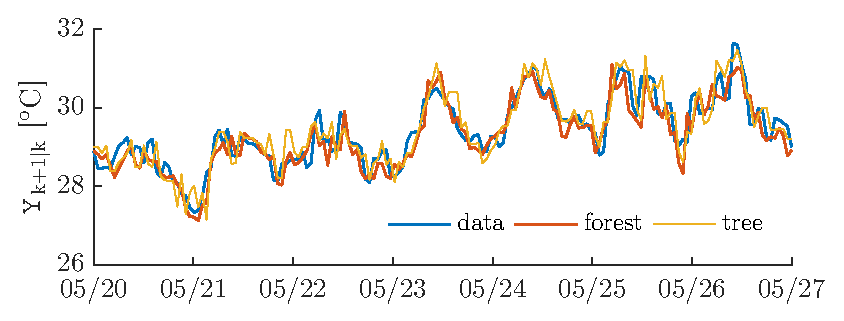
\includegraphics[width=20pc]{figures/validation-s1.eps}
	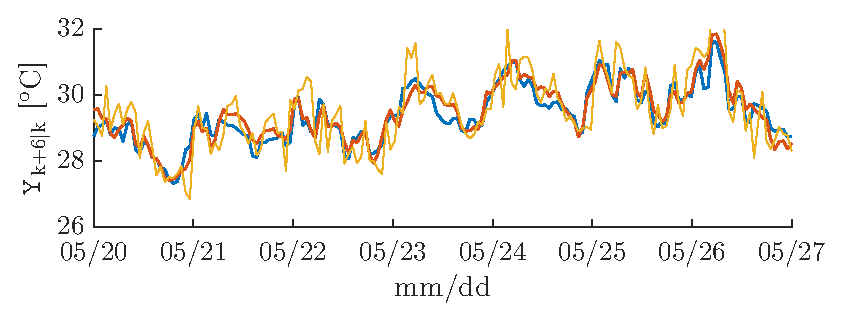
\includegraphics[width=20pc]{figures/validation-s6.eps}
	\caption{Temperature predictions from a tree and a forest for first step prediction (top) and the 6-hour ahead prediction (bottom). Ensemble method shows a relatively higher accuracy.}
	\captionsetup{justification=centering}
	\label{F:validation}
\end{figure}

%\begin{figure}[t!]
%	\centering
%	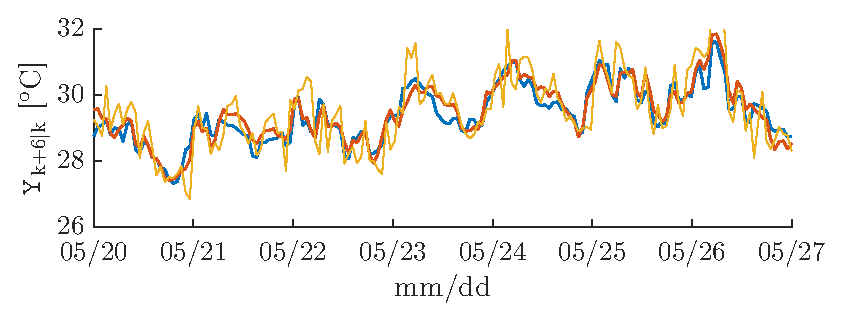
\includegraphics[width=20pc]{figures/validation-s6.eps}
%	\caption{Temperature predictions from a tree and a forest for 6 hour ahead prediction.}
%	\captionsetup{justification=centering}
%	\label{F:validation-s6}
%\end{figure}

\subsection{Comparison}
\label{SS:comp}
We compare the performance of DPC \eqref{E:dpc} against an equivalent MPC formulation \eqref{E:mpc}. The solution obtained from MPC sets the benchmark that we compare to. Note that the MPC implementation uses the exact knowledge of the plant dynamics. Therefore, the associated control strategy is indeed the optimal strategy for the plant.

The performance is compared for 3 days in winter, i.e. January 28-31 and 3 days in summer, i.e. May 1-3. These are shown on the same plots in Figure~\ref{F:comparison}.
The sampling time in the simulations is 1 hr. The control horizon $N$ and the order of autoregression are both 6 hrs. The training procedure required a few minutes in the case of trees and 2 hrs for forests on a Win 10 machine with an i7 processor and 8GB memory.
The cooling usage factor $\mathsf{C}$ is constrained in $[0,1]$, the heat input in $[0,23]\ \mathrm{W/m^2}$, and the room temperature in $[19,25]\ \mathrm{^oC}$ during the winters and $[20,26]\ \mathrm{^oC}$ during the summers.
The optimization is solved using CPLEX \cite{IBM}.

The external disturbances - solar gain, internal gain due to equipment and dry-bulb temperature during the chosen periods are shown in Figure~\ref{F:dist}. The internal gain due to occupancy was proportional to the gain due to equipment. 
The reference temperature is chosen to be 22 $\mathrm{^oC}$. Due to cold weather, which is evident from the dry-bulb temperature, the heating system is switched on during the night to maintain the thermal comfort requirements. When the building is occupied during the day, due to excessive internal gain, the building requires cooling. The lighting in the building is adjusted to meet the minimum light requirements.
The optimal cooling usage factor and the radiator power for MPC, DPC-En and DPC-RT are shown in Figure~\ref{F:control1} and Figure~\ref{F:control2}, respectively. The control strategy with DPC-En shows a remarkable similarity to MPC, switching on/off the equipments at the same time with similar usage. However, the performance with DPC-RT is much different and worse. DPC-RT inherently suffers from high variance which is also evident in the control strategy, thus making it unsuitable for practical purposes. 
Although it seems like that adding the rate constraints to DPC-En would smoothen its behavior, this was avoided because the sampling time of the system is 1 hr which is already too high. The room temperature profile in Figure~\ref{F:state} is close to the reference in the case of DPC-En as well as MPC. 
Figure~\ref{F:obj} shows that the cumulative cost of the objective function is, as expected, minimum for MPC, and a bit higher for DPC-En. The cost for DPC-RT blows up around 12 noon on 30$^{th}$ January as one of the slack variables is non-zero, which happens due to high model inaccuracy.

The quantitative performance comparison is shown in Table~\ref{T:comparison}. MPC tracks the reference more closely at the expense of higher input costs in comparison to DPC-En. The higher cost of the inputs in MPC is also due to lighting. DPC-En explains 70.1\% variation in the optimal control strategies obtained from MPC while DPC-RT explains only 1.8\%. The mean optimal cost of DPC-En is more than MPC, and is maximum for DPC-RT due to a constraint violation.

\begin{table}[h!]
	\centering
	\begin{tabular}{ccccc}
		\toprule
		& explained & mean objective& mean input  & mean  \\
		&  variance$[\mathrm{-}]$ & value $[\mathrm{-}]$ & cost $[-]$ & deviance $[\mathrm{^oC}]$ \\     
		\midrule
		MPC    &  $\mathrm{-}$ &  22.60 & 17.16  &  0.26  \\
		DPC-En   & 70.1\% &  39.26  & 15.12 &  0.48 \\
		DPC-RT  & 1.8\% & 204.55 & 16.84 &  0.57 \\
		\bottomrule
	\end{tabular}
	\vspace{0.2cm}
	\caption{Quantitative comparison of explained variance, mean value of objective function, mean input cost $c^Tu$ and mean deviance from the reference temperature $|\mathsf{T}-\mathsf{T}_{\mathrm{ref}}|$.}
	\captionsetup{justification=centering}
	\label{T:comparison}
\end{table}

\begin{figure}[t!]
	\begin{center}
	\vspace{1.1cm}
	\subfigure[External disturbances: solar gain, internal gain due to equipment and dry-bulb temperature.]{
		\label{F:dist}
		\centering
		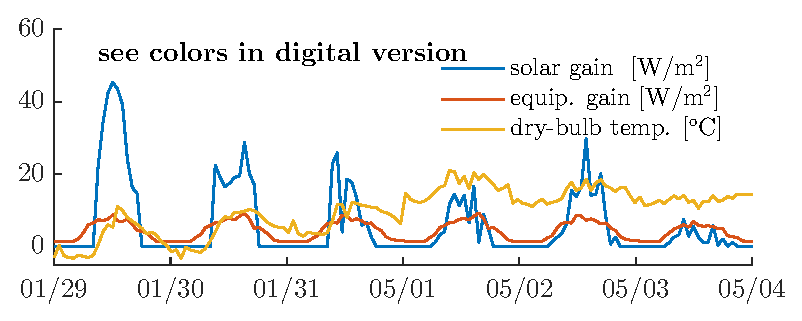
\includegraphics[width=25pc]{figures/disturbances.eps}
	}

	\subfigure[Optimal control input: cooling usage factor $\mathsf{C}$ with  $0 \leq \mathsf{C} \leq 1$. DPC-En generates a control strategy very simular to MPC.]{
		\label{F:control1}
		\centering
		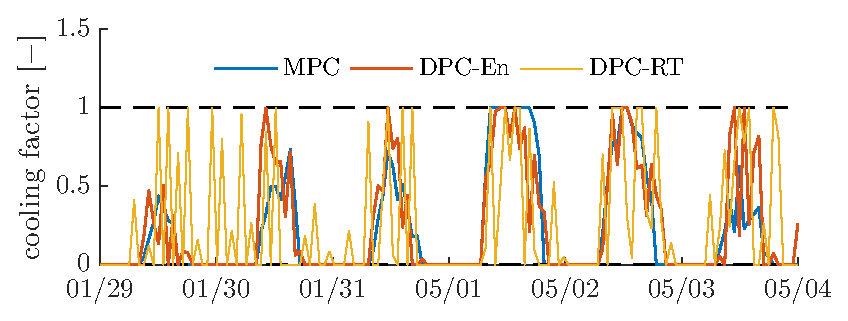
\includegraphics[width=25pc]{figures/input3.eps}
	}

\end{center}
\end{figure}
\begin{figure}[h!]
\begin{center}
	\subfigure[Optimal control input: radiator heat $\mathsf{H}$ with  $0 \leq \mathsf{H} \leq 23 \ \mathrm{W/m^2}$. Again, DPC-En generates a control strategy very simular to MPC.]{
		\label{F:control2}
		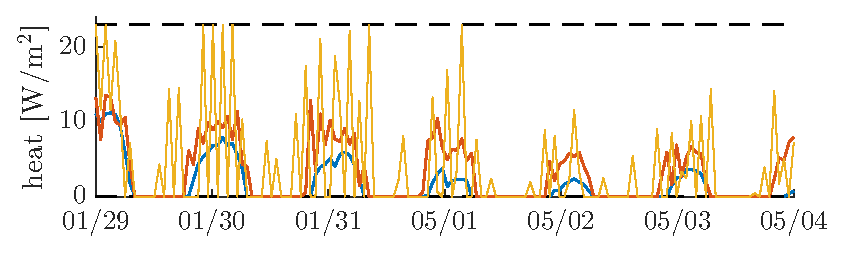
\includegraphics[width=25pc]{figures/input4.eps}
	}

	\subfigure[Room temperature has time varying bounds. When the building is occuped the constraints are relaxed, else $19(20) \leq \mathsf{T}_{\mathrm{in}} \leq 25(26) \ \mathrm{^oC}$ in January(May). MPC and DPC-En are able to track the reference temperature ($22 \ \mathrm{^oC}$) closely.]{
		\label{F:state}
		\centering
		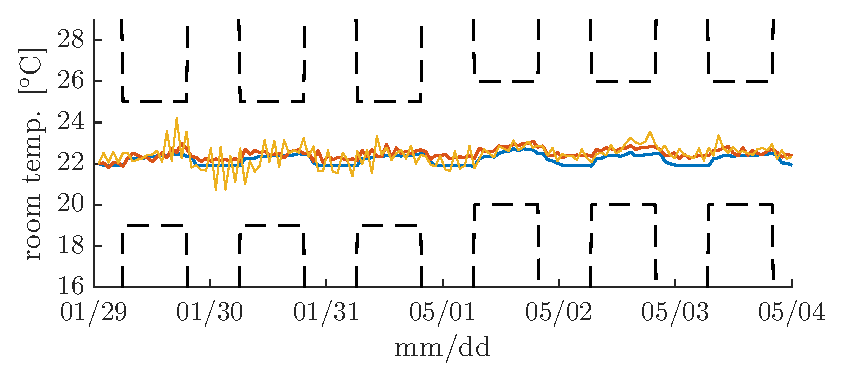
\includegraphics[width=25pc]{figures/state.eps}
	}

	\subfigure[Cumulative optimal cost after solving optimization. MPC serves as the benchmark with the minimum cost, followed by DPC-En and then DPC-RT.]{
		\label{F:obj}
		\centering
		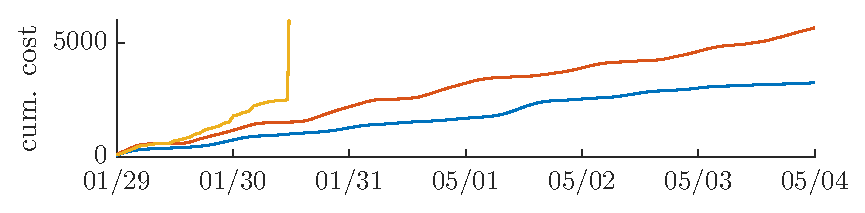
\includegraphics[width=25pc]{figures/cumsumcost.eps}
	}
	\end{center}
	%\vspace{-1cm}
	\caption{Comparison of optimal performance obtained with MPC, DPC-En and DPC-RT for 3 days in January and 3 days in May.}
	\label{F:comparison}
	\captionsetup{justification=centering}
\end{figure}
Thus, we have shown that DPC-En provides a comparable performance to MPC without using the physical model.
However, one major limitation of the bilinear model is that the information about the building power consumption is not available. Much nonlinearities in the system are due to equipment efficiencies which are not considered in the bilinear case but are very important for practical purposes. 

Therefore, our next goal is to apply DPC-En on even more complex and realistic EnergyPlus model for which building a model predictive controller is time and cost prohibitive \cite{Sturzenegger2016}. This is because we would need to model intricate details like the geometry and construction layouts, the equipment design and layout plans, material properties, equipment and operational schedules etc.




\section{APPLICATION: DEMAND RESPONSE}
\label{S:casestudy}

In January 2014, the east coast (PJM) electricity grid experienced an 86x increase in the price of electricity from \$31/MWh to \$2,680/MWh in a matter of 10 minutes. Similarly, the price spiked 32x from an average of \$25/MWh to \$800/MWh in July of 2015. This extreme price volatility has become the new norm in our electric grids. Building additional peak generation capacity is not environmentally or economically sustainable. Furthermore, the traditional view of energy efficiency does not address this need for \emph{Energy Flexibility}. The solution lies with Demand Response (DR) from the customer side - curtailing demand during peak capacity for financial incentives. However, this is a very hard problem for commercial, industrial and institutional plants, the largest electricity consumers.
%the cost to model each building is over \$100K and buildings are all unique, they cannot decide which of the 100,000's of control knobs to turn as it is too complex, they must rely on rule-based curtailment approaches which are ad hoc, inefficient and do not provide any guarantees for energy reduction and are consequently exposed to a huge financial risk.

Thus, the problem of energy management during a DR event makes an ideal case for DPC. In the following sections, we apply DPC-En to a large scale EnergyPlus model to show how effectively DPC can provide a desired power curtailment as well as a desired thermal comfort. DPC builds predictive models of a building based on historical weather, schedule, set-points and electricity consumption data, while also learning from the actions of the building operator. These models are then used for synthesizing recommendations about the control actions that the operator needs to take, during a DR event, to obtain a given load curtailment while providing guarantees on occupant comfort and operations.

\subsection{EnergyPlus Model}
We use the DoE Commercial Reference Building (DoE CRB) simulated in EnergyPlus \cite{Deru2011} as the virtual test-bed building.
This is a large 6 story hotel building consisting of 22 zones with a total area of 122,120 sq.ft. 
During peak load conditions the building can consume up to 400 kW of power. 
For the simulation of the DoE CRB building we use actual meteorological year data from Chicago for the years 2012 and 2013. 

\subsection{Model training for DPC}

In the following simulations, we consider a long DR event from 7am - 2pm when the end-users are expected to follow/track the reference power signal sent by the utility. This is indeed common in Demand Tracking Control. 
During offline training, we sample data every 15 min to learn 2 kinds of forests. (1) Power forests are built using output as the total building power consumption, and (2) Temperature forests with output as temperature of one of the 22 zones. 
The training data set contains the following types of features. (1) The \textit{weather data} which includes measurements of the outside air temperature and relative humidity. Since we are interested in predicting the power consumption or the zone temperature for a finite horizon, we include the weather forecast of the complete horizon in the training features. (2) The \textit{schedule data} includes the proxy variables which correlate with repeated patterns of electricity consumption e.g., due to occupancy or equipment schedules. Day of Week is a categorical predictor which takes values from 1-7 depending on the day of the week. This variable can capture any power consumption patterns which occur on specific days of the week. Likewise, Time of Day is quite an important predictor of power consumption as it can adequately capture daily patterns of occupancy, lighting and appliance use without directly measuring any one of them. Besides using proxy schedule predictors, actual building equipment schedules can also be used as training data for building the trees. (3) The \textit{building data} include (i) cooling set points for  the guest rooms, kitchen and corridors, (ii) supply air temperature, and (iii) chilled water temperature.
For the following simulations, we use five control variables (i) cooling set point for corridors $\mathsf{ClgSP}$, (ii) cooling set point for guest rooms $\mathsf{GuestSP}$, (iii) cooling set point for kitchen $\mathsf{KitchenSP}$, (iv) chilled water supply temperature $\mathsf{ChwSP}$, and (v) supply air temperature  $\mathsf{SupplyAirSP}$, so $u := [\mathsf{ClgSP},\mathsf{GuestClgSP},\mathsf{KitchenClgSP},\mathsf{SupplyAirSP}, \mathsf{ChwSP}]^\top$. 
The power forest $\mathcal{F}_p$ is built using the total building power consumption $\tP$. Its features in $\X^d$ include the weather variables, their lag terms and their forecast over the horizon, the schedule variables, and finally the lag terms of the power consumption.
The temperature forest $\mathcal{R}_t$ is built with zone temperature $\tT$ as the output. Except for the autoregressive terms corresponding to the same zone temperature, all other features are same in $\X^d$.
Figure~\ref{F:sepvars} shows the prediction accuracy for the power forest, and also explains the two level training approach introduced in Section~\ref{SS:sepvar}. During S1, the forests are trained using only disturbances as the features. Then in S2, the local effects of the control variables are accounted for by the linear models in the leaves. We observe how the accuracy is drastically improved after including the linear models in the predictions.

\subsection{Power Management}
\label{SS:powermanagement}
Typically, the end customer receives a notification to curtail the power by some fraction. 
In this example on power management, we show how DPC can generate optimal inputs to track a desired power signal within a small allowance while maintaining the zone level thermal comfort. It may not be possible to have the same thermal comfort level in all the zones due to power curtailment, so we choose one zone (for example CEO's office) where the constraints must be met.
\begin{figure}[t!]
	\centering
	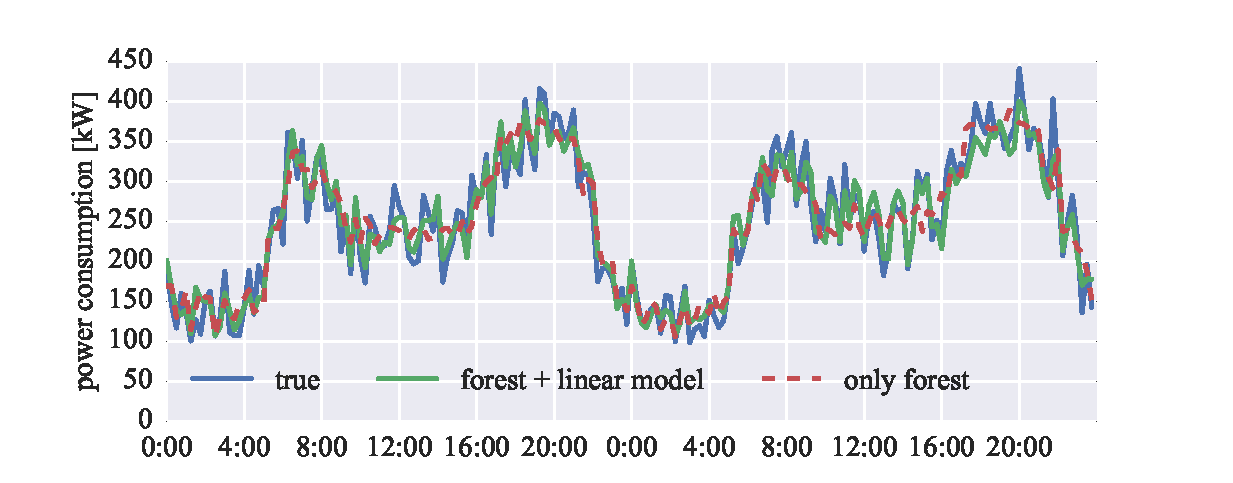
\includegraphics[width=30pc]{figures/eplus_validation.eps}	
	\caption{Model accuracy during training: The prediction made by forest using only $\X^d$ (red) captures the effect due to disturbances. The linear models in the leaves capture the local effects (green) due to the control inputs in $\X^c$ and improve the model accuracy.}
	\label{F:sepvars}
	\captionsetup{justification=centering}
\end{figure}
This is done by solving the following optimization problem, with control variables defined before:
\begin{align}
\begin{aligned}
& \underset{u_{k+j-1},\epsilon_j,\delta_j}{\mathrm{minimize}} & & \sum_{j=1}^{N} ({\tP}_{k+j} - \tP_{ref})^2 +  \lambda\epsilon_j + \nu \delta_j \\
& \mathrm{subject\ to }                                       & & \tP_{k+j} =  \hat{\Theta}_{\tP_j} [ 1,u^\top_{k},\ldots,u^\top_{k+j-1} ]^\top  \\
&                                                             & & \tT_{k+j} =  \hat{\Theta}_{\tT_j} [ 1,u^\top_{k},\ldots,u^\top_{k+j-1} ]^\top  \\
&                                                             & & \underline{\tP} - \epsilon_j \leq \tP_{k+j} \leq \bar{\tP} + \epsilon_j        \\
&                                                             & & \underline{\tT} - \delta_j   \leq \tT_{k+j} \leq \bar{\tT} + \delta_j          \\
&                                                             & & \underline{u}                \leq u_{k+j-1} \leq \bar{u}                       \\
&                                                             & & \epsilon_j \geq 0,\delta_j \geq 0, \ j = 1,\dots,N.
\end{aligned}\label{E:ptrack}
\end{align}

\begin{figure}[h!]
	\begin{center}
	\subfigure[Optimal inputs calculated by DPC-En. At first, the inputs are changed rapidly because of a significant difference between the desired and the actual power consumption. Then gradual adjustments are made to follow the desired reference.]{
		\label{F:eplus_inputs}
		\centering
		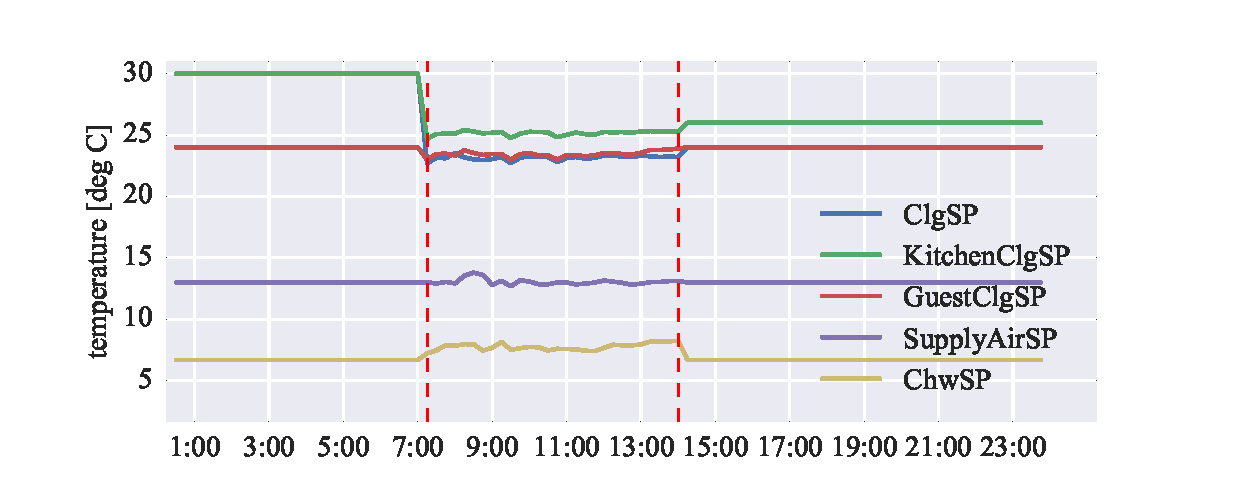
\includegraphics[width=29pc]{figures/eplus_control.eps}
	}
	\subfigure[Power tracking by DPC-En at 1.1 MW: The difference in closed-loop simulation and prediction is due to model mismatch.]{
		\label{F:eplus_power}
		\centering
		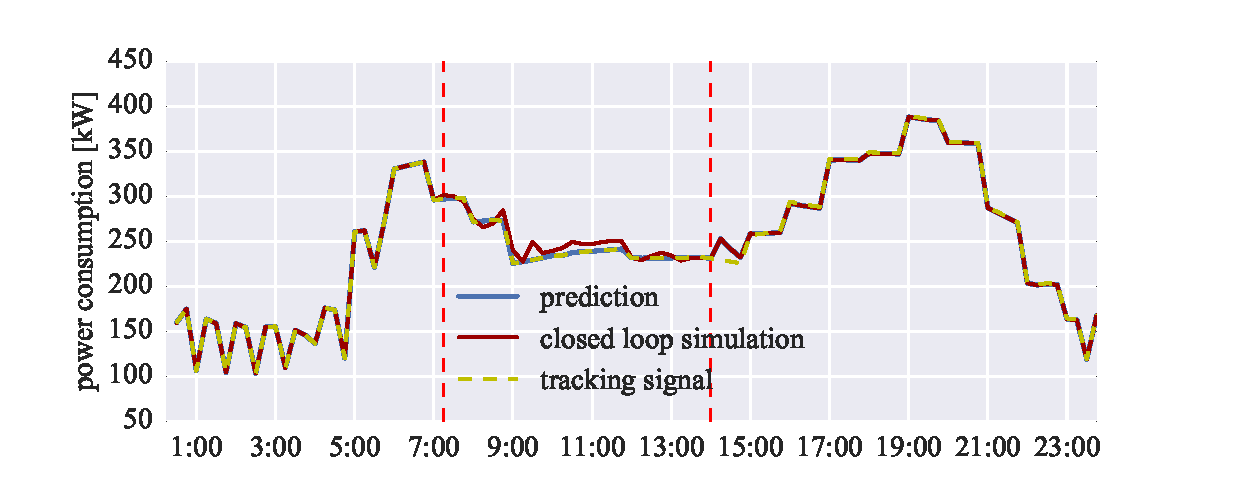
\includegraphics[width=29pc]{figures/eplus_closedloop.eps}
	}
\end{center}
	\caption{Power management using DPC. The controller is active between 7am - 2pm. This region is marked in dashed red lines.}
	\captionsetup{justification=centering}
	\label{F:eplus_track}
\end{figure}

Here, the temperature forests are used to enforce thermal constraints in the zone of interest. The setup of optimization problem is flexible to include even other variables in the cost or the constraints. For example, we are currently looking at including the dynamic pricing of electricity in the cost since the customers can more directly relate to the financial incentives.

The results are shown in Figure~\ref{F:eplus_track}. 
The DPC controller is active between 7am - 2pm. Before 7am and after 2pm, the building is using a predefined rule-based control strategy.
The optimal control inputs from DPC-En are shown in Figure~\ref{F:eplus_inputs}. It is observed that, with the optimal inputs generated by DPC, we can track the reference power consumption signal closely. In fact, the average tracking error between 7am - 2pm is 3\%. The difference between the predicted power consumption and that in the closed-loop simulation in Figure~\ref{F:eplus_power} is due to model mismatch between the EnergyPlus model and the power forest used in the optimization \eqref{E:ptrack}. Due to this inaccuracy, the actual power consumption is on an average 7 kW higher.

Thus, DPC-En successfully tracks a given power reference signal with an average $\sim$ 3\% error for such a complex building which would require several years of efforts to develop a physics based model.


\clearpage
\section{CASE STUDY: OPTIMAL HEATING SYSTEM SCHEDULING}
\label{S:realCaseStudy}

In this section, we show an application of DPC to a real house located in L'Aquila, Italy. Random forest models for DPC built using historical data from this house are described in Section \ref{SS:randomForestsModels}. 
In Section \ref{SS:energyPlusmodel}, we present the thermal energy model of the building in EnergyPlus, built using historical data, construction layout and materials after spending $\sim3$ months of efforts.
In Section \ref{SS:controllersDPCandBangbang}, we set up the DPC optimization problem and describe the bang-bang control strategy. Finally, in Section \ref{SS:simulationResults}, the performance of the two controllers are compared in terms of energy saving using the EnergyPlus model. In particular, we show that DPC allows an energy saving up to $49.2\%$ with respect to the bang-bang controller while guaranteeing thermal comfort for occupants. The section organization is graphically shown in Figure \ref{F:overview}.
\begin{figure}[h!]
	\begin{center}
		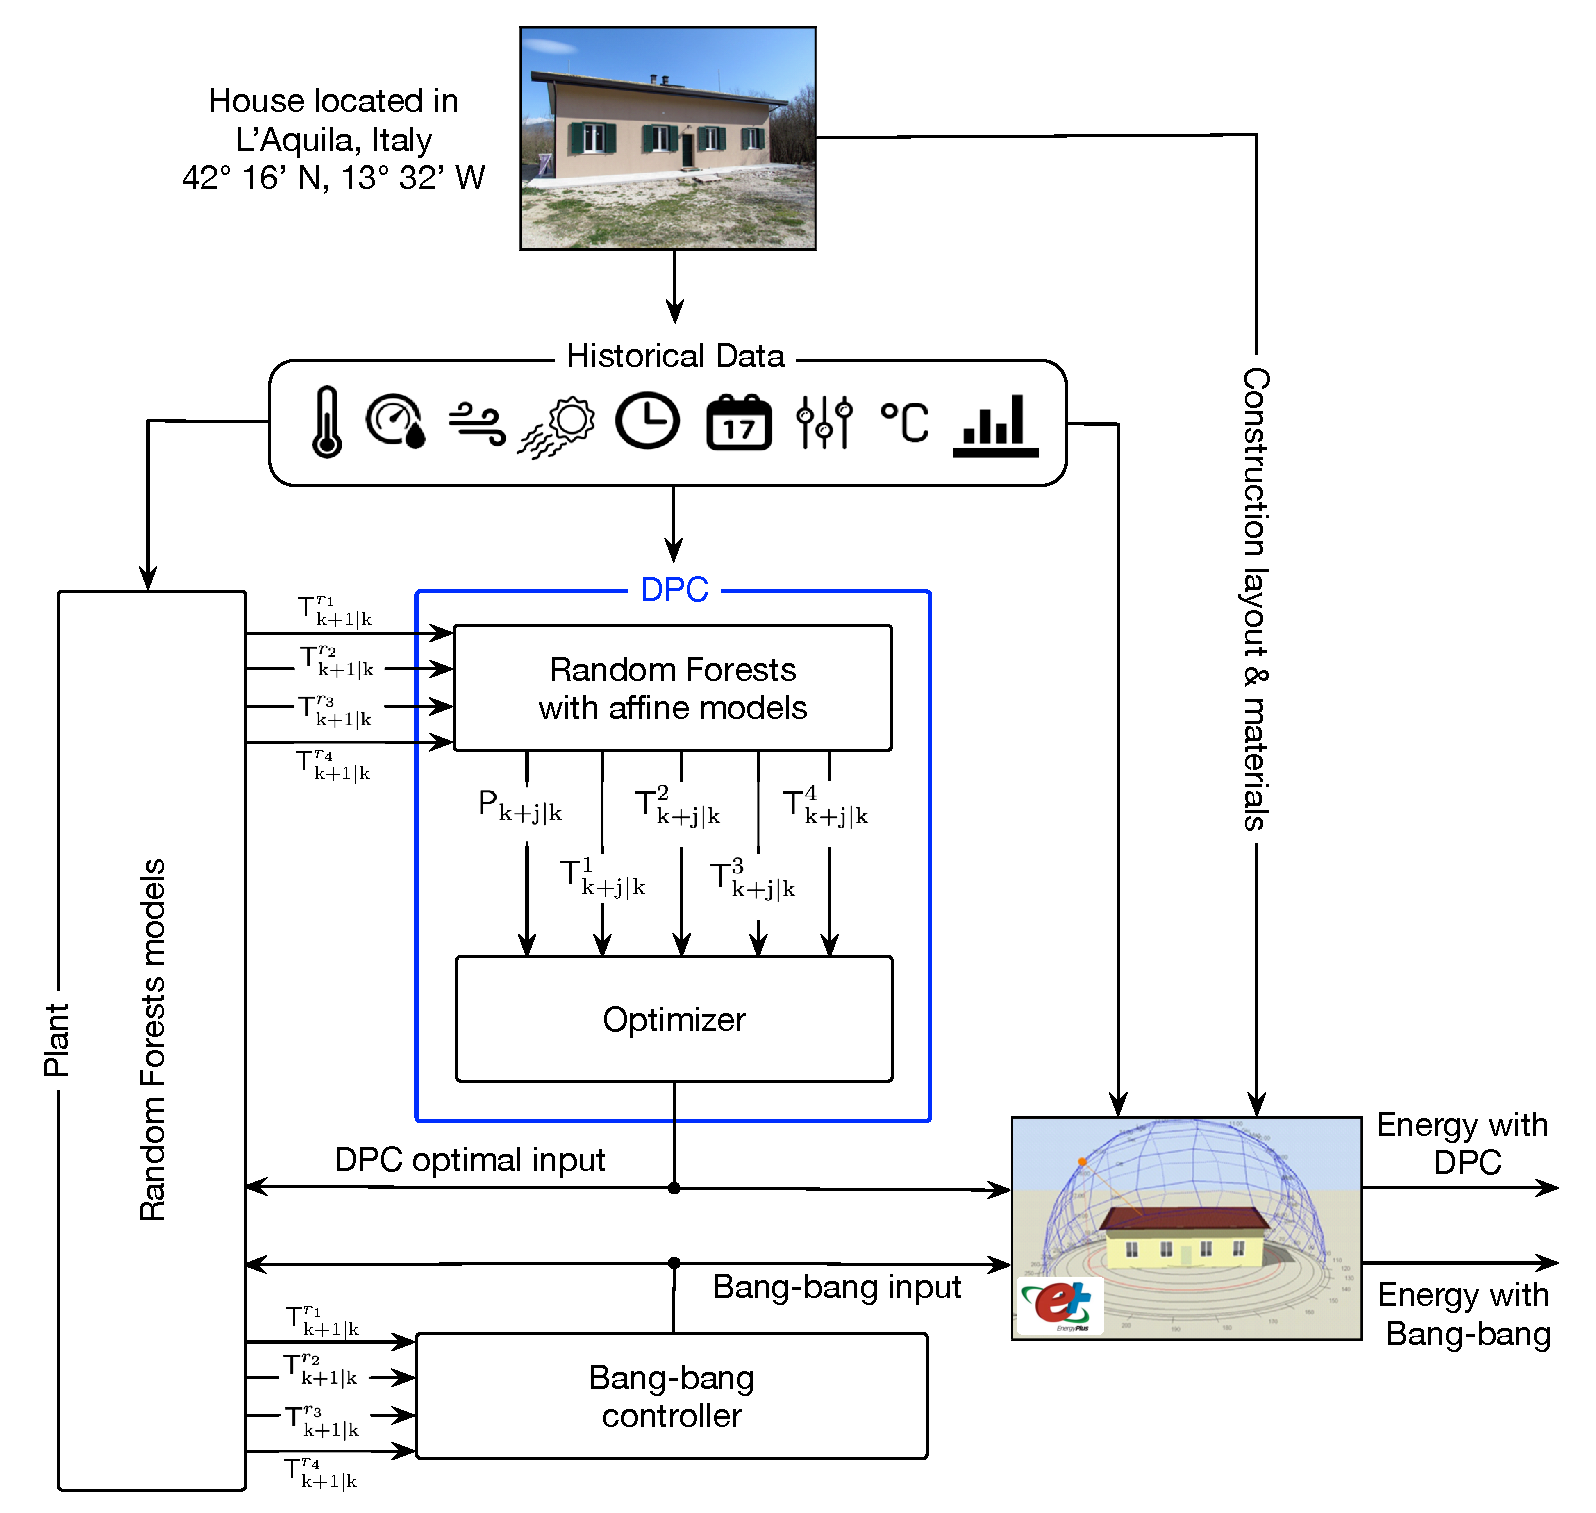
\includegraphics[width=1\linewidth]{figures/overview.eps}
		\caption{Random Forest trained on all features including the control variable are used as the plant in the closed-loop simulations with DPC and bang-bang controller. DPC optimzation uses Random Forests with affine functions as predictive models. Controllers' strategies are evaluated using the EnergyPlus model to compare the actual energy consumption.}
		\captionsetup{justification=centering}
		\label{F:overview}
	\end{center}
\end{figure}

\subsection{Description of the house}\label{SS:descriptionHouse}
The chosen case study is a detached off-grid two-story residential house, located in the outskirt of L'Aquila (coordinates $42\degree$ $16'$ latitude and $13\degree$ $32'$ longitude), Italy and is shown in Figure \ref{F:house}. The building, inhabited by the two owners, has a main north-south orientation and it is composed by a heated ground floor and an attic without heating system. Therefore, although the gross area of the house is equal to $209.5\,m^2$, the heated gross area is equal to $112.4\,m^2$.
Thanks to the off-grid characteristic, the technological plants guarantee the complete energy self-sufficiency of the building. The house is equipped with a biomass boiler, a solar thermal plant, a stand-alone photovoltaic system, black water and rainwater reuse systems and a well for water supply, and has complete independence from the utilities.   
The bearing structure of the house is made of reinforced concrete and EPS (expanded polystyrene) insulation, while the building envelope is composed by prefabricated wood-cement blocks, shown in Figure \ref{F:houseSection}, with EPS and graphite insulation, that allow low thermal fluxes. The thermal performance of a wood-cement block, with similar geometry, was investigated in a previous work \cite{Nardi2016}, both with experimental and numerical approach.
The heating system of the building, that supplies the thermal energy required in winter season, is a hydronic system consisting of a vegetable biomass boiler, with a manual ON/OFF, a constant-flow pump station, and tubular steel radiators as shown in Figure \ref{F:housePlantScheme}. The standard biomass boiler has an efficiency of $83.5\%$ with $16.5\ kW$ of thermal power transferred to the water, without gas-flame modulation. The heat transfer fluid distribution is realized through a manifold circuit, that supplies the radiators placed in the various rooms of the house. The energy needs for the domestic hot water (DHW) are covered by the same boiler, coupled with a solar thermal plant. It is worth noting that, in this work, the thermal energy needed for the domestic hot water production is neglected. 
\begin{figure}[t!]
	\begin{center}
		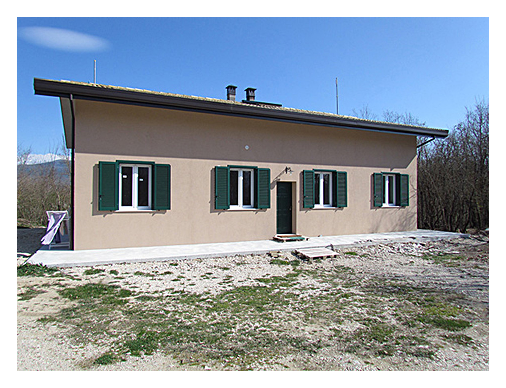
\includegraphics[width=20pc]{figures/Vista_sud.eps}
		\caption{Off-grid residential house.}
		\captionsetup{justification=centering}
		\label{F:house}
	\end{center}
%	\vspace{-0.5cm}
\end{figure}
\begin{figure}[h!]
	\begin{center}
		\subfigure[Walls.]{
			\label{F:houseSection1}
			\centering
			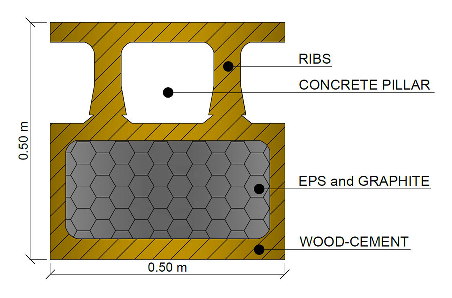
\includegraphics[width=16pc]{figures/blocco_parete_rev01.eps}
		}
		\subfigure[Floor and roof.]{
			\label{F:houseSection2}
			\centering
			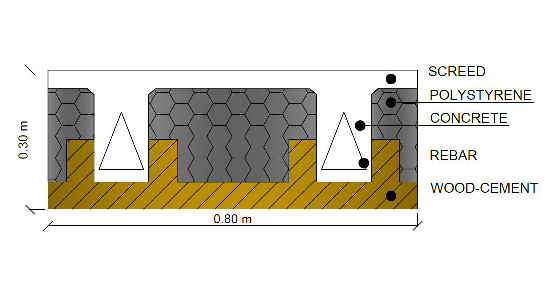
\includegraphics[width=17pc]{figures/blocco_solaio_rev01.eps}
		}
	\end{center}
	\vspace{-0.5cm}
	\caption{Cross-sections of the wood-cement blocks.}
	\captionsetup{justification=centering}
	\label{F:houseSection}
\end{figure}
For a thorough knowledge of the building thermal behavior, an in-situ analysis was carried out. Temperature measuring devices, completely self-produced at the “G. Parolini Lab” of the University of L'Aquila \cite{Pantoli2017}, mainly based on an $ATmega 2560$ microcontroller and $DS18B20$ temperature probes (temperature range from $-55.0\degree C$ to $125.0\degree C$ with an accuracy of $\pm 0.5\degree C$), were employed to acquire the ambient temperatures of $4$ differently oriented rooms of the house as shown in Figure \ref{F:houseFloors} (displayed with red dots $A1$, $A2$, $A3$ and $A4$). The probes positions were chosen to optimize the data acquisition and to minimize the discomfort of the occupants in the house. Furthermore, as can be seen in Figures \ref{F:housePlantScheme} and \ref{F:houseFloors}, a commercial heat meter (temperature range from $10.0\degree C$ to $90.0\degree C$ with an accuracy of $\pm 0.05\degree C$, displayed with orange dot $G1$) was installed downstream of the biomass boiler to measure the produced thermal energy. The turbine flowmeter was installed on the return pipe, while the two thermocouples were placed inside the delivery and return pipes, respectively. All the measuring devices have been set with a data acquisition rate equal to $10$ minutes, from March $11^{th}$ $2016$ to May $15^{th}$ $2016$.

The collected data are used in the following to create both an EnergyPlus and a random forest model for the energy consumption assessment of the house. These models will be used for performance comparison of DPC with respect to a classical bang-bang controller. In particular DPC will be set up to provide an optimal ON/OFF scheduling policy for the heating system in order to save energy while guaranteeing thermal comfort for the occupants. To this aim, we also create random forest models for power consumption and room temperatures to be used in the closed-loop simulations. 

\begin{figure}[t!]
	\begin{center}
		\includegraphics[width=27pc]{figures/Schema_di_impianto.eps}
		\caption{Technological plant scheme of the use case.}
		\captionsetup{justification=centering}
		\label{F:housePlantScheme}
	\end{center}
\end{figure}
\begin{figure}[t!]
	\begin{center}
		\subfigure[Ground floor.]{
			\label{F:houseGroundFloor}
			\centering
			\includegraphics[width=26pc]{figures/Arch_PT_e_sonde.eps}
		}
		\subfigure[Attic.]{
			\label{F:houseAttic}
			\centering
			\hspace{-1.6cm}
			\includegraphics[width=22.8pc]{figures/Arch_P1.eps}
		}
	\end{center}
	\caption{Layout of the house and probes placement. Legend: red circle for ambient temperature; orange circle for heat meter.}
	\captionsetup{justification=centering}
	\label{F:houseFloors}
\end{figure}
\subsection{EnergyPlus model}\label{SS:energyPlusmodel}
In this section we create an EnergyPlus model of the thermal energy consumption of the house that will be used in Section \ref{SS:simulationResults} to compare the quality of the DPC with respect to a classical bang-bang controller.

To assess energy performance of the use case heating system, the EnergyPlus \cite{energyPlus} together with DesignBuilder modeling environment \cite{designBuilder} has been employed. The model has been created based  on L'Aquila weather data, shown in Figure \ref{F:houseExternalWeather}, provided by the CETEMPS – Centre of Excellence \cite{CETEMPS}. According to the K\"{o}ppen-Geiger climate classification, Italy is classified in Csa, Cfa and Csb climate zones, with a warm temperate climate \cite{Peel2007}.

Because of the complex morphology of the blocks shown in Figure \ref{F:houseSection}, some simplified assumptions were made, in order to create the EnergyPlus virtual model. Considering the thermal properties of the wood-cement blocks that compose the walls shown in Figure \ref{F:houseSection1}, the thermal effects of the ribs were neglected. For the block employed for floor and roof shown in Figure \ref{F:houseSection2}, a less complex equivalent block, with only three layers, was evaluated in order to consider only one equivalent thermal transmittance value. The properties of the blocks used for the simulation model are listed in Table \ref{T:houseProperties}.    

Therefore, the dynamic simulation model of the use case, shown in Figure \ref{F:houseVirtualModel}, has been created by analyzing the fundamental characteristics of the building (orientation, geometry, structural members, heating system components, air changes with natural ventilation, activity, internal gains, air leakages) and the weather file specifically created for L'Aquila. The comprehensive method was chosen for modeling the heating system, once checked all the characteristics of the components.
\begin{figure}[t!]
	\begin{center}
		\hspace{-0.7cm}
		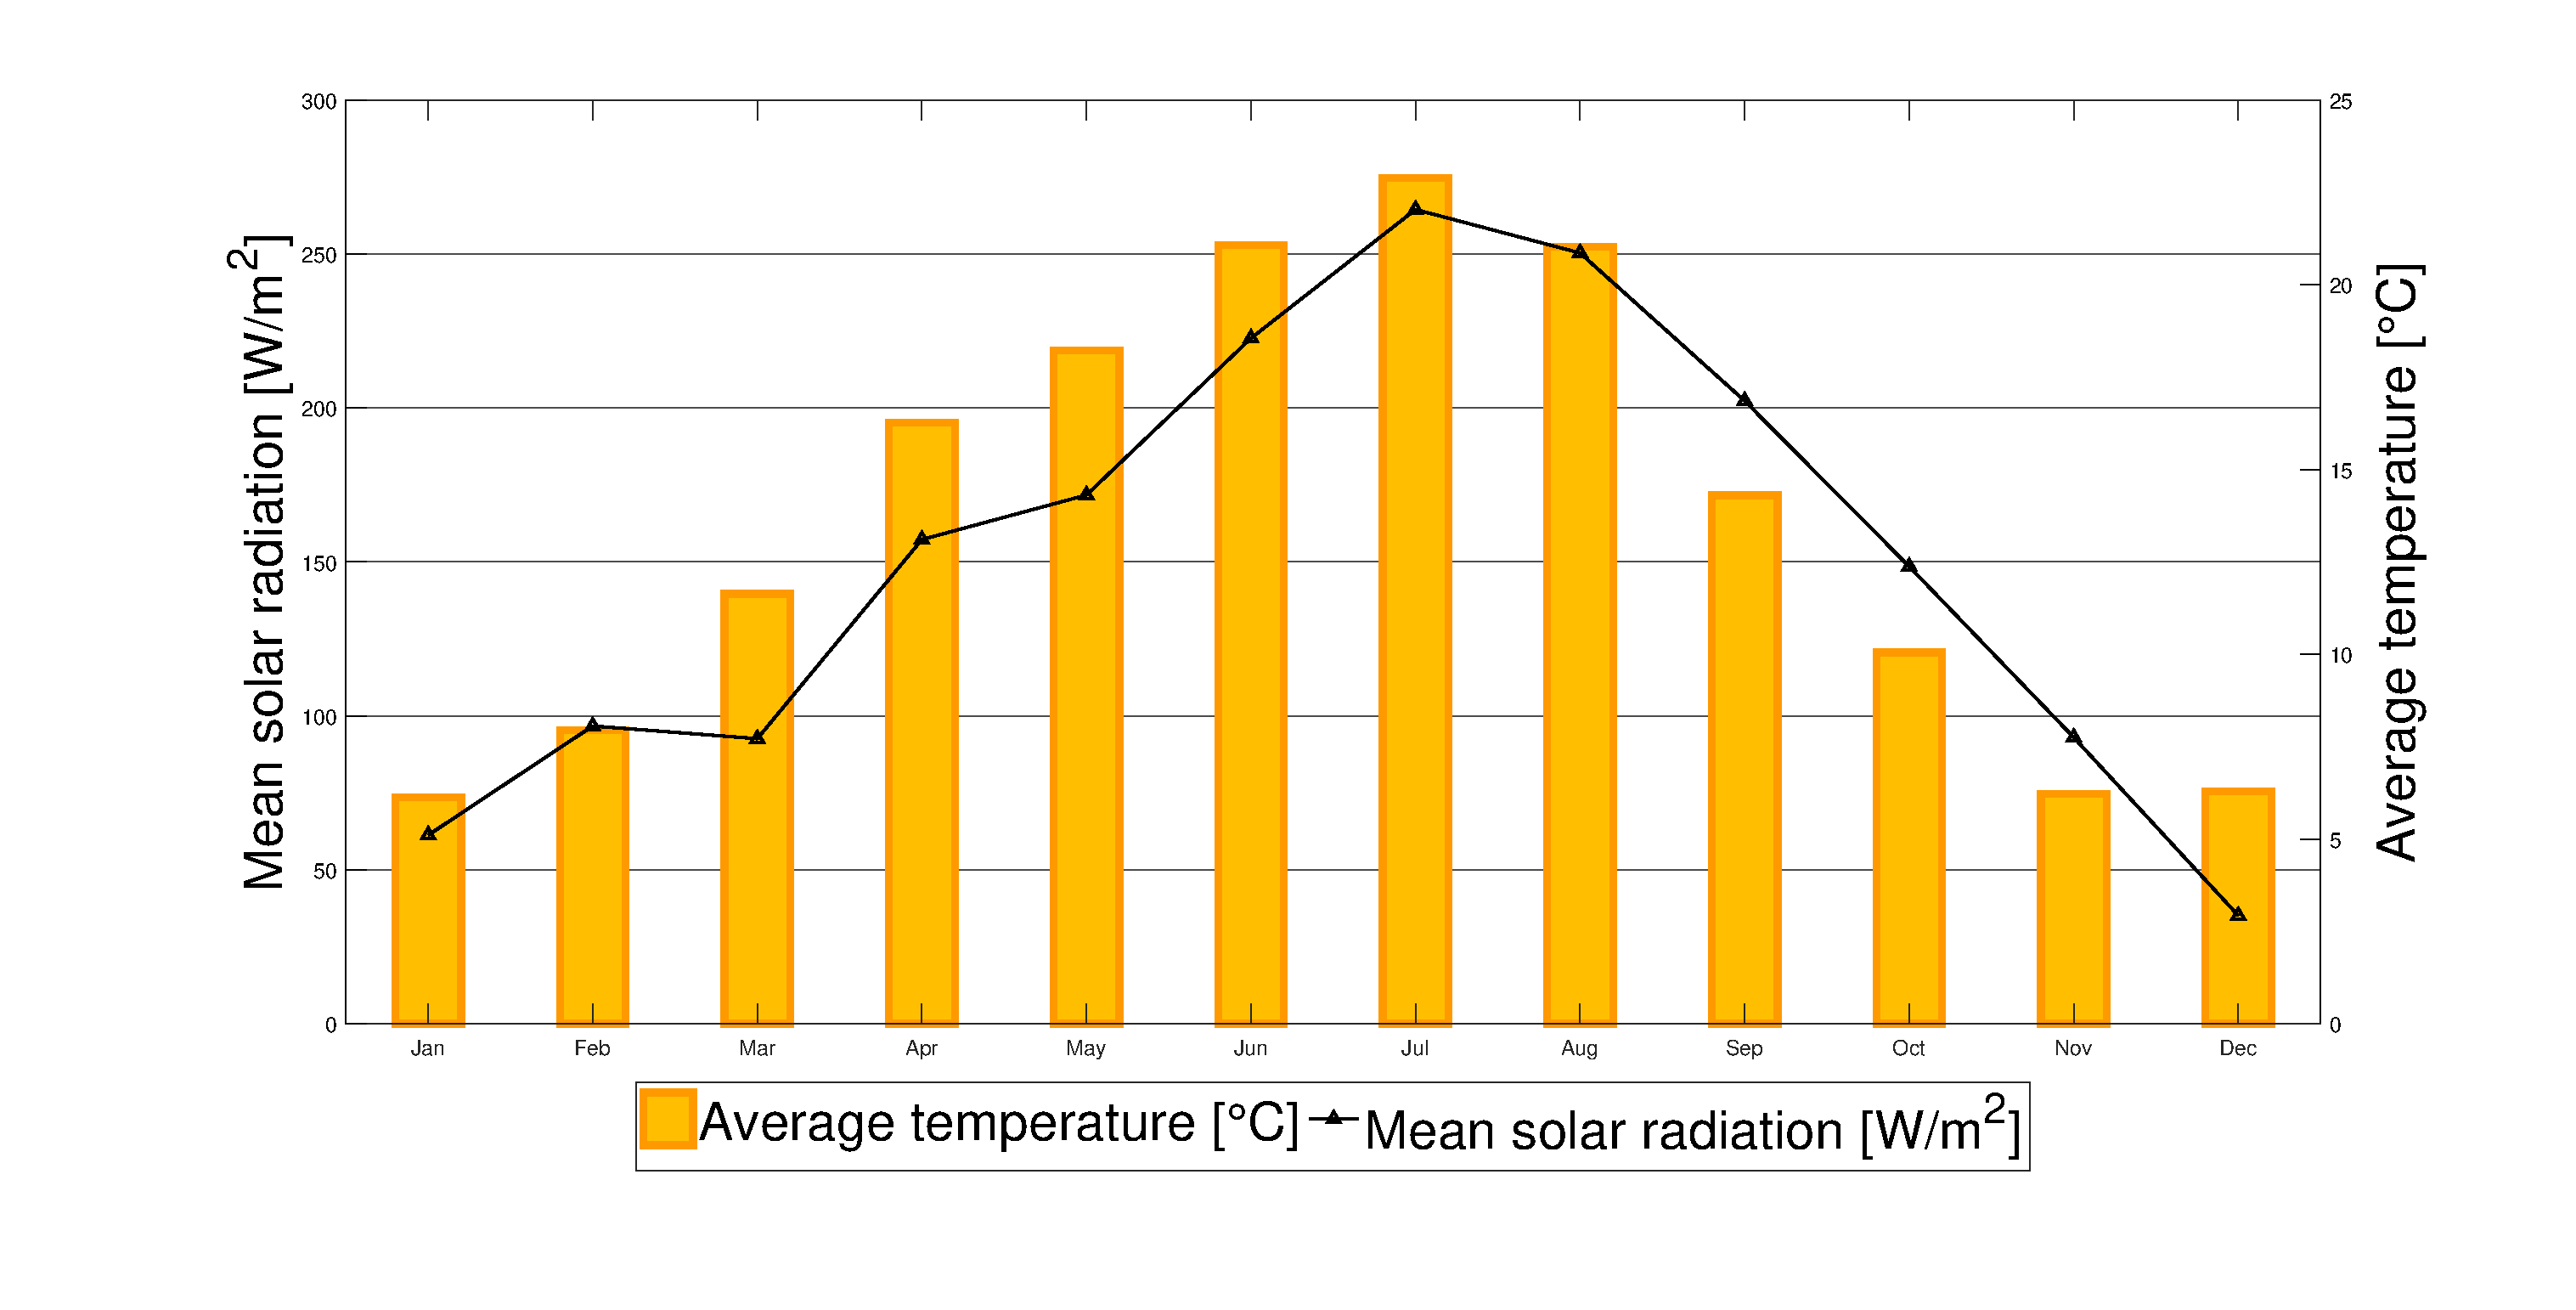
\includegraphics[width=28pc]{figures/dati_climatici_rev01.eps}
		\vspace{-0.5cm}
		\caption{Weather data of L'Aquila, Italy.}
		\captionsetup{justification=centering}
		\label{F:houseExternalWeather}
	\end{center}
\end{figure}
\begin{table}[t!]
	\centering
	\begin{tabular}{ccccc}
		\toprule
		\multirow{3}{1.4cm}{\centering Structural member} & \multirow{3}{3.7cm}{\centering Layer 
			description (from inside to outside)}       & Thermal     		     & Total     & Total        \\
		&                                             & resistance   		     & thickness & U-value      \\
		&                                             & $[(m^2K)/W]$		     & $[m]$     & $[W/(m^2K)]$ \\
		
		
		\midrule
		\multirow{3}*{Wall}                               & Wood-cement                                 & $0.308$     		     &           &              \\ 
		& Concrete                                    & $0.096$    		     & $0.50 $   & $0.12 $      \\ 
		& EPS and graphite                            & $6.774$    		     &           &              \\
		&							                    &						 &		     &			    \\
		
		
		\multirow{3}*{Floor}        					  & Wood-cement                                 & $0.308$     		     &           &              \\ 
		& Polystyrene                                 & $6.000$     		     & $0.23 $   & $0.28 $      \\ 
		& Screed                                      & $0.027$     		     &           &              \\
		&									    	    &					 	 &		     &			    \\
		
		
		\multirow{5}{1.4cm}{\centering Pitched roof} 	  & Wood-cement                                 & $0.308$                &           &              \\ 
		& Polystyrene                                 & $6.000$                &           &              \\
		& Screed                                      & $0.027$                & $0.31 $   & $0.13 $      \\ 
		& \multirow{2}{3.7cm}{\centering Polyurethane 
			resins and polyisocianurate foams}          & \multirow{2}*{$4.000$} &           &              \\
		&                                             &                        &           &              \\
		\bottomrule
	\end{tabular}
	\caption{Wood-cement blocks properties.}
	\captionsetup{justification=centering}
	\label{T:houseProperties}
\end{table}
In order to calibrate the EnergyPlus model, a comparison between simulated and measured thermal energy consumption was performed. Considering the off-grid characteristic of the house, the installation of a heat meter was necessary for acquiring the actual energy consumption. Moreover, the heat meter installation has allowed a detailed knowledge of the actual heating system scheduling, shown in Figure \ref{F:houseActualScheduling}, faithfully reproduced in the simulated model. The heat meter, that consists of two thermocouples for flow and return thermal fluid temperatures, a turbine flowmeter and a controller, employed Equation \eqref{Eq:energyConsumption} to calculate the real thermal energy consumption $\dot Q$ of the house.
\begin{equation}\label{Eq:energyConsumption}
\dot Q = 0.2777698\times10^{-3}\times\rho\times\Delta V\times c_p\times\Delta T
\end{equation}
In \eqref{Eq:energyConsumption} $\dot Q$ is the thermal energy consumption $[Wh]$, $\rho$ is the water density $[kg/m^3]$, $\Delta V$ is the water volume variation $[m^3]$ detected by the turbine flowmeter, $c_p = 4.186\, [kJ/(kgK)]$ is the water specific heat at constant pressure, $\Delta T$ is the difference between flow and return temperatures of the water $[K]$, $0.2777698∙10−3$ is a dimensionless conversion factor. The considered period goes from March $15$, $2016$ to April $15$, $2016$.
\begin{figure}[t!]
	\begin{center}
		\includegraphics[width=20pc]{figures/Render_rev01.eps}
		\caption{Virtual model of the use case.}
		\captionsetup{justification=centering}
		\label{F:houseVirtualModel}
	\end{center}
\end{figure}
\begin{figure}[t!]
	\begin{center}
		\includegraphics[width=28pc]{figures/Scheduling_rev02.eps}
		\caption{Actual scheduling of the heating system, where white color means switched OFF and green color switched ON, and ($T_{ext,ave}$) is the external average temperature. From midnight to $8am$ the heating system is always switched off.}
		\captionsetup{justification=centering}
		\label{F:houseActualScheduling}
	\end{center}
\end{figure}
Following the hourly calibration proposed by the M\&V guidelines of ASHRAE \cite{USDOE}, also applied in \cite{Mustafarai2014,Raftery2011}, a simulated model is calibrated when the mean bias error (MBE) and the coefficient of variation of the root mean square error [CV(RMSE)] are less than acceptable tolerances, respectively equal to $\pm 10.0\%$ and $30.0\%$. MBE and CV(RMSE) have been calculated by using Equations \eqref{Eq:mbe} and \eqref{Eq:cvrmse}.

\begin{equation}\label{Eq:mbe}
MBE(\%) = \frac{\sum_{Period}{(S-M)_{Interval}}}{\sum_{Period}{M_{Interval}}} \times 100
\end{equation}

where $M$ is the measured $kWh$ and $S$ is the simulated $kWh$.

\begin{align}\label{Eq:cvrmse}
\nonumber CV(RMSE_{Period}) &= \frac{RMSE_{Period}}{A_{Period}} \times 100 \\
				            &= \sqrt{\frac{\sum{(S-M)^2_{Interval}}}{N_{Interval}}} \times \frac 1{A_{Period}} \times 100
\end{align}

where $A_{Period}$ is the mean of the measured data for the period, Equation \eqref{Eq:aperiod}, and $N_{Interval} = 4563$ is the number of time intervals in the monitoring period.

\begin{equation}\label{Eq:aperiod}
A_{Period} = \frac{\sum_{Period}{M_{Interval}}}{N_{Interval}}
\end{equation}

The comparison between numerical and experimental data is shown in Figure \ref{F:houseComparisonExperimental} and shows a quite good agreement. Therefore, with a MBE equal to $7.38\%$ and a CV(RMSE) equal to $8.37\%$, the EnergyPlus model of the use case can be considered well calibrated.  
\begin{figure}[t!]
	\begin{center}
		\subfigure[Thermal energy comparison. The accuracy error is $7.38\%$ with MBE definition and $8.37\%$ with CV(RMSE) definition]{
			\label{F:houseComparisonExperimentalEnergy}
			\centering
			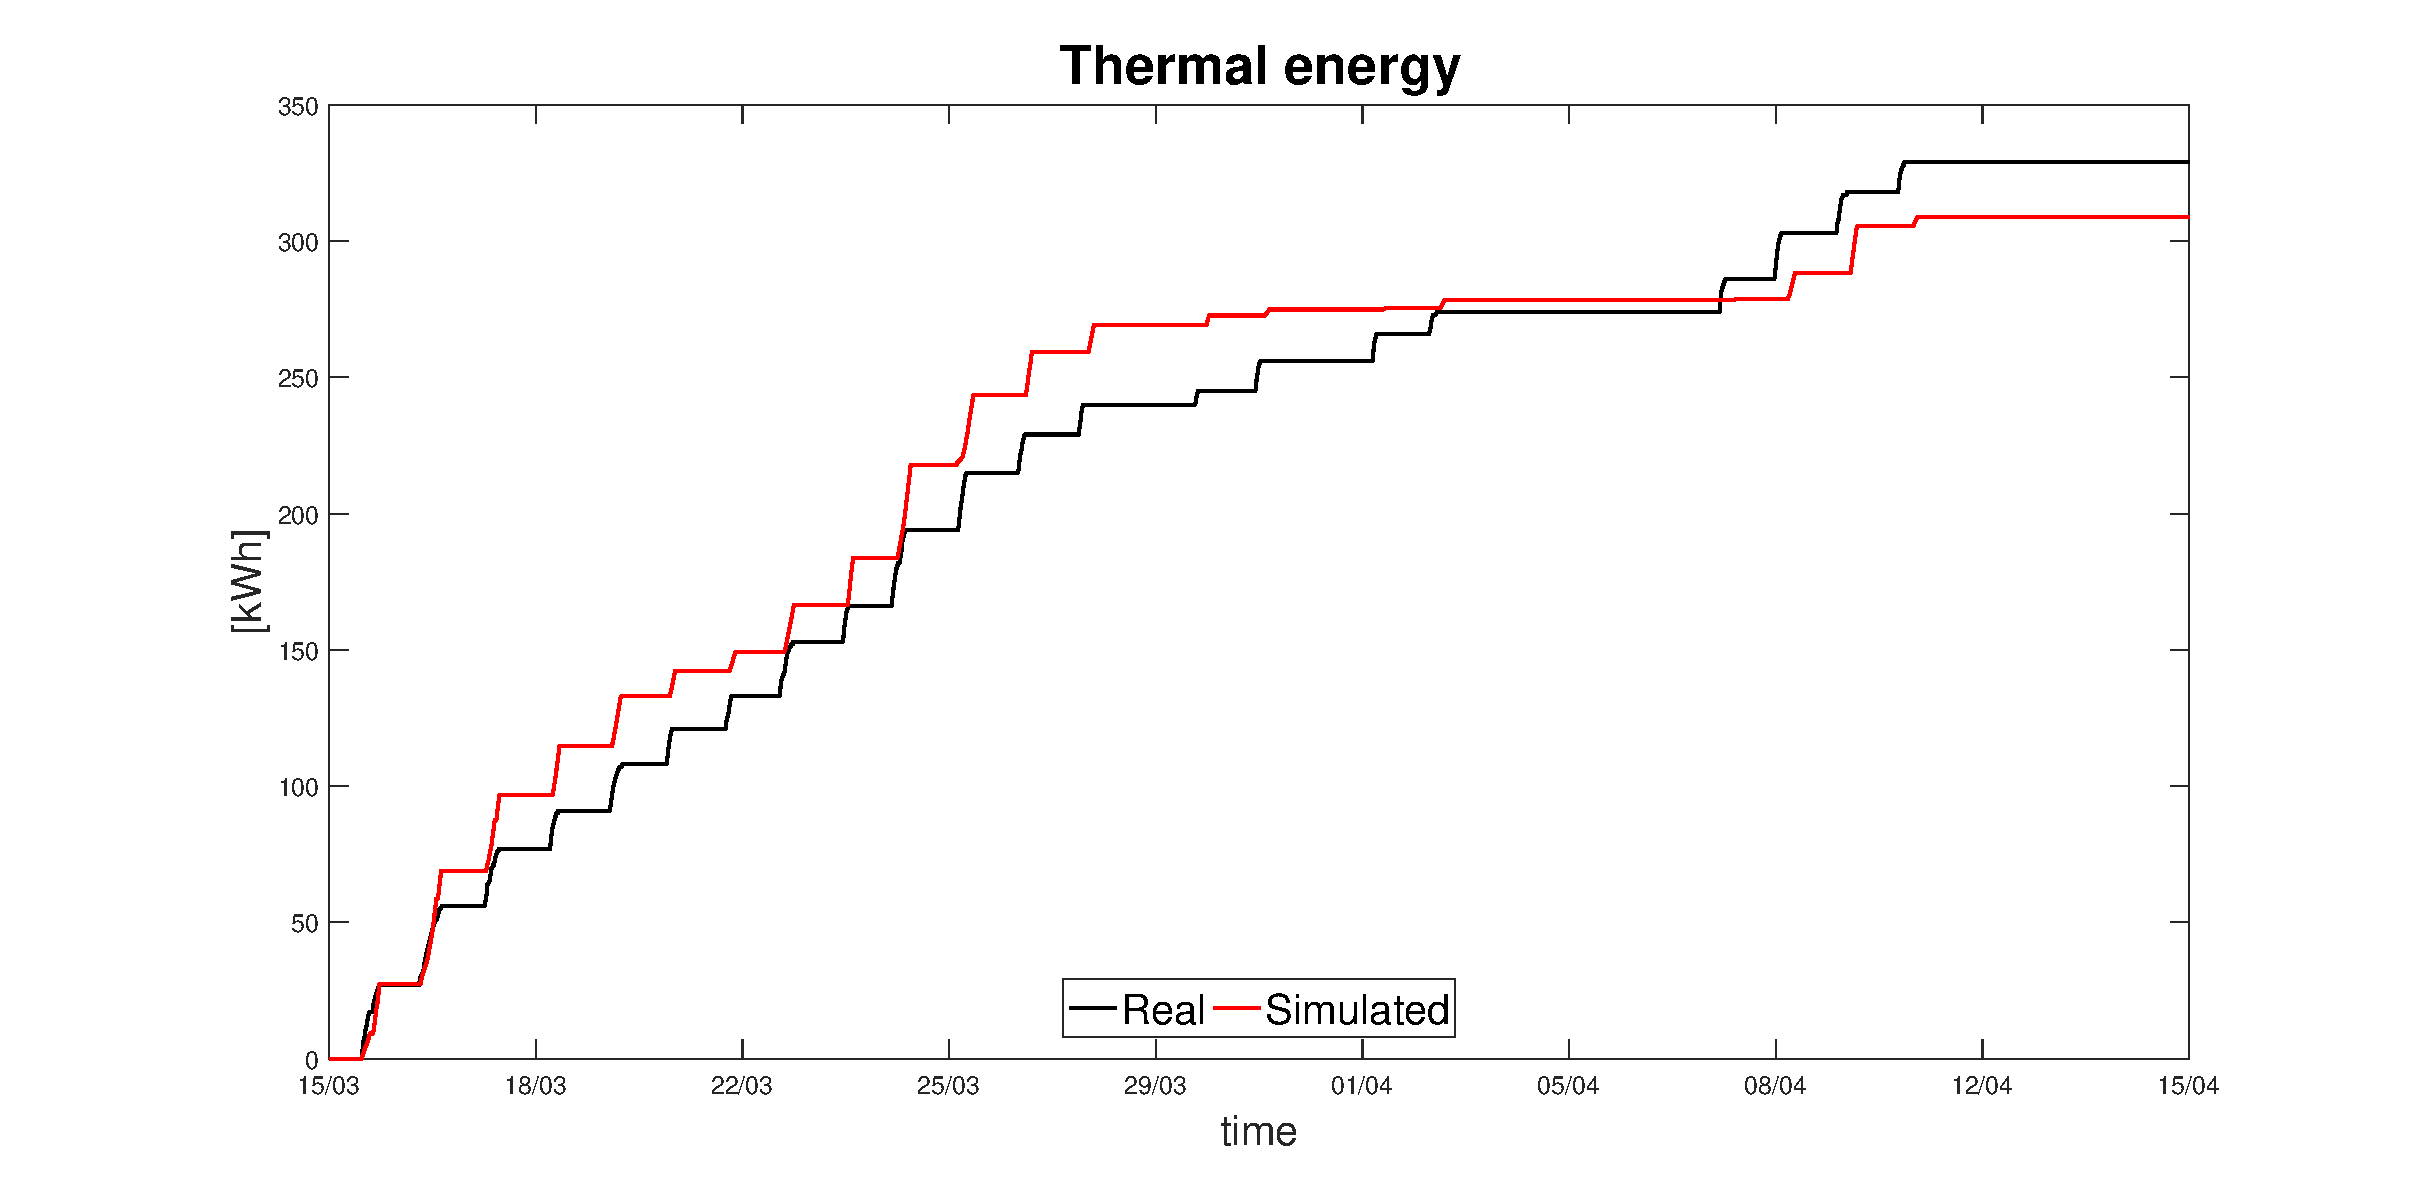
\includegraphics[width=28pc]{figures/Thermal_energy_rev01.eps}
		}
		\subfigure[Thermal power comparison.]{
			\label{F:houseComparisonExperimentalPower}
			\centering
			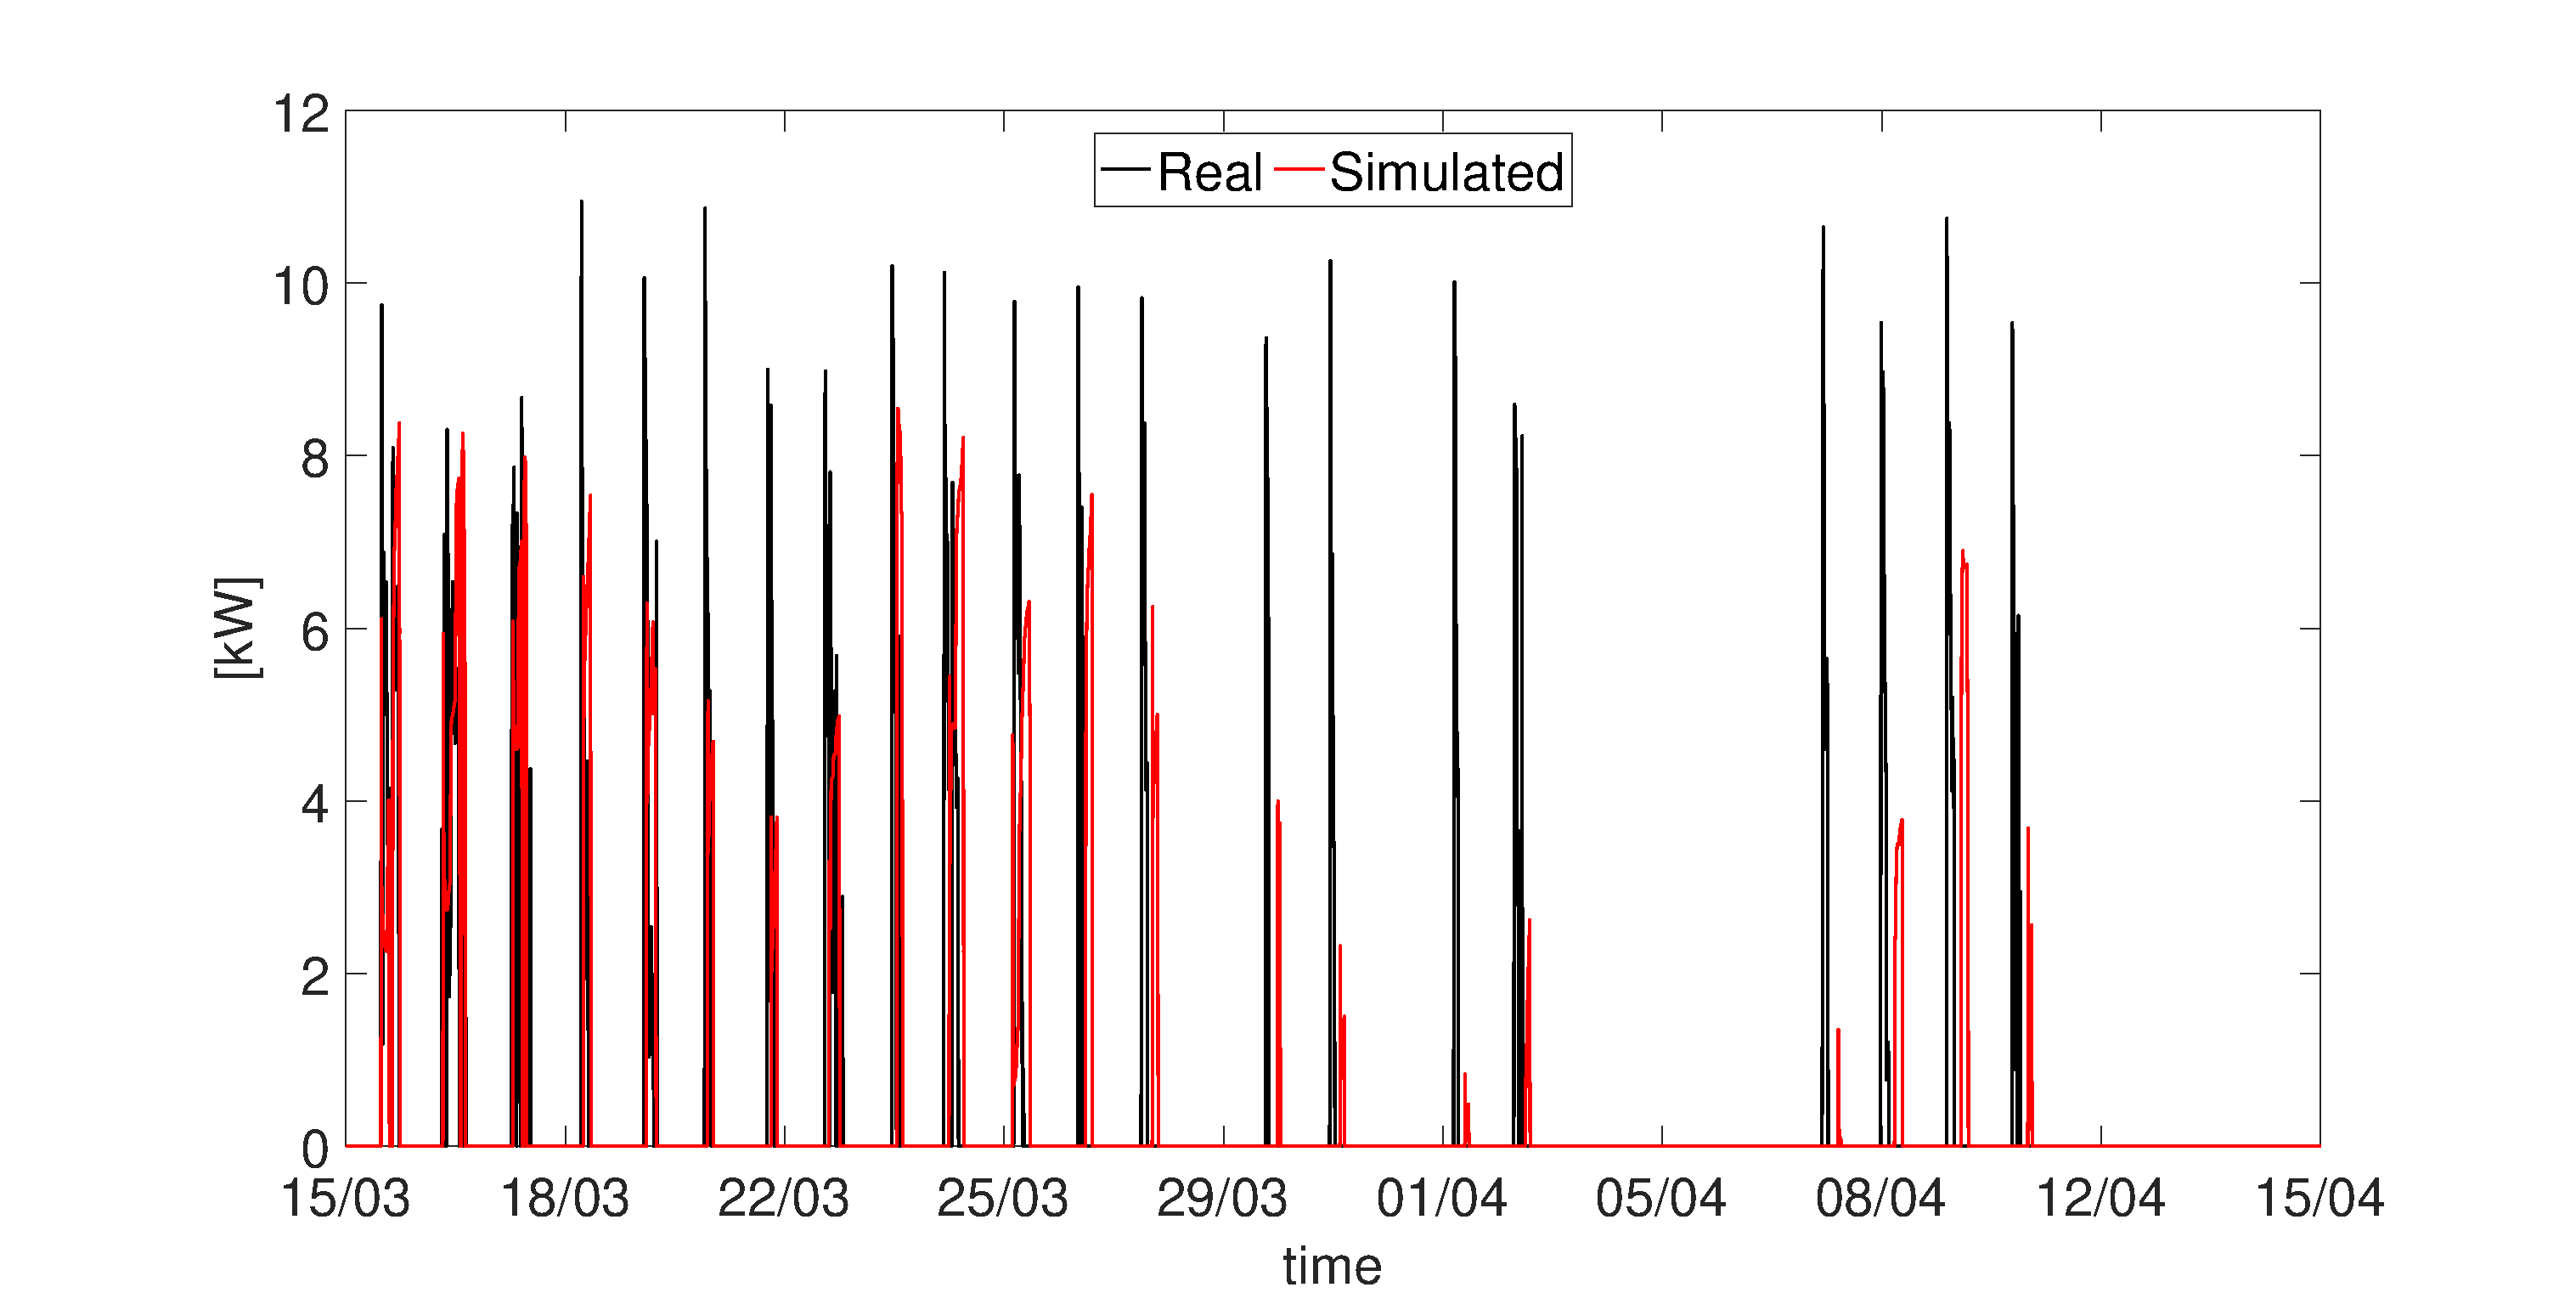
\includegraphics[width=28pc]{figures/Thermal_power.eps}
		}
	\end{center}
	\caption{Comparison between numerical and experimental data.}
	\captionsetup{justification=centering}
	\label{F:houseComparisonExperimental}
\end{figure}
\subsection{Random forest models}
\label{SS:randomForestsModels}
For the closed-loop simulations with DPC we create $2$ different sets of models, $S_1 = \{\tT^{r_1}_{\mathrm{k+1|k}},\tT^{r_2}_{\mathrm{k+1|k}},\tT^{r_3}_{\mathrm{k+1|k}},\tT^{r_4}_{\mathrm{k+j|k}}\}$ and $S_2 = \{\tP_{\mathrm{k+j|k}},\tT^{1}_{\mathrm{k+j|k}},\tT^{2}_{\mathrm{k+j|k}},\tT^{3}_{\mathrm{k+j|k}},\\\tT^{4}_{\mathrm{k+j|k}},\ j = 1,\ldots,N\}$, using random forests. In each set we have  $4$ models that describe the room temperature evolution ($\tT^{r_i}$ and $\tT^i$, $i=1,2,3,4$) in each of the $4$ rooms equipped with temperature sensors. In $S_2$ we have a model for the power consumption of the house ($\tP$). Models in $S_1$ are created using the classical random forests algorithm with all the features and are used as plant simulator of the house. For this reason, they are computed to give prediction only for time step $k+1$ and not over the whole horizon $N$. Models in $S_2$ are used as predictors over a horizon $N$ in the DPC algorithm and are then created using the methodology provided in Section \ref{SS:dpcrf}. The non-manipulated features in $\tX^d$ are the disturbance data (relative humidity, atmospheric pressure, outside air temperature, solar radiation, wind, time of the day and day of the week) and the states (temperature of the $4$ rooms). The manipulated feature in $\tX^c$ is the flow rate ($[m^3/h]$). All this features are used to create models in $S_1$ and the power model in $S_2$, while disturbance data, state temperature of room $i$ only and flow rate are used to identify $\hat{\Theta}^{T}_{\tT^i_j}$ for temperature models in $S_2$. All the models have been trained on the data from March $11$, $2016$ to April $26$, $2016$ and validated on the data from May $1$, $2016$ to May $15$, $2016$. The accuracy of these models with respect to real data is shown in Table \ref{T:S1accuracy}, based on the definition of Normalized Root Mean Square Error (NRMSE).

A graphical comparison is shown in Figure \ref{F:power_testing} for the power consumption and Figure \ref{F:temperature_testing} for the temperature of room $1$. The plots for the other rooms are omitted since they are very similar.


%We use random forest model $\tP^r$ also to estimate the energy consumption of the house. In particular we estimated it for the same period analyzed in Section \ref{SS:energyPlusmodel} and obtained the results in Figure \ref{F:Energy_testing}, with a MBE equal to $13.0\%$ and a CV(RMSE) equal to $13.7\%$.
%
%\begin{figure}[h!]
%	\begin{center}
%		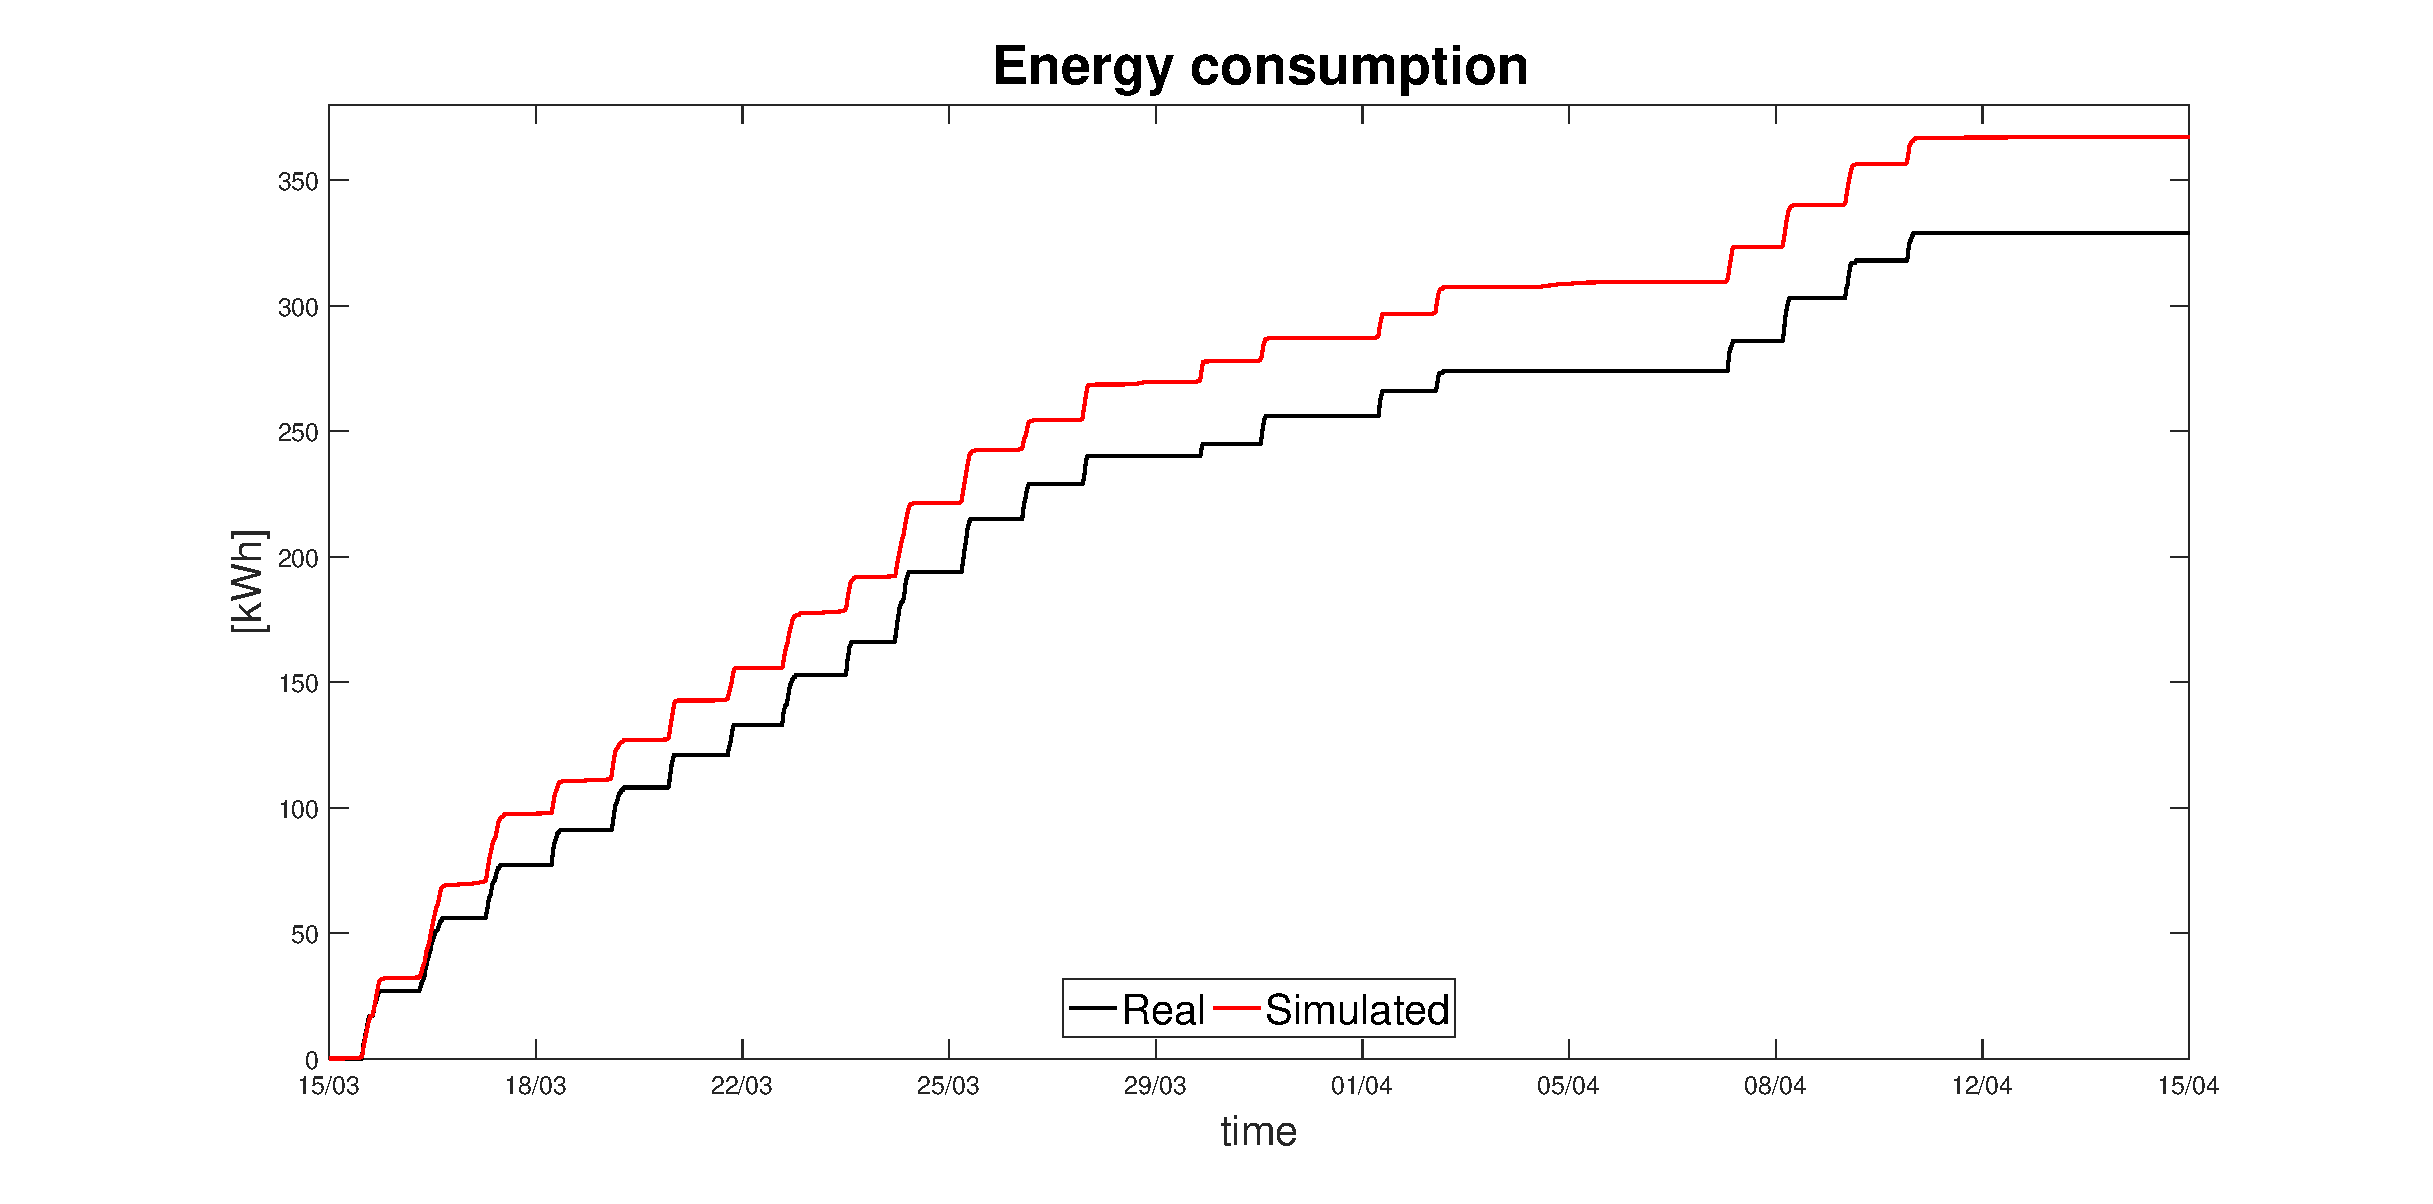
\includegraphics[width=26pc]{figures/Energy_test.eps}
%		\caption{Energy consumption accuracy.}
%		\captionsetup{justification=centering}
%		\label{F:Energy_testing}
%	\end{center}
%\end{figure}
%
%As we can see, with random forest model we get a worse MBE and CV(RMSE) for energy consumption, although the maximum error is very similar. This is because the EnergyPlus model, due to its internal dynamics based on the house structure, is able to compensate the error over time. On the other hand our curve perfectly follows the time behavior of the real case. For this reason, in Section \ref{SS:simulationResults}, we will use both models in order to compare the quality of the DPC with respect to a classical bang-bang controller.

\subsection{DPC and bang-bang controllers}
\label{SS:controllersDPCandBangbang}
We set up $2$ different controllers, DPC and bang-bang controller, to obtain a scheduling policy to switch the radiators ON and OFF in order to keep the temperature of room $3$, i.e. the living room, within a comfort range. Since the heating system serves all of the $4$ rooms simultaneously, without giving the possibility to control the temperature of each room independently, we setup the problem defining the comfort range only for one room. Other rooms temperatures will follow the scheduling policy. Room $3$ has been chosen randomly. In the following we describe the $2$ controllers.

\paragraph{DPC}
We want to optimize the ON/OFF heating system schedule in order to minimize power consumption of the house while keeping temperature of room $3$ within a comfort range. We also allow violations $\eps^{min},\eps^{max}$  of temperature bounds to guarantee feasibility of the algorithm. We include these violations in the objective function to be minimized.
\begin{table}[t!]
	\centering
	\begin{tabular}{cccccc}
		\toprule
		Set       & Power   & T. room $1$ & T. room $2$ & T. room $3$ & T. room $4$  \\ 
		\midrule
		$S_1$     &         & $96.58$     & $96.99$     & $97.21$     & $96.62$\\
		$S_2$     & $92.21$ & $97.38$     & $97.29$     & $96.93$     & $96.81$\\
		\bottomrule
	\end{tabular}
	\caption{Models accuracy for power and temperatures models in $S_1$ and $S_2$ expressed as $\mathrm{1-NRMSE}\,(\%)$.}
	\captionsetup{justification=centering}
	\label{T:S1accuracy}
	\vspace{-0.5cm}
\end{table}
\begin{figure}[t!]
	\begin{center}
		\subfigure[Power consumption model accuracy validation. The accuracy over the testing period expressed as $\mathrm{1-NRMSE}\,(\%)$ is $92.1\%$.]{
			\label{F:power_testing}
			\centering
			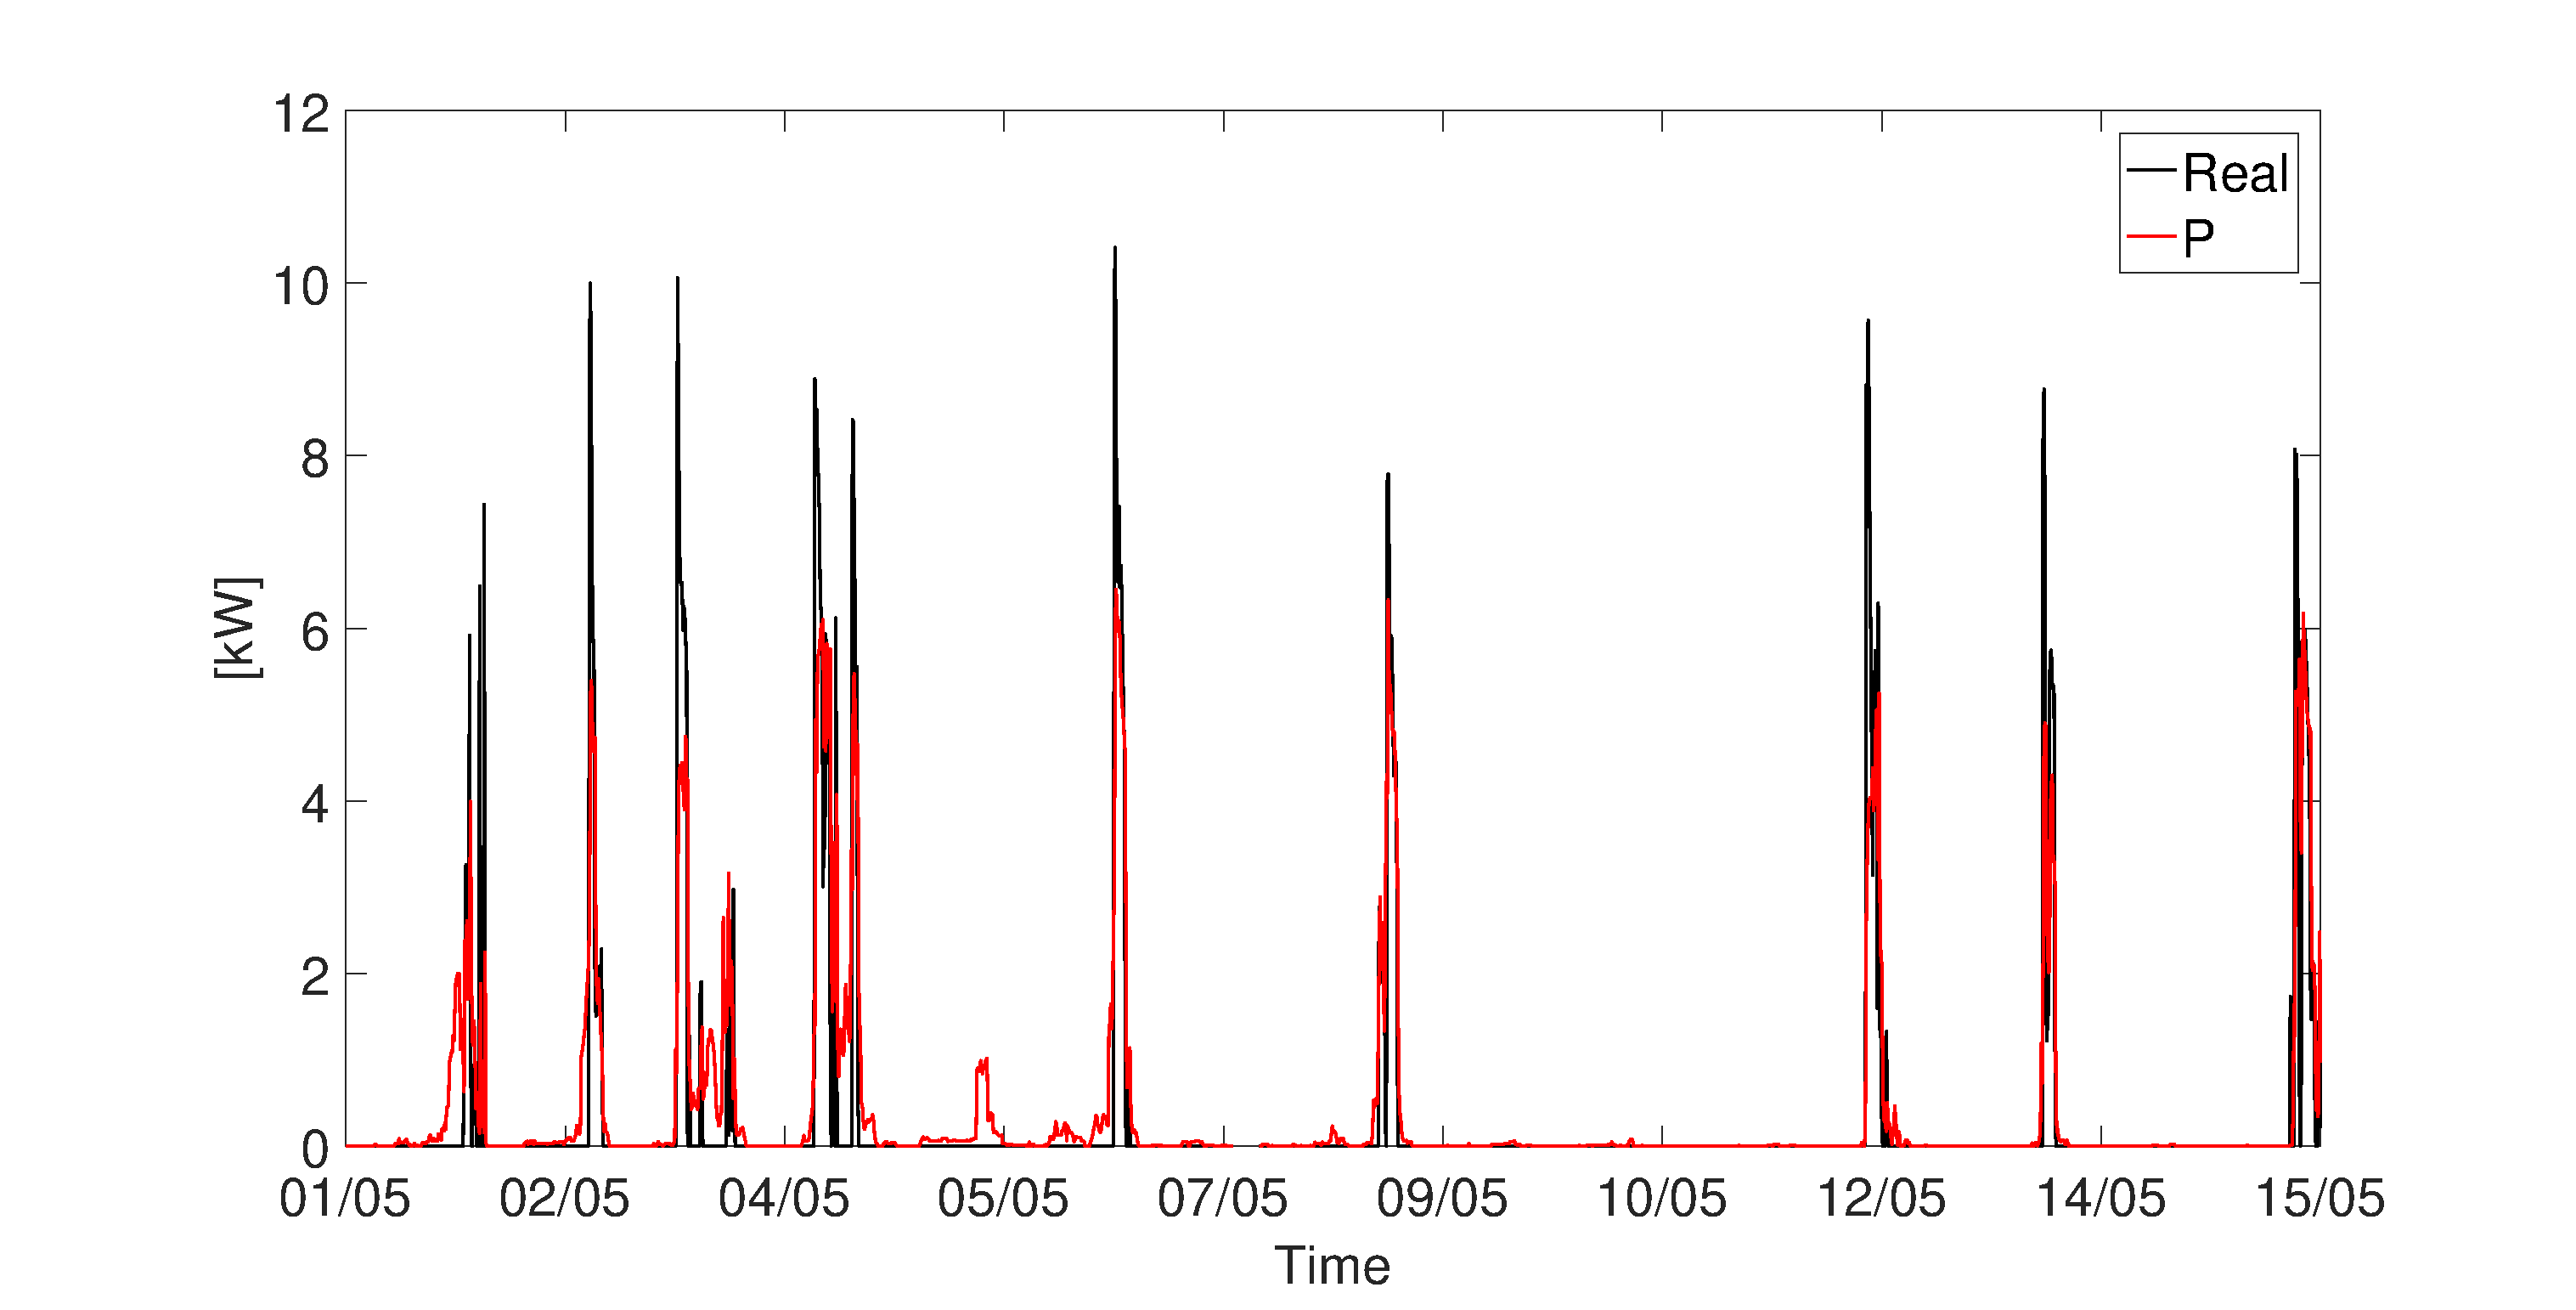
\includegraphics[width=26pc]{figures/power_testing.eps}
		}
		\subfigure[Temperature model accuracy validation for room $1$. The accuracy over the testing period expressed as $\mathrm{1-NRMSE}\,(\%)$ is $96.58\%$, for the temperature model $T^{r_1}$ in $S_1$ and $97.3\%$ for the temperature model $T^1$ in $S_2$. The accuracy for the other rooms is very similar as can be seen in Table \ref{T:S1accuracy}.]{
			\label{F:temperature_testing}
			\centering
			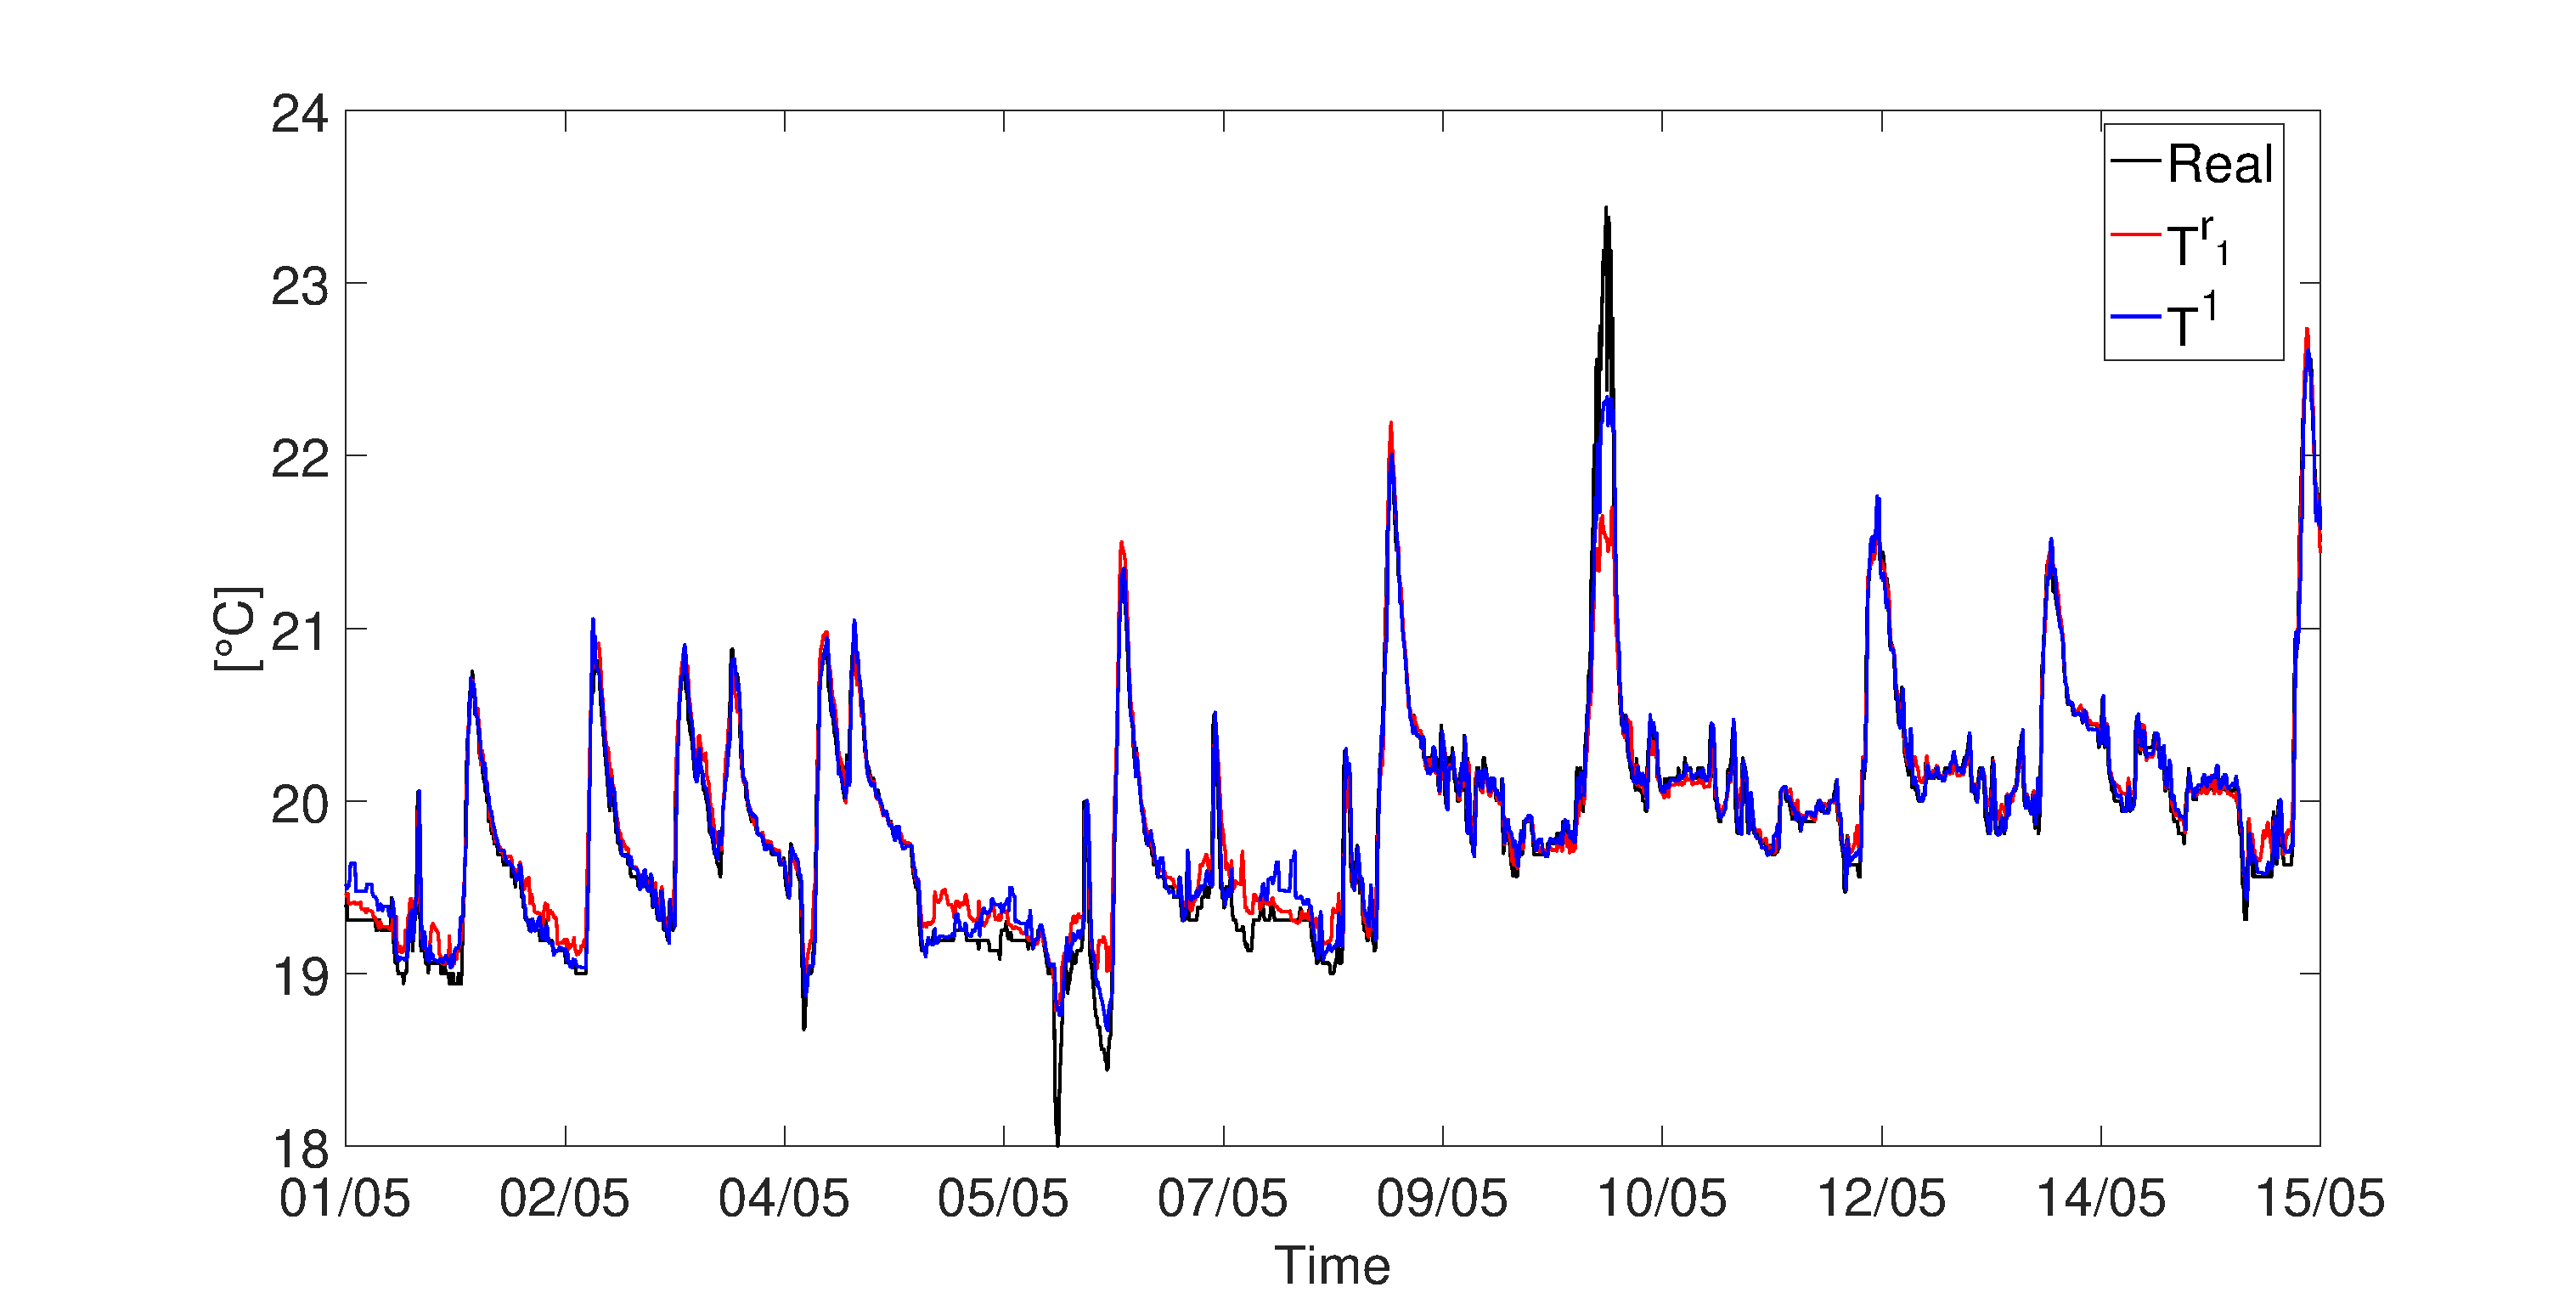
\includegraphics[width=26pc]{figures/temperature_testing.eps}
		}	
	\end{center}
	\vspace{-0.7cm}
	\caption{Model accuracy validation for power and temperature models.}
	\vspace{-0.7cm}
	\captionsetup{justification=centering}
	\label{F:testing}
\end{figure}

The problem is set up as follows:
\begin{problem}\label{P:dpcRealCase}
\begin{align}
	\begin{aligned}
		\min_{\tX^c,\eps_j^{min},\eps_j^{max}} & \ \ \ \sum_{j=1}^{N} Q{\tP}_{\mathrm{k+j|k}}^2 +  \lambda_{min}\parallel\eps^{min}\parallel_2 + \lambda_{max}\parallel\eps^{max}\parallel_2 \\
		\text{s.~t. }& \ \ \ \ \ {\tP}_{\mathrm{k+j|k}} =  \hat{\Theta}^{T}_{\tP_j} [ 1,\tX^c_{\mathrm{k|k}},\dots,\tX^c_{\mathrm{k+j-1|k}} ]^T \\
					 & \ \ \ \ \ \tT^1_{\mathrm{k+j|k}} =  \hat{\Theta}^{T}_{\tT^1_j} [ 1,\tX^c_{\mathrm{k|k}},\dots,\tX^c_{\mathrm{k+j-1|k}} ]^T \\
					 & \ \ \ \ \ \tT^2_{\mathrm{k+j|k}} =  \hat{\Theta}^{T}_{\tT^2_j} [ 1,\tX^c_{\mathrm{k|k}},\dots,\tX^c_{\mathrm{k+j-1|k}} ]^T \\
			 	 	 & \ \ \ \ \ \tT^3_{\mathrm{k+j|k}} =  \hat{\Theta}^{T}_{\tT^3_j} [ 1,\tX^c_{\mathrm{k|k}},\dots,\tX^c_{\mathrm{k+j-1|k}} ]^T \\
				 	 & \ \ \ \ \ \tT^4_{\mathrm{k+j|k}} =  \hat{\Theta}^{T}_{\tT^4_j} [ 1,\tX^c_{\mathrm{k|k}},\dots,\tX^c_{\mathrm{k+j-1|k}} ]^T \\					
					 & \underline{\tT}_{\mathrm{k+j-1|k}}-\eps^{min}_j \leq \tT^3_{\mathrm{k+j|k}} \leq \overline{\tT}_{\mathrm{k+j-1|k}} + \eps^{max}_j\\
					 & \ \ \ \ \ \ \ \ \tX^c_{\mathrm{k+j-1|k}} = \underline{\tX}^c \lor \tX^c_{\mathrm{k+j-1|k}} = \overline{\tX}^c\\ 
					 & \ \ \ \ \ \ \ \ \,\eps^{min}_j,\eps^{max}_j \geq 0, \ j = 1,\dots,N.
	\end{aligned}
	\label{E:DPCrealcase}
\end{align}
\end{problem}
The choice of different weights $Q$, $\lambda_{min}$ and $\lambda_{max}$ allows the designer to give more importance to energy consumption rather than temperature comfort and vice versa. In Section \ref{SS:simulationResults} we will show different performance results considering different weights. Parameters $\underline{\tX}^c$ and $\overline{\tX}^c$ are respectively minimum and maximum values the heating system can actuate, while $\underline{\tT}_{\mathrm{k+j-1|k}}$ and $\overline{\tT}_{\mathrm{k+j-1|k}}$ are respectively time varying lower and upper bounds to keep the temperature in a desired range of comfort. Due to the integer variable constraint for input $\tX^c$, the problem is a Mixed Integer Quadratic Programming. For the implementation we use in Section \ref{SS:simulationResults} Gurobi solver \cite{Gurobi2015} through CVX \cite{cvx,gb08}.

\paragraph{Bang-bang controller}
This is the classical controller widely used in private houses to keep temperature within a comfort range. It switches the heating system ON when the temperature goes under the temperature lower bound and switches it OFF when the temperature goes over the temperature upper bound. The advantage in using this controller is that it is very simple to set up. On the other hand it uses more energy than actually needed to achieve the task.

\subsection{Simulation Results}\label{SS:simulationResults} We simulated  DPC in \eqref{E:DPCrealcase} and the bang-bang controller, in closed-loop with the house models $\tT^{r_i}_{k+1|k},\ i=1,\ldots,4$ in $S_1$. We considered a sampling time of $10$ minutes and chose $N=4$ as a predictive horizon, i.e. $40$ minutes. From historical data we got that $\overline{\tX}^c = 0.35 \, m^3/h$ when the heating system is ON and obviously $\underline{\tX}^c = 0 \, m^3/h$ when the heating system is OFF. For the temperature comfort range we set a constant upper bound $\overline{\tT}_{\mathrm{k}} = 22.5 \, \degree C$ and a variable lower bound that is $\underline{\tT}_{\mathrm{k}} = 21 \, \degree C$ from $7am$ to $9am$ when people in the house wake up and go out for work, and from $6pm$ to midnight when people come back from work and go to sleep. During other hours when people are either not at home or asleep, we set $\underline{\tT}_{\mathrm{k}} = 20 \, \degree C$ 

We explained in Section \ref{SS:descriptionHouse} that the fuel used in the house is vegetable biomass. Therefore, it is not possible to have ON/OFF switching phases too close to each other, differently from a traditional gas boiler, due to the burning process and heat exchange. For this reason we set up both control problems with the constraint that when the heating system is activated it must stay active for at least $20$ minutes. This operating period can be obviously adapted depending on the fuel flow rate.

We ran DPC with $3$ different sets of parameters $Q$, $\lambda_{min}$ and $\lambda_{max}$. Each set allows a different level of temperature bounds violation. In particular, we considered a small ($Q=100$, $\lambda_{min}=3000$ and $\lambda_{max}=100$), a medium ($Q=100$, $\lambda_{min}=1000$ and $\lambda_{max}=100$) and a large ($Q=100$, $\lambda_{min}=100$ and $\lambda_{max}=100$) violation configuration.

\textcolor[rgb]{0,0,1}{We considered 2 different simulative conditions to show the robustness of our approach:
\begin{enumerate}
	\item in Section \ref{SSS:DisturbancePerfect} we provide our simulative results considering perfect knowledge of the weather forecast;
	\item in Section \ref{SSS:DisturbanceUncertain}, to show the robustness of our methodology, we consider weather forecast subject to uncertainty. We add a gaussian noise with high variance on the perfect forecast and show that the results are close to the perfect forecast case.
\end{enumerate}
\subsubsection{Perfect knowledge of the weather forecast}\label{SSS:DisturbancePerfect}
In this section we ran the simulations considering perfect knowledge of the disturbance over the horizon, obtaining the following results.}
\paragraph{Result 1} The comparison for temperature and input schedule obtained allowing small bound violations in DPC is shown in Figure \ref{F:comparison_small}. For sake of clarity, the simulation period is restricted to $4$ days and a half, from May $1$, $2016$ $00am$ to May $5$, $2016$ $1pm$. We can see that the temperature controlled with DPC does not violate the bounds and if it does then the violation is approximately $0.1\,\degree C$. Bang-bang control also presents small bounds violations due to its working principle. We can see how the DPC control law requires the heating system to be ON for less time than the bang-bang one to keep the temperature in the comfort range. 
We will see in Figure \ref{F:comparison_all_energy_E+} that this translates to significant energy saving.

\begin{figure}[t!]
	\begin{center}
	\subfigure[Temperature variation obtained with DPC and bang-bang controller.DPC controller allows almost no violation, so guaranteeing better comfort than bang-bang controller.]{
		\label{F:temperatures_small}
		\centering
		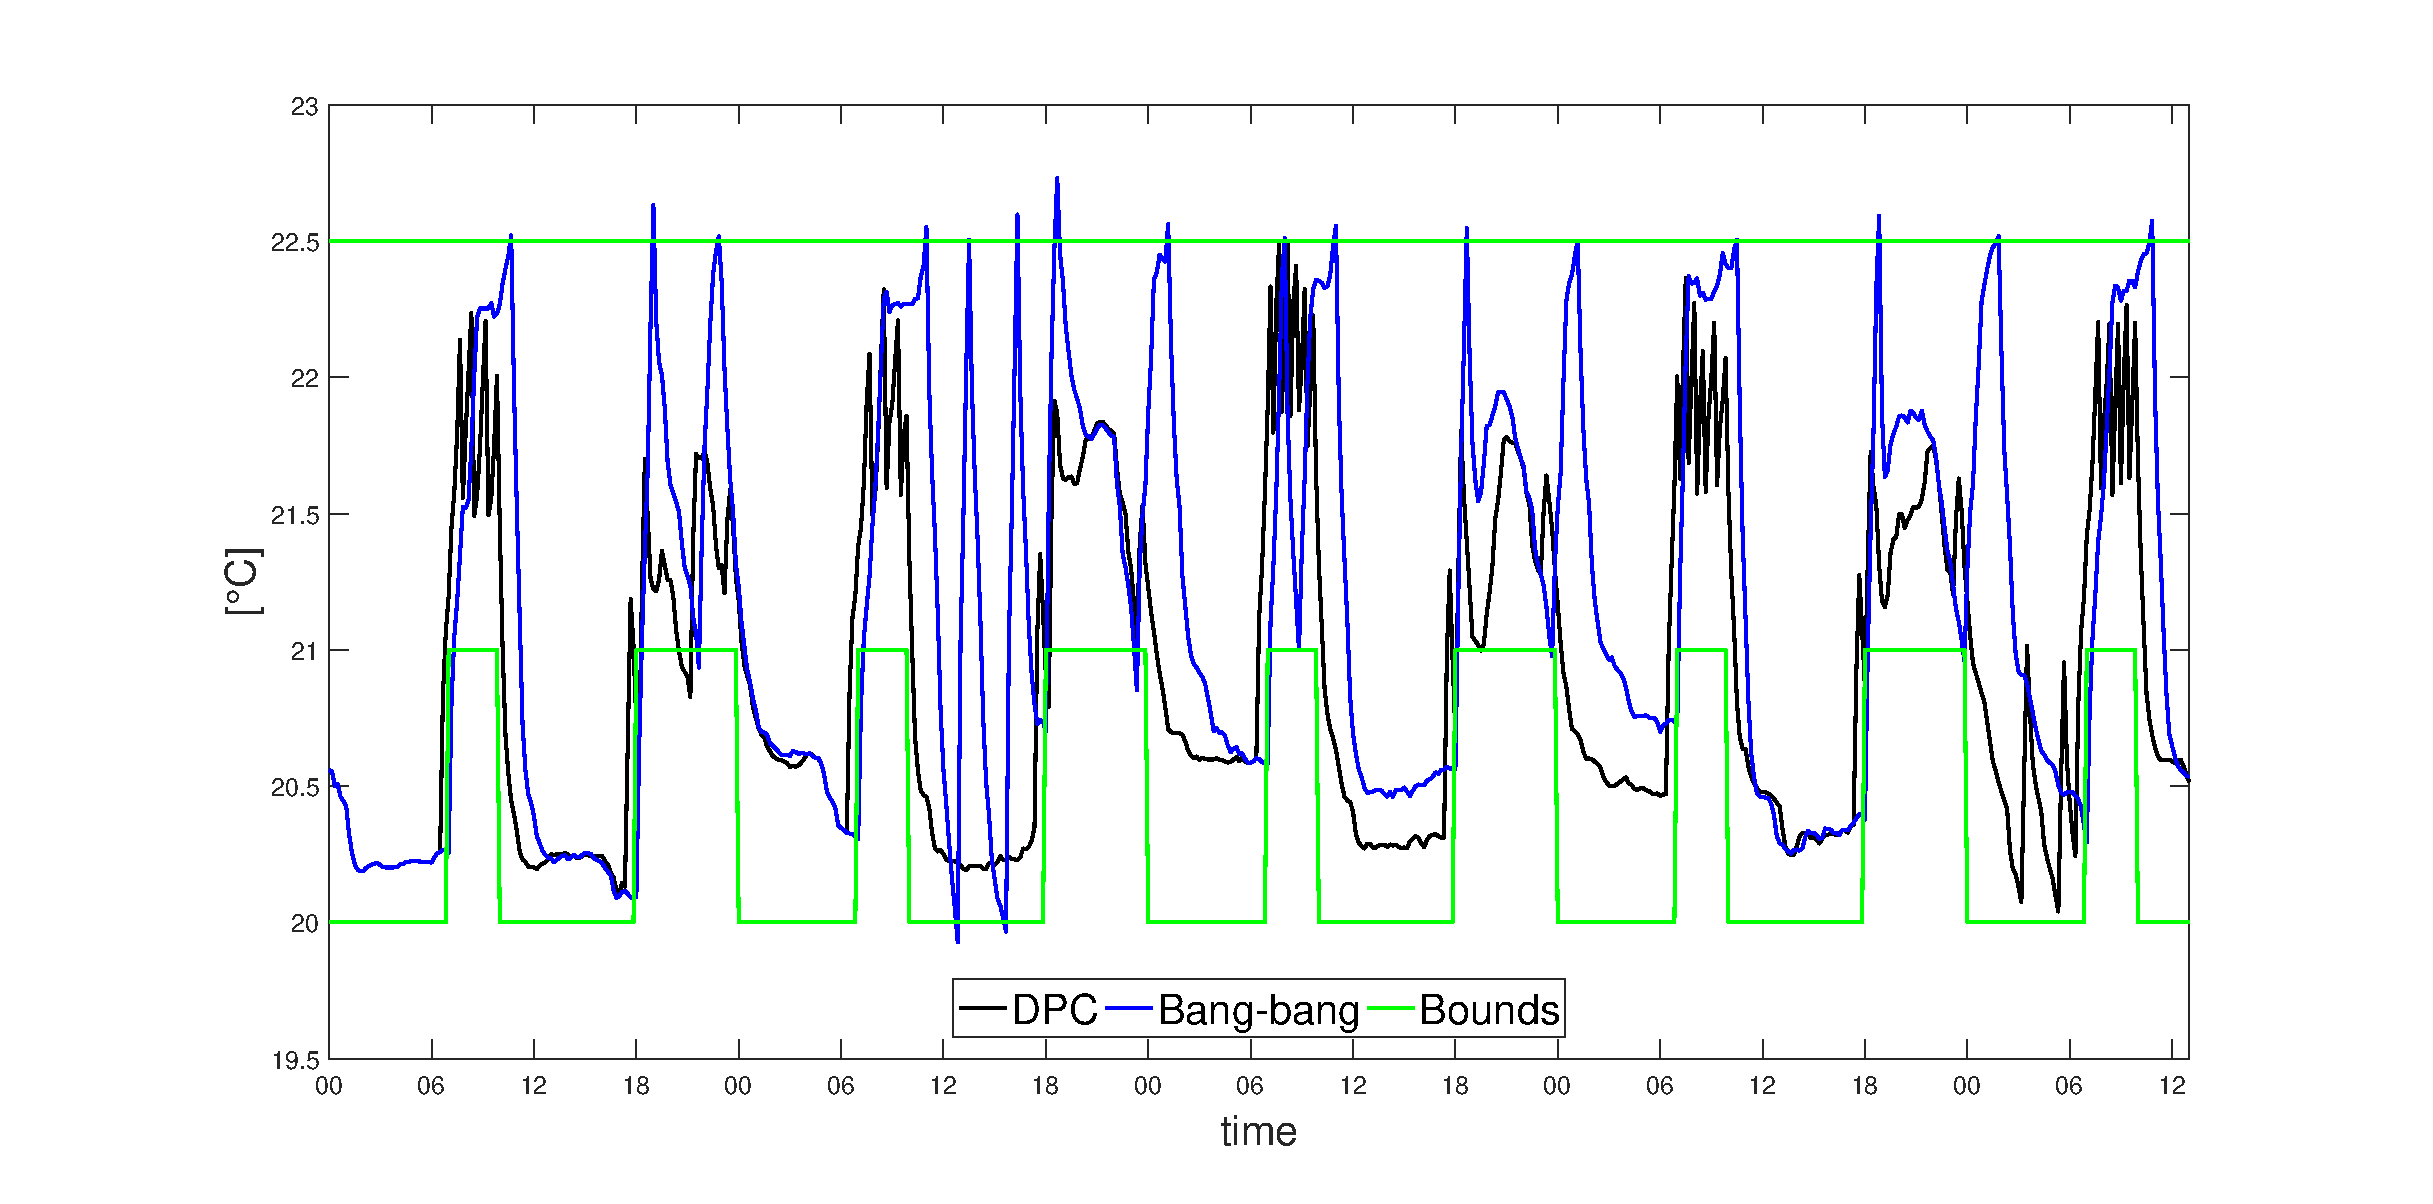
\includegraphics[width=28pc]{figures/Temperatures_small.eps}
	}
	\subfigure[Input schedules obtained from DPC and bang-bang controller. DPC keeps the heating system ON for less time than bang-bang controller, hence saving energy, and guarantees better thermal comfort.]{
		\label{F:inputs_small}
		\centering
		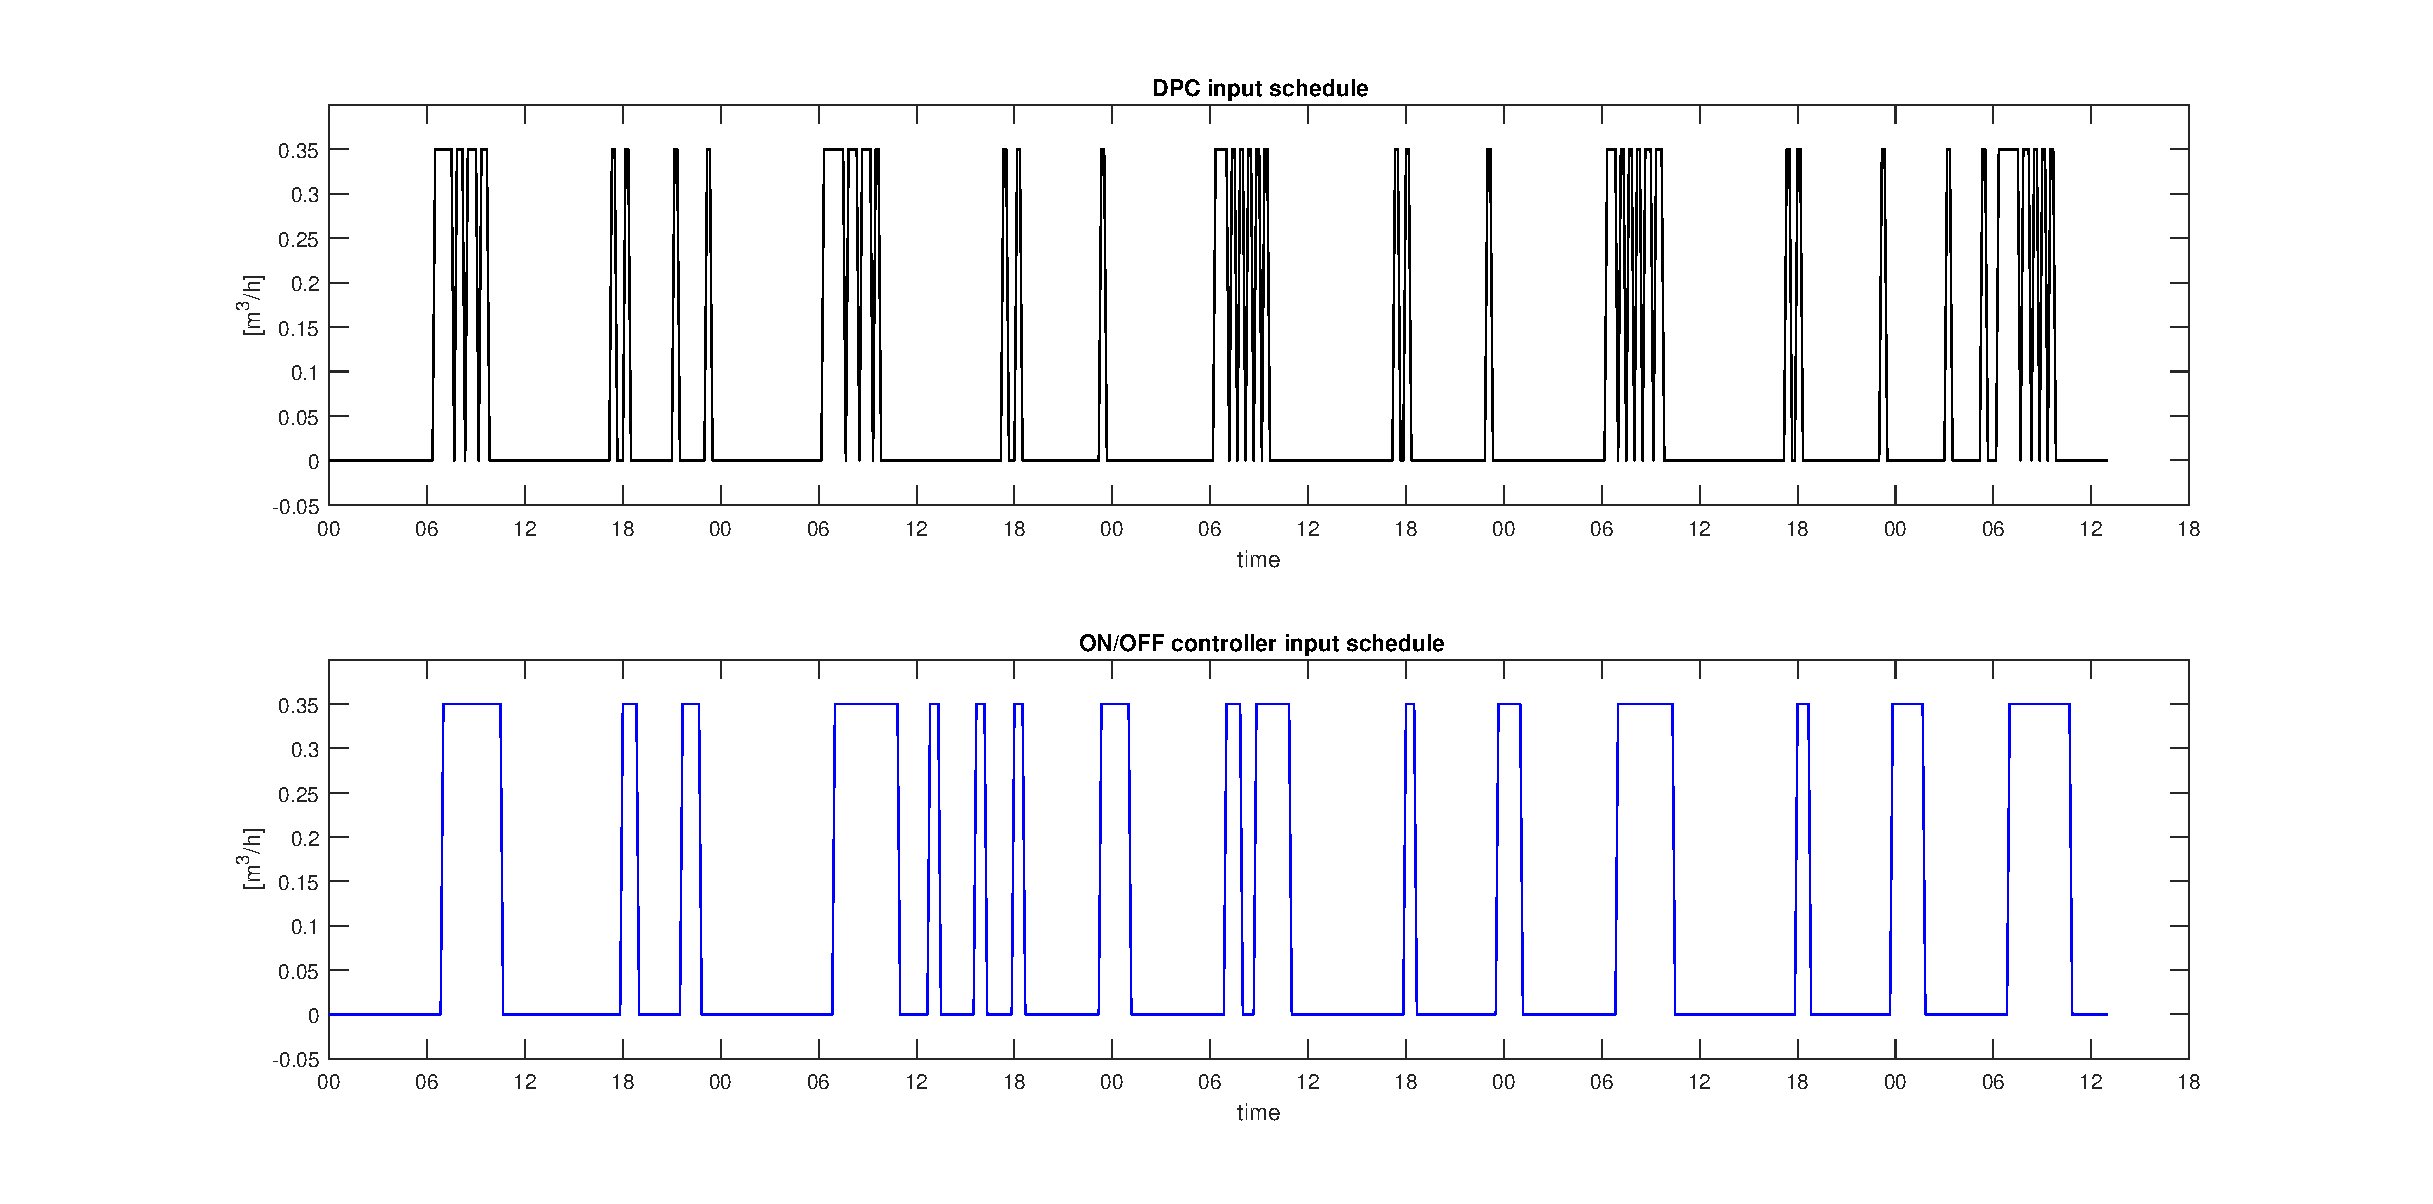
\includegraphics[width=28pc]{figures/Inputs_small.eps}
	}
	\end{center}
\vspace{-0.5cm}
	\caption{Comparison of DPC and bang-bang control performance over $5$ days of the testing period for room $3$.}
	\captionsetup{justification=centering}
	\label{F:comparison_small}
\end{figure}

\paragraph{Result 2} A comparison of temperature regulation obtained running the DPC with small, medium and large violations is shown in Figure \ref{F:comparison_all_temperature}. The results show that with the large violation configuration, that gives more importance to the power consumption minimization than to keep temperature within the bounds, temperature is almost always outside the lower bound during the period when the range is tighter. However the maximum violation is still lower than $1\,\degree C$.
In Table \ref{T:violationErrors}, MBE and CV(RMSE) violation errors are reported to quantify the bounds violation of DPC, in each of the $3$ configurations, and of bang-bang controller. We can see that if we allow very small violations, DPC outperforms bang-bang controller in terms of comfort guarantees.

\paragraph{Result 3} 
%In Figure \ref{F:comparison_all_energy_E+}, using the energy model derived from random forest power model $\tP^r$, we show how DPC outperforms the bang-bang controller also in terms of energy consumption and how the bounds violations allow us to save more energy. We can see that if we want to keep the temperature within a comfort range, only allowing small violations, the use of DPC produce an energy saving of $44\, kWh$, that correspond to the $33.0\%$ over a period of $4$ days and a half. Instead if we allow a large violation over the same period, the energy saving is of $78\, kWh$, that correspond to the $59.0\%$. If we consider these results over a monthly period, i.e. multiplying them for $6$, we get a monthly energy saving that goes from $264\,kWh$ to $468\,kWh$, with different comfort constraint configurations. Considering that the equivalent price of $1\,kWh$ of vegetable biomass is $TOT$\euro{} (TULLIO MAY YOU TELL ME ABOUT THIS PART?), we have a monthly saving of $TOT$\euro{}.

%\begin{figure}[h!]
%	\begin{center}
%		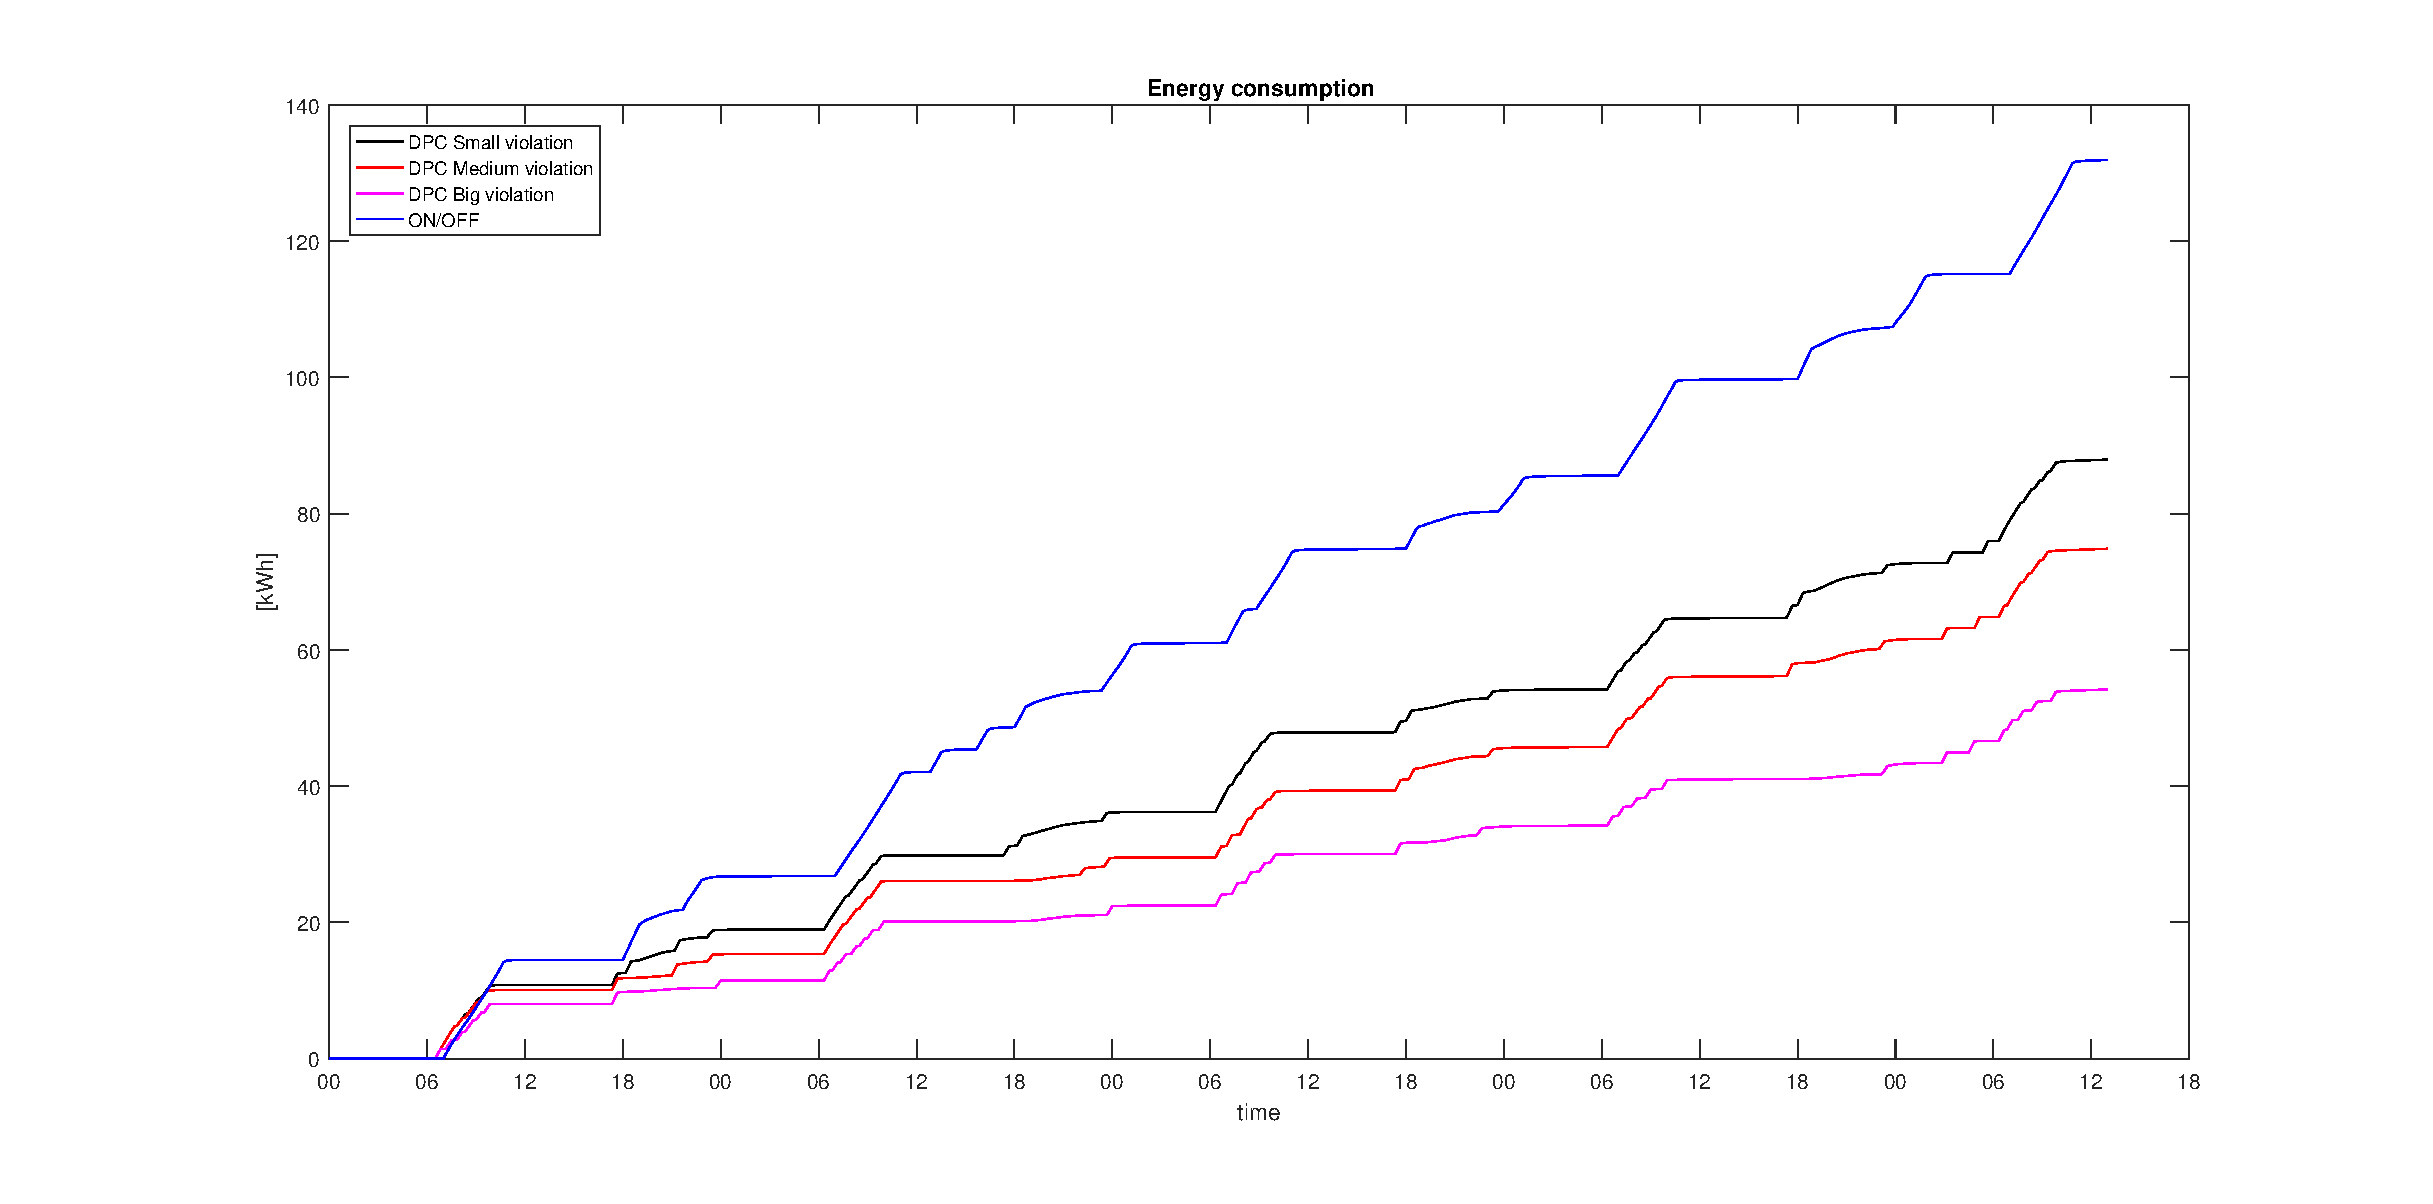
\includegraphics[width=26pc]{figures/Energy_all.eps}
%	\end{center}
%	\caption{Comparison of DPC and bang-bang control performance with different violations using random forest model.}
%	\label{F:comparison_all_energy}
%\end{figure}
%An alternative comparison can be done considering the EnergyPlus model of the house for energy consumption described in Section \ref{SS:energyPlusmodel}. Results are shown in Figure \ref{F:comparison_all_energy_E+}.
In Figure \ref{F:comparison_all_energy_E+}, using the thermal energy consumption model derived in Section \ref{SS:energyPlusmodel} using EnergyPlus, we show how DPC outperforms the bang-bang controller also in terms of energy consumption and how the bounds violations allow us to save more energy. In this case, since the plot is clear and we are interested in showing energy saving on a long period, we ran the simulations over the whole testing period, i.e. $15$ days of May, from May $1$, $2016$ to May $15$, $2016$. We observe that the energy consumption associated to the bang-bang control strategy is approximately equal to $177\,kWh$. If we want to keep the temperature within a comfort range, only allowing small violations, the use of DPC produce an energy saving of $45\, kWh$, that corresponds to the $25.4\%$ over a period of $15$ days. In case of medium violations get an energy saving of $57\, kWh$, that is $32.2\%$. Instead if we allow a large violation over the same period, the energy saving is of $87\, kWh$, that corresponds to the $49.2\%$.
\begin{figure}[t!]
	\begin{center}
		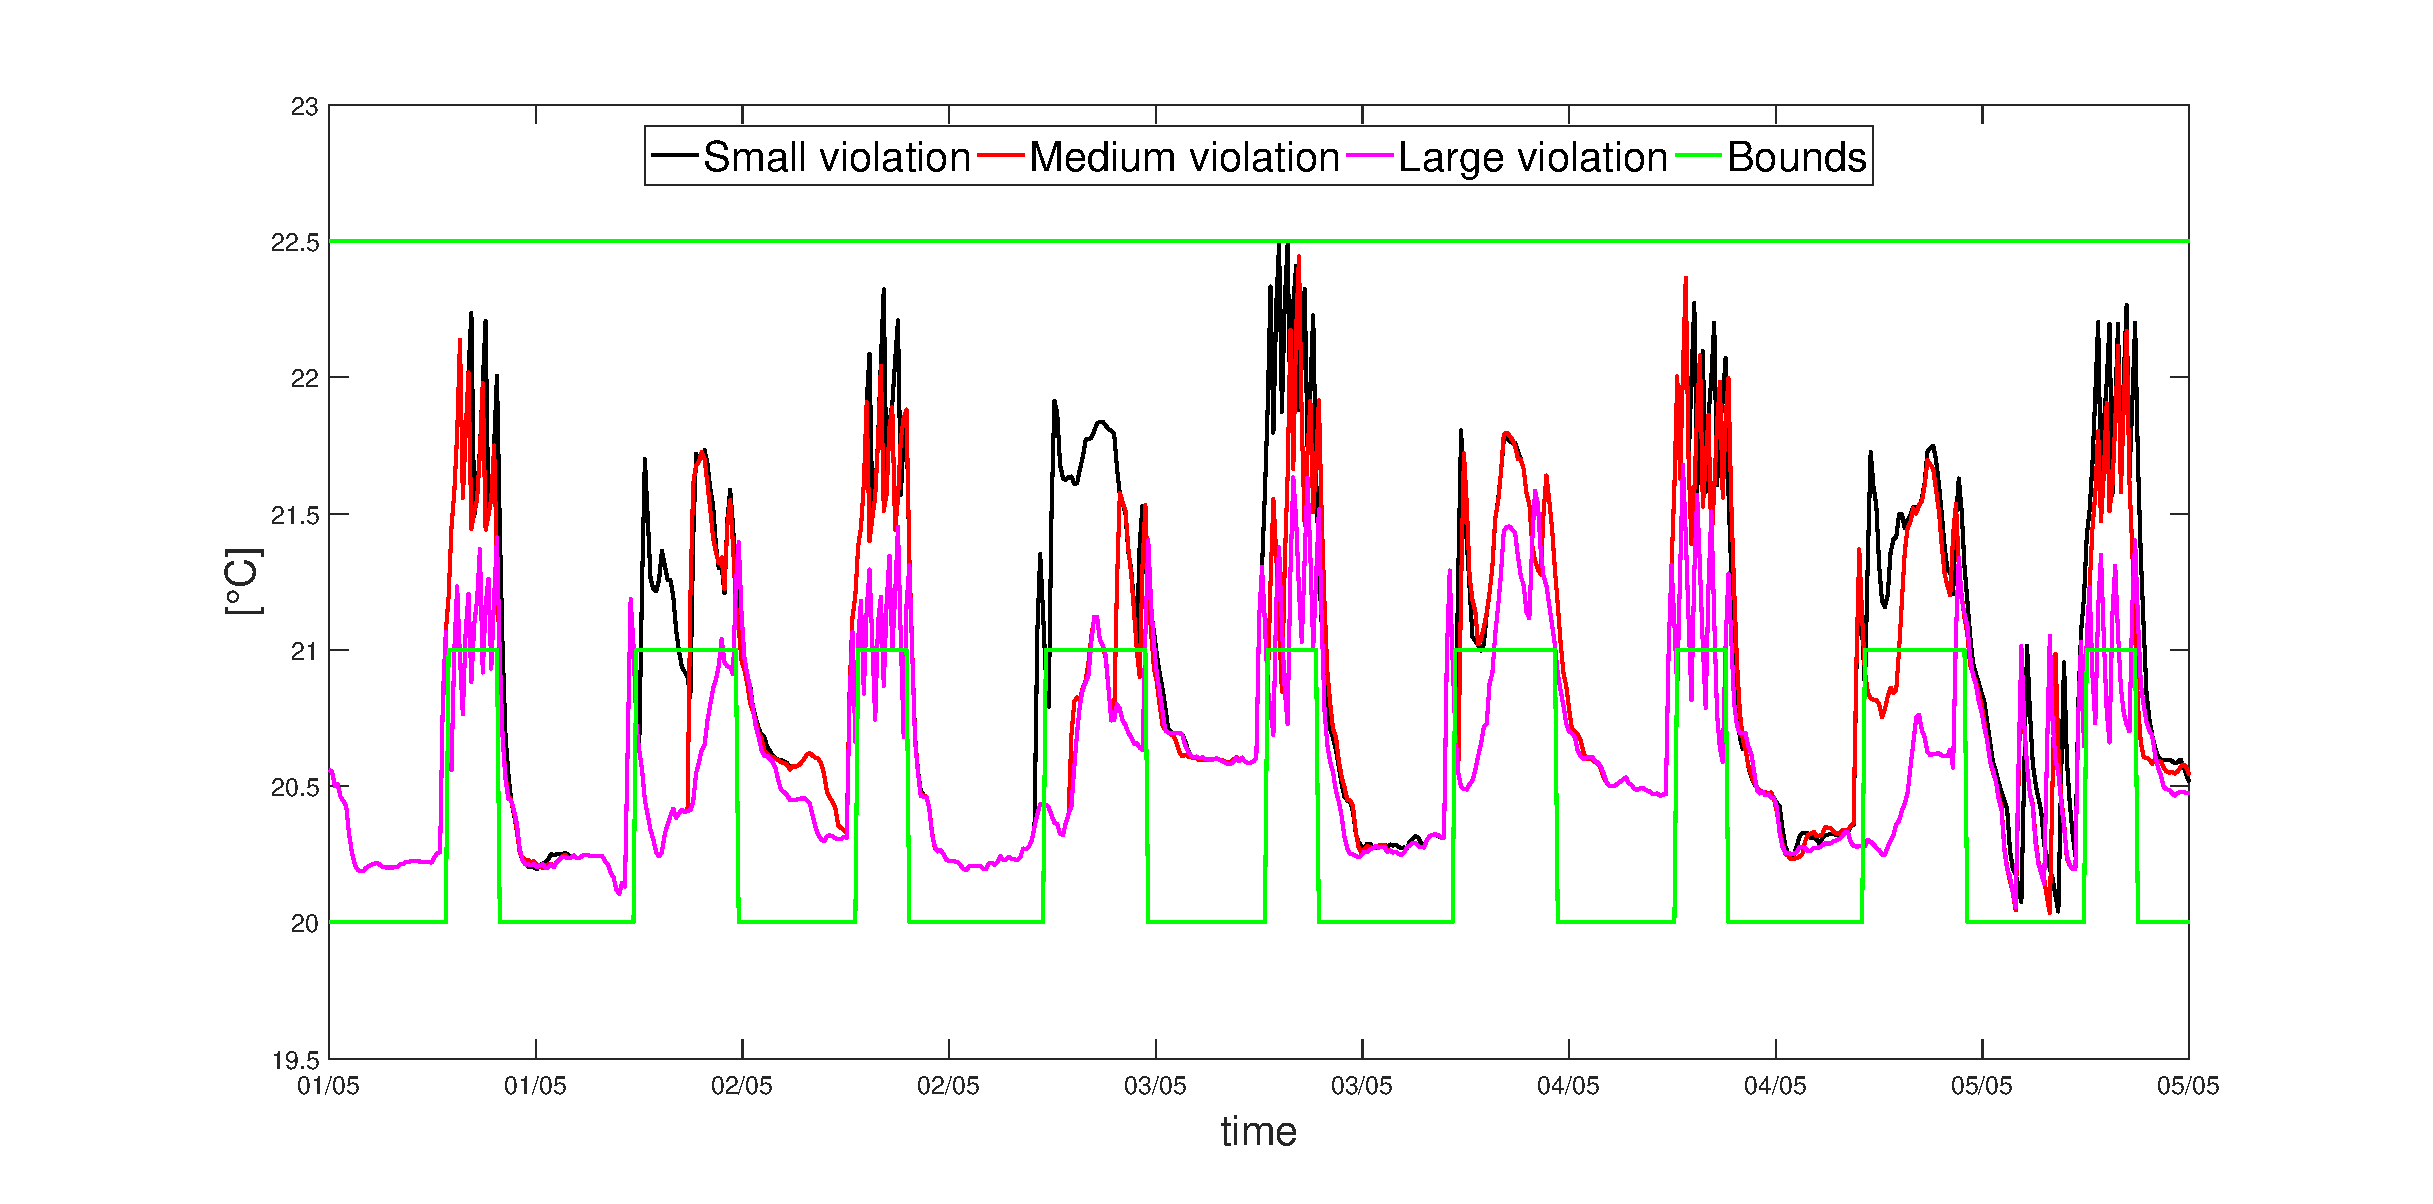
\includegraphics[width=28pc]{figures/Temperatures_all.eps}
	\end{center}
	\caption{Comparison, in terms of comfort, of DPC control performance simulated over $5$ days of the testing period with $3$ different violation configurations: small, medium and large. With the large violation configuration, the temperature is almost always outside of the lower bound when this is tighter. However the maximum bound violation is less than $1\degree C$. With the small violation configuration, the temperature is always within the bound with very few exceptions. However, when it happens, the violation is lower than $0.1\degree C$. The medium violation configuration gives a temperature bound violation that is in the middle with respect to the small and the large ones.}
	\label{F:comparison_all_temperature}
\end{figure}
%\begin{table}[t!]
%	\centering
%	%	\scalebox{0.9}{
%	\begin{tabular}{lccccc}
%		\toprule
%		CONTROLLER  & LBV $\mathrm{MBE}$  & LBV $\mathrm{RMSE}$ & UBV $\mathrm{MBE}$ & UBV $\mathrm{RMSE}$ 	\\ 
%		\midrule
%		$DPC-SV$    & $0.013$             & $0.028$  			      & $0$    				 & $0$     	  	\\
%		$DPC-MV$    & $0.165$ 			  & $0.146$     			  & $0$    				 & $0$		  	\\
%		$DPC-LV$    & $0.410$  			  & $0.224$     			  & $0$    				 & $0$	      	\\
%		$Bang-bang$ & $0.049$ 			  & $0.080$    				  & $0.0063$ 		     & $0.0120$	  	\\
%		\bottomrule
%	\end{tabular}
%	%	}
%	\caption{Lower Bound Violation (LBV) and Upper Bound Violation (UBV) errors expressed as $\mathrm{MBE}\%$ and $\mathrm{CV(RMSE)}\%$ for DPC Small Violation (DPC-SV), DPC Medium Violation (DPC-MV), DPC large Violation (DPC-LV) and bang-bang controller.}
%	\captionsetup{justification=centering}
%	\label{T:violationErrors}
%\end{table}
\begin{table}[t!]
	\centering
	%	\scalebox{0.9}{
	\begin{tabular}{lccccc}
		\toprule
		CONTROLLER  & LBV $\mathrm{MBE}$  & LBV $\mathrm{RMSE}$ & UBV $\mathrm{MBE}$ & UBV $\mathrm{RMSE}$ 	\\ 
		\midrule
		$DPC-SV$    & $0.013$             & $0.092$  			      & $0$    				 & $0$     	  	\\
		$DPC-MV$    & $0.165$ 			  & $0.479$     			  & $0$    				 & $0$		  	\\
		$DPC-LV$    & $0.410$  			  & $0.733$     			  & $0$    				 & $0$	      	\\
		$Bang-bang$ & $0.0485$ 			  & $0.265$    				  & $0.0063$ 		     & $0.040$	  	\\
		\bottomrule
	\end{tabular}
	%	}
	\caption{Lower Bound Violation (LBV) and Upper Bound Violation (UBV) errors expressed as $\mathrm{MBE}\%$ and $\mathrm{CV(RMSE)}\%$ for DPC Small Violation (DPC-SV), DPC Medium Violation (DPC-MV), DPC large Violation (DPC-LV) and bang-bang controller.}
	\captionsetup{justification=centering}
	\label{T:violationErrors}
\end{table}
\begin{figure}[t!]
	\begin{center}
		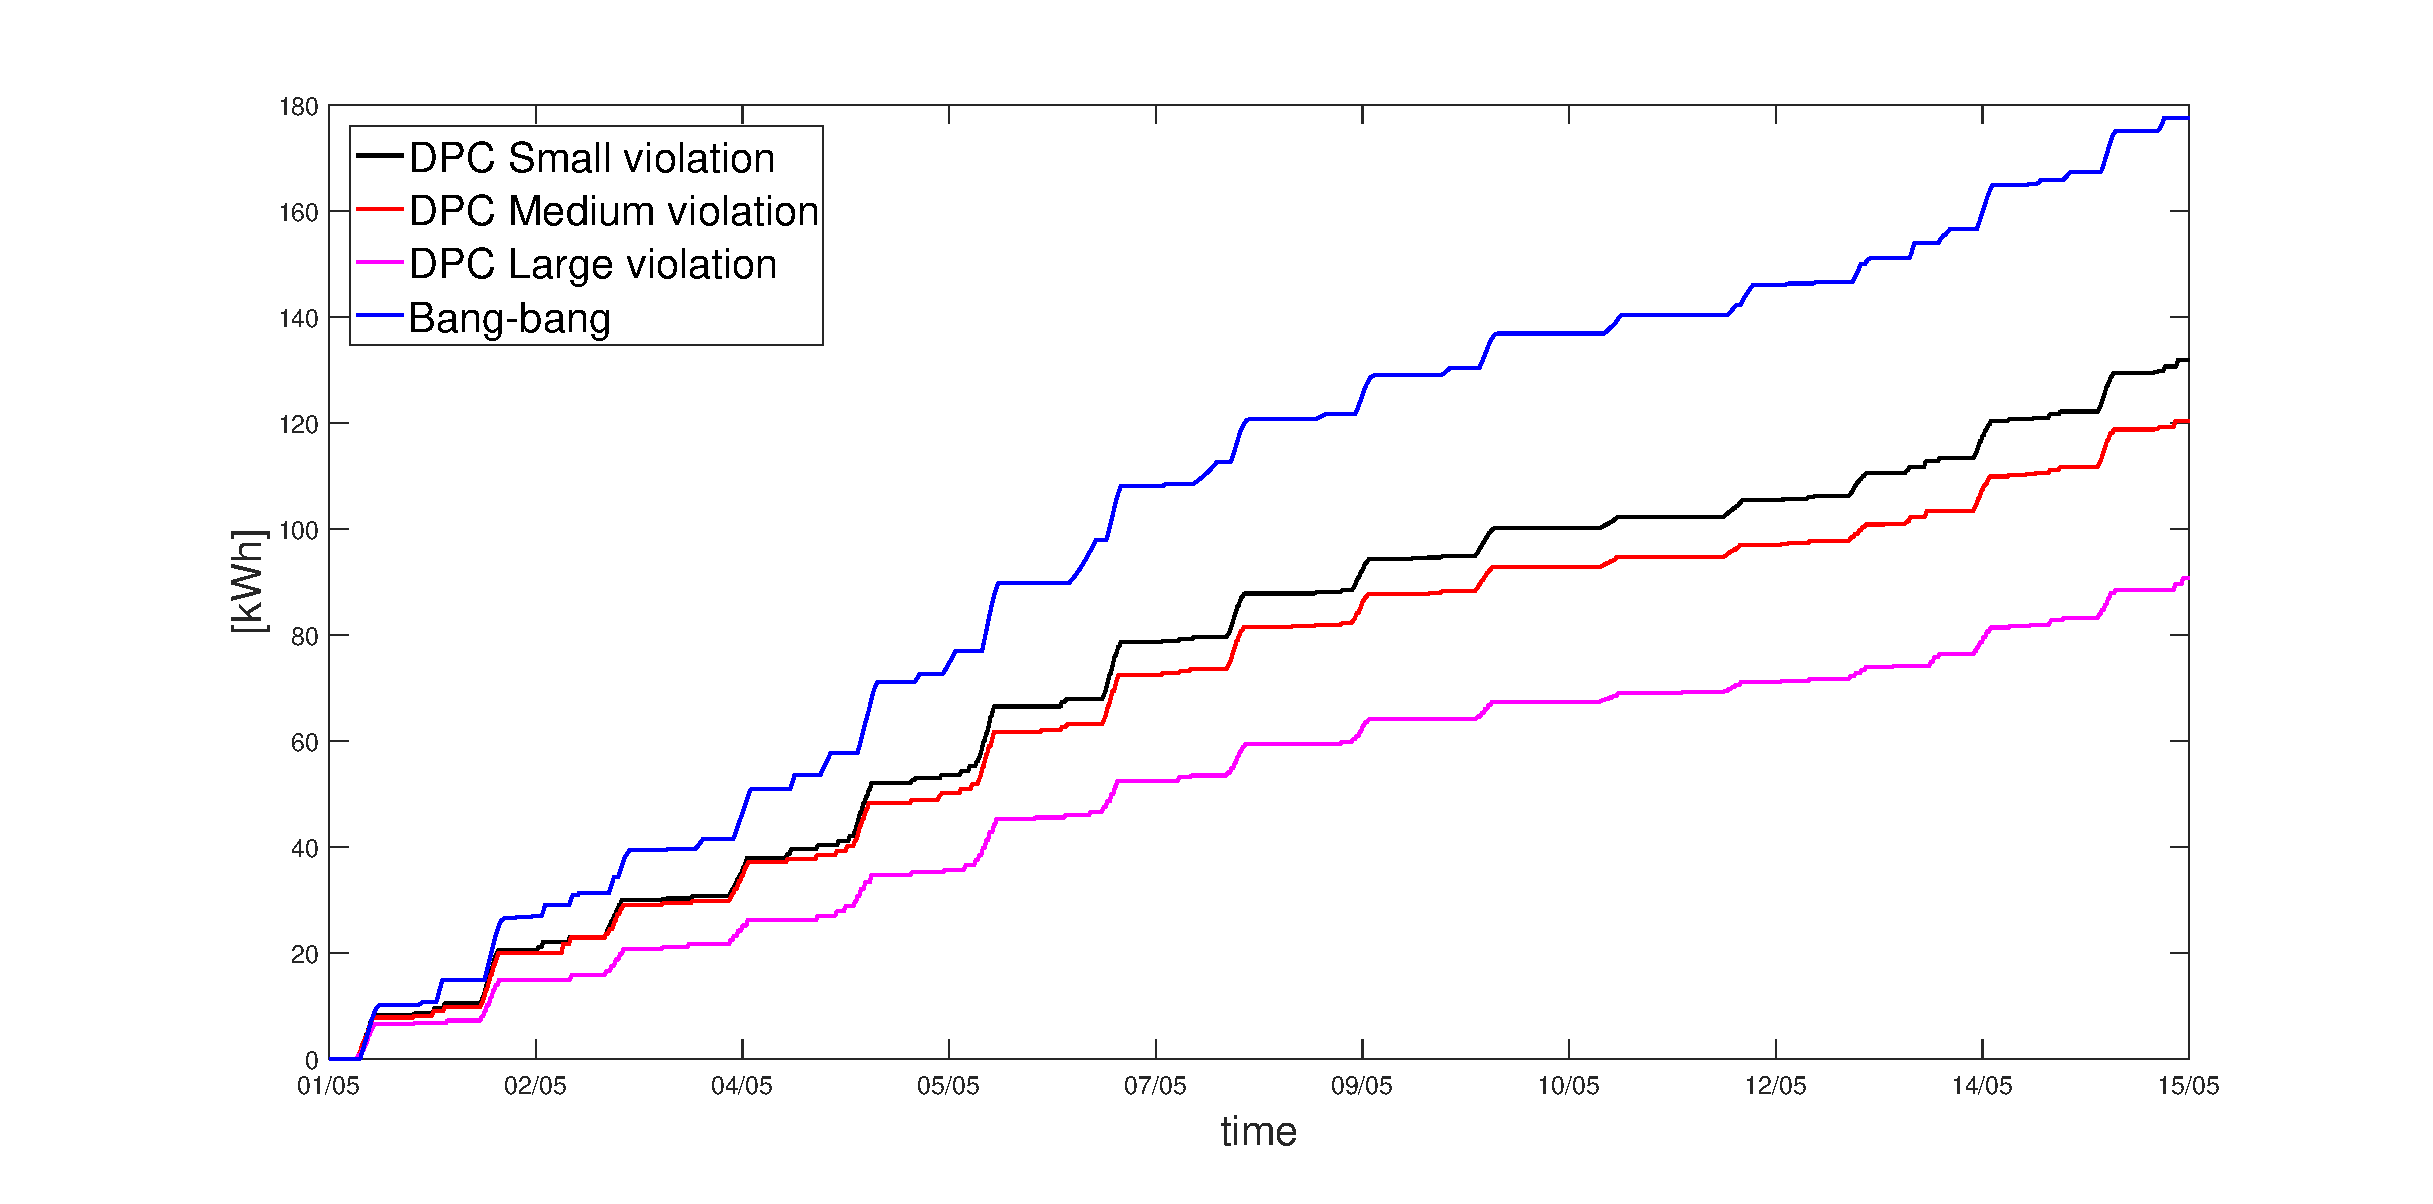
\includegraphics[width=28pc]{figures/Energy_all_EnergyPlus.eps}
	\end{center}
	\caption{Comparison of DPC and bang-bang controller performance over $15$ days of the testing period with different violation configurations, in terms of thermal energy saving using EnergyPlus model. Using bang-bang controller the house energy consumption after $15$ days is of $177kWh$. DPC with small, medium and large violation configurations allows an energy saving of $25.4\%$, $32.3\%$ and $49.2\%$ respectively.}
	\label{F:comparison_all_energy_E+}
\end{figure}

\textcolor[rgb]{0,0,1}{
\subsubsection{Weather forecast subject to uncertainty}\label{SSS:DisturbanceUncertain}
In \cite{Petersen2014AE} the authors investigated, through a large-scale simulation study, the effect of weather forecast uncertainty on the performance of MPC in building systems operations, and compared to the performance of a rule-based strategy.
They considered 48 different scenarios of uncertainties on 72 hours weather forecasts.
On such long horizon, results have shown that, with few exceptions, that MPC outperforms the rule-based controller in case of energy savings and/or thermal indoor environment, and is in general quite close to the perfect forecast case, despite the uncertainty in weather forecast.}

\textcolor[rgb]{0,0,1}{Horizon length for the DPC algorithm presented in this paper is usually much shorter, as for example $6\ hours$ in Section \ref{S:proof}, $7\ hours$ in Section \ref{S:casestudy}, and $40\ minutes$ in Section \ref{S:realCaseStudy}. This means the weather forecast is more accurate than the 72 hours case presented in \cite{Petersen2014AE}, hence also control performance is even closer to the perfect knowledge forecast case.
Nevertheless, to show the robustness of our approach, in this section we provide simulations considering noisy weather forecast.}

\textcolor[rgb]{0,0,1}{To this aim, we add noises with normal distribution on the disturbance variables in $\X^d$, used to obtain parameters $\hat \Theta$ in the DPC problem \eqref{E:DPCrealcase}, i.e. the disturbance in input in the blue rectangle in Figure \ref{F:overview}, while we use the correct ones to simulate the process, i.e. the disturbance in input in the "Plant" box in the red rectangle in Figure \ref{F:overview}.
In Table \ref{T:NoiseParameters} we summarize the mean and the deviation values of the Gaussian noises that we add to each variable.
We obviously do not add any noise on the "Time of the day" and on the "Day of the week" since those are perfectly known.
We considered zero mean since we suppose there is no constant offset in the forecast, but only an error that can over or underestimate the predictions.
In the table, we also report the range of the values that the variables assumed during the reference period of the historical dataset.
This is to show that the deviation values we chose add a quite bad error on the forecast.
In particular, for example, a deviation of $0.5\degree C$ on the outside air temperature means that the error on the predicted temperature lies within the range of $\pm 1.5\degree C$ with a probability of $99\%$.
We solved DPC problem \ref{P:dpcRealCase} considering the new parameters $\hat \Theta$, obtained using the aforementioned noisy forecast, obtaining the following results, where we show the change in performance on bounds violation and energy consumption due to the forecast inaccuracy.}
\begin{table}[t!]
	\centering	
	\textcolor[rgb]{0,0,1}{\begin{tabular}{lccc}
		\toprule
		Variable               & Range      & Mean & Deviation \\ 
		\midrule
		Outside temperature    & [0,31]     & 0	   & 0.5       \\
		Wind                   & [0,5] 		& 0    & 0.25      \\
		Atmospheric pressure   & [990,1030] & 0    & 50        \\
		Relative Humidity      & [20,91]	& 0    & 5         \\
		Solar Radiation        & [0,1000]   & 0    & 50        \\
		Time of the day        & [0,23]     & 0    & 0         \\
		Day of the week        & [1,7]      & 0    & 0         \\
		\bottomrule
	\end{tabular}}
	\caption{\textcolor[rgb]{0,0,1}{Mean and deviation values of the Gaussian noises added on the weather forecast data, and the range of variation of the variables in the historical dataset.}}
	\captionsetup{justification=centering}
	\label{T:NoiseParameters}
\end{table}

\textcolor[rgb]{0,0,1}{\paragraph{Result 1} In Figure \ref{F:ComparisonTempNoisy} a comparison of the DPC results in terms of temperature control for thermal comfort, between the perfect and the noisy forecast, is shown.
We ran the simulations over a period of 15 days, howeveror the sake of plot's clarity, we show only 4 days and a half as simulative period and we split the plot into 3 sub-figures referring to the small, medium and large violation cases.
We can see that in the case of small and large violation we have a small deterioration in performance in terms of bounds violation, although this is more highlighted in the large violation case.
The medium violation cases are instead comparable.
The maximum violation, as in the case of perfect forecast, is still lower than $1\,\degree C$.
In particular, we report in Table \ref{T:violationErrorsNoisy} the violation errors in terms of MBE and CV(RMSE).
If we compare them with the ones in Table \ref{T:violationErrors}, we can see that the performance of DPC with noisy forecast are still good if compared with the performance of DPC with perfect forecast, despite the extremely bad prediction error that we considered on the weather forecast.
}
\begin{figure}[t!]
	\begin{center}
		\vspace{1.1cm}
		\subfigure{
			\label{F:SmallNoisy}
			\centering
			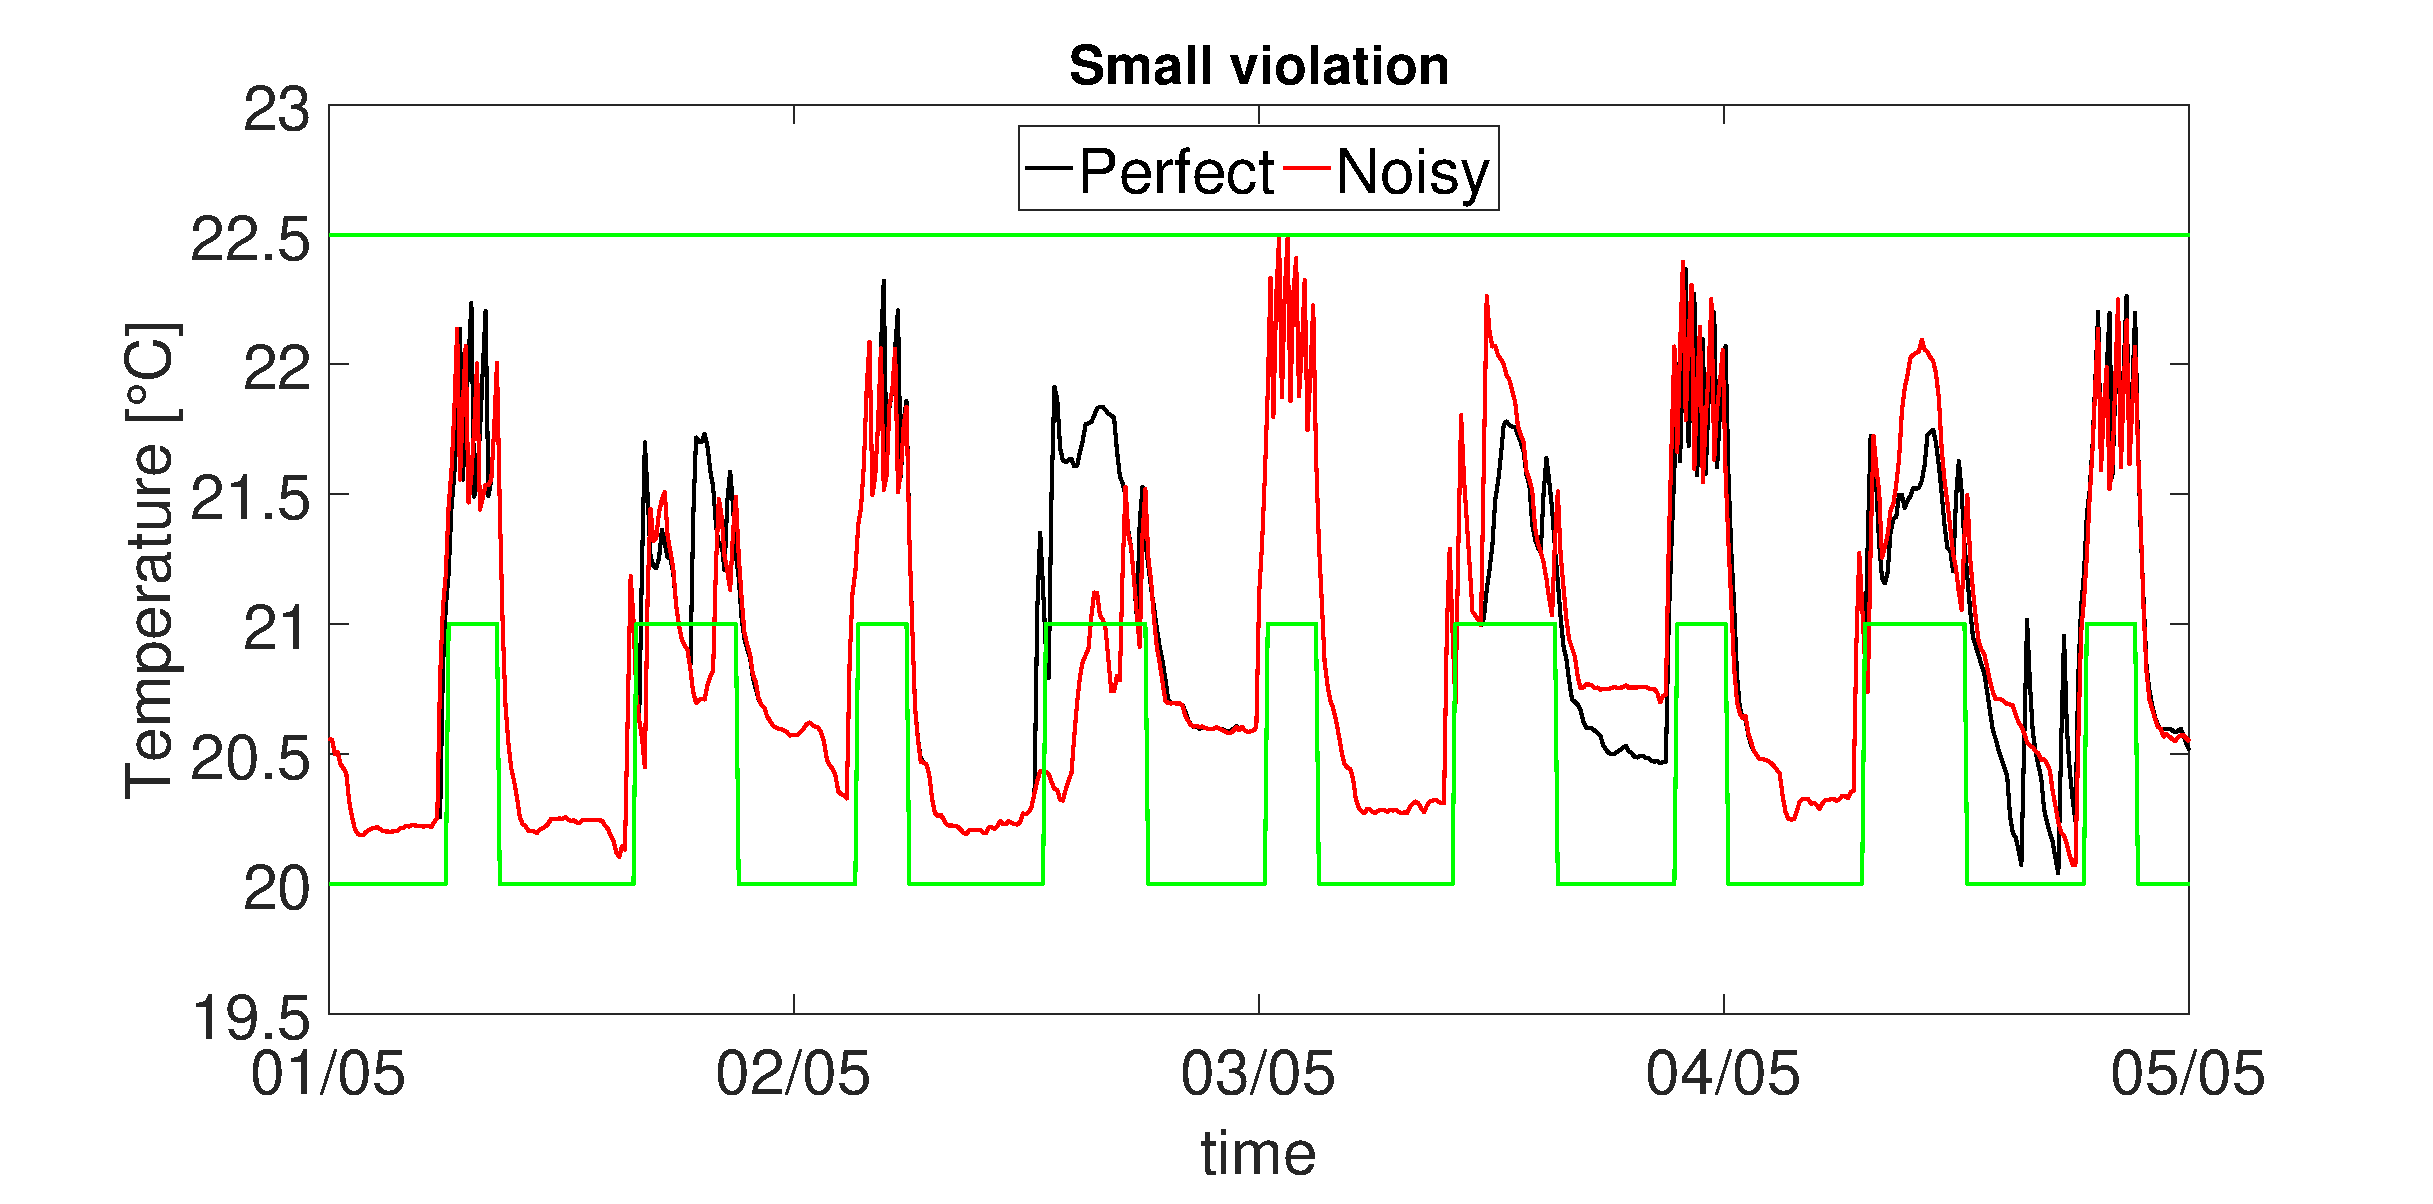
\includegraphics[width=23pc]{figures/Temperatures_small_noisy.eps}
		}	
		\subfigure{
			\label{F:MediumNoisy}
			\centering
			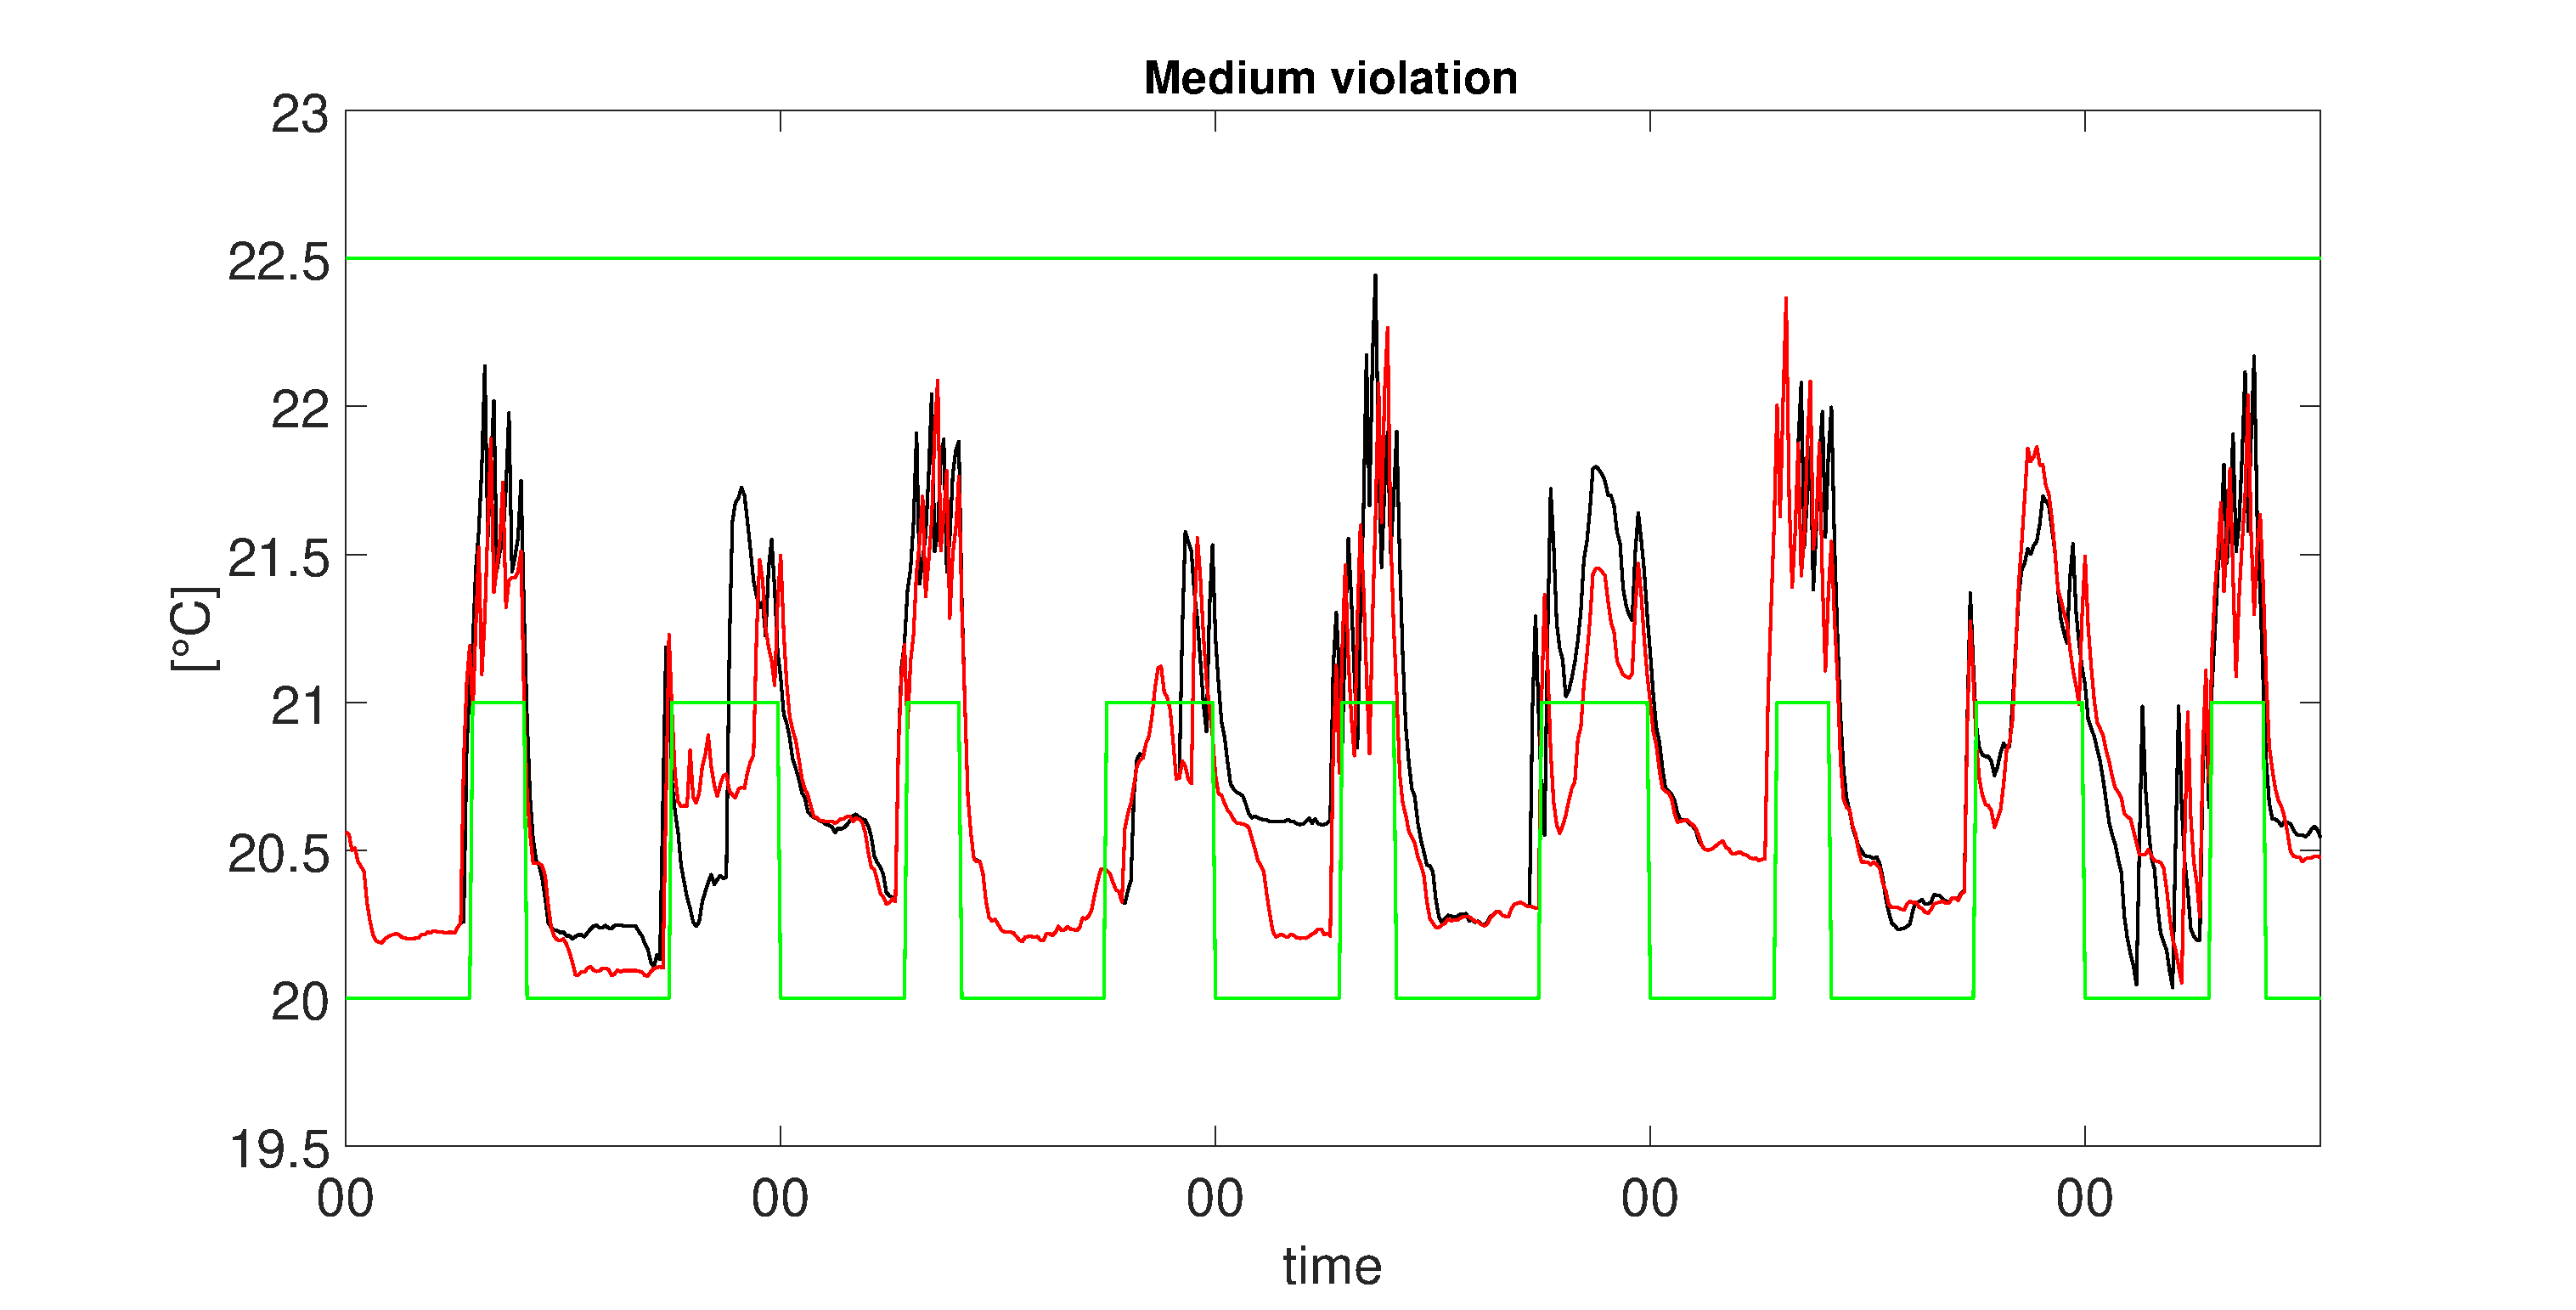
\includegraphics[width=23pc]{figures/Temperatures_medium_noisy.eps}
		}
		\subfigure{
			\label{F:LargeNoisy}
			\centering
			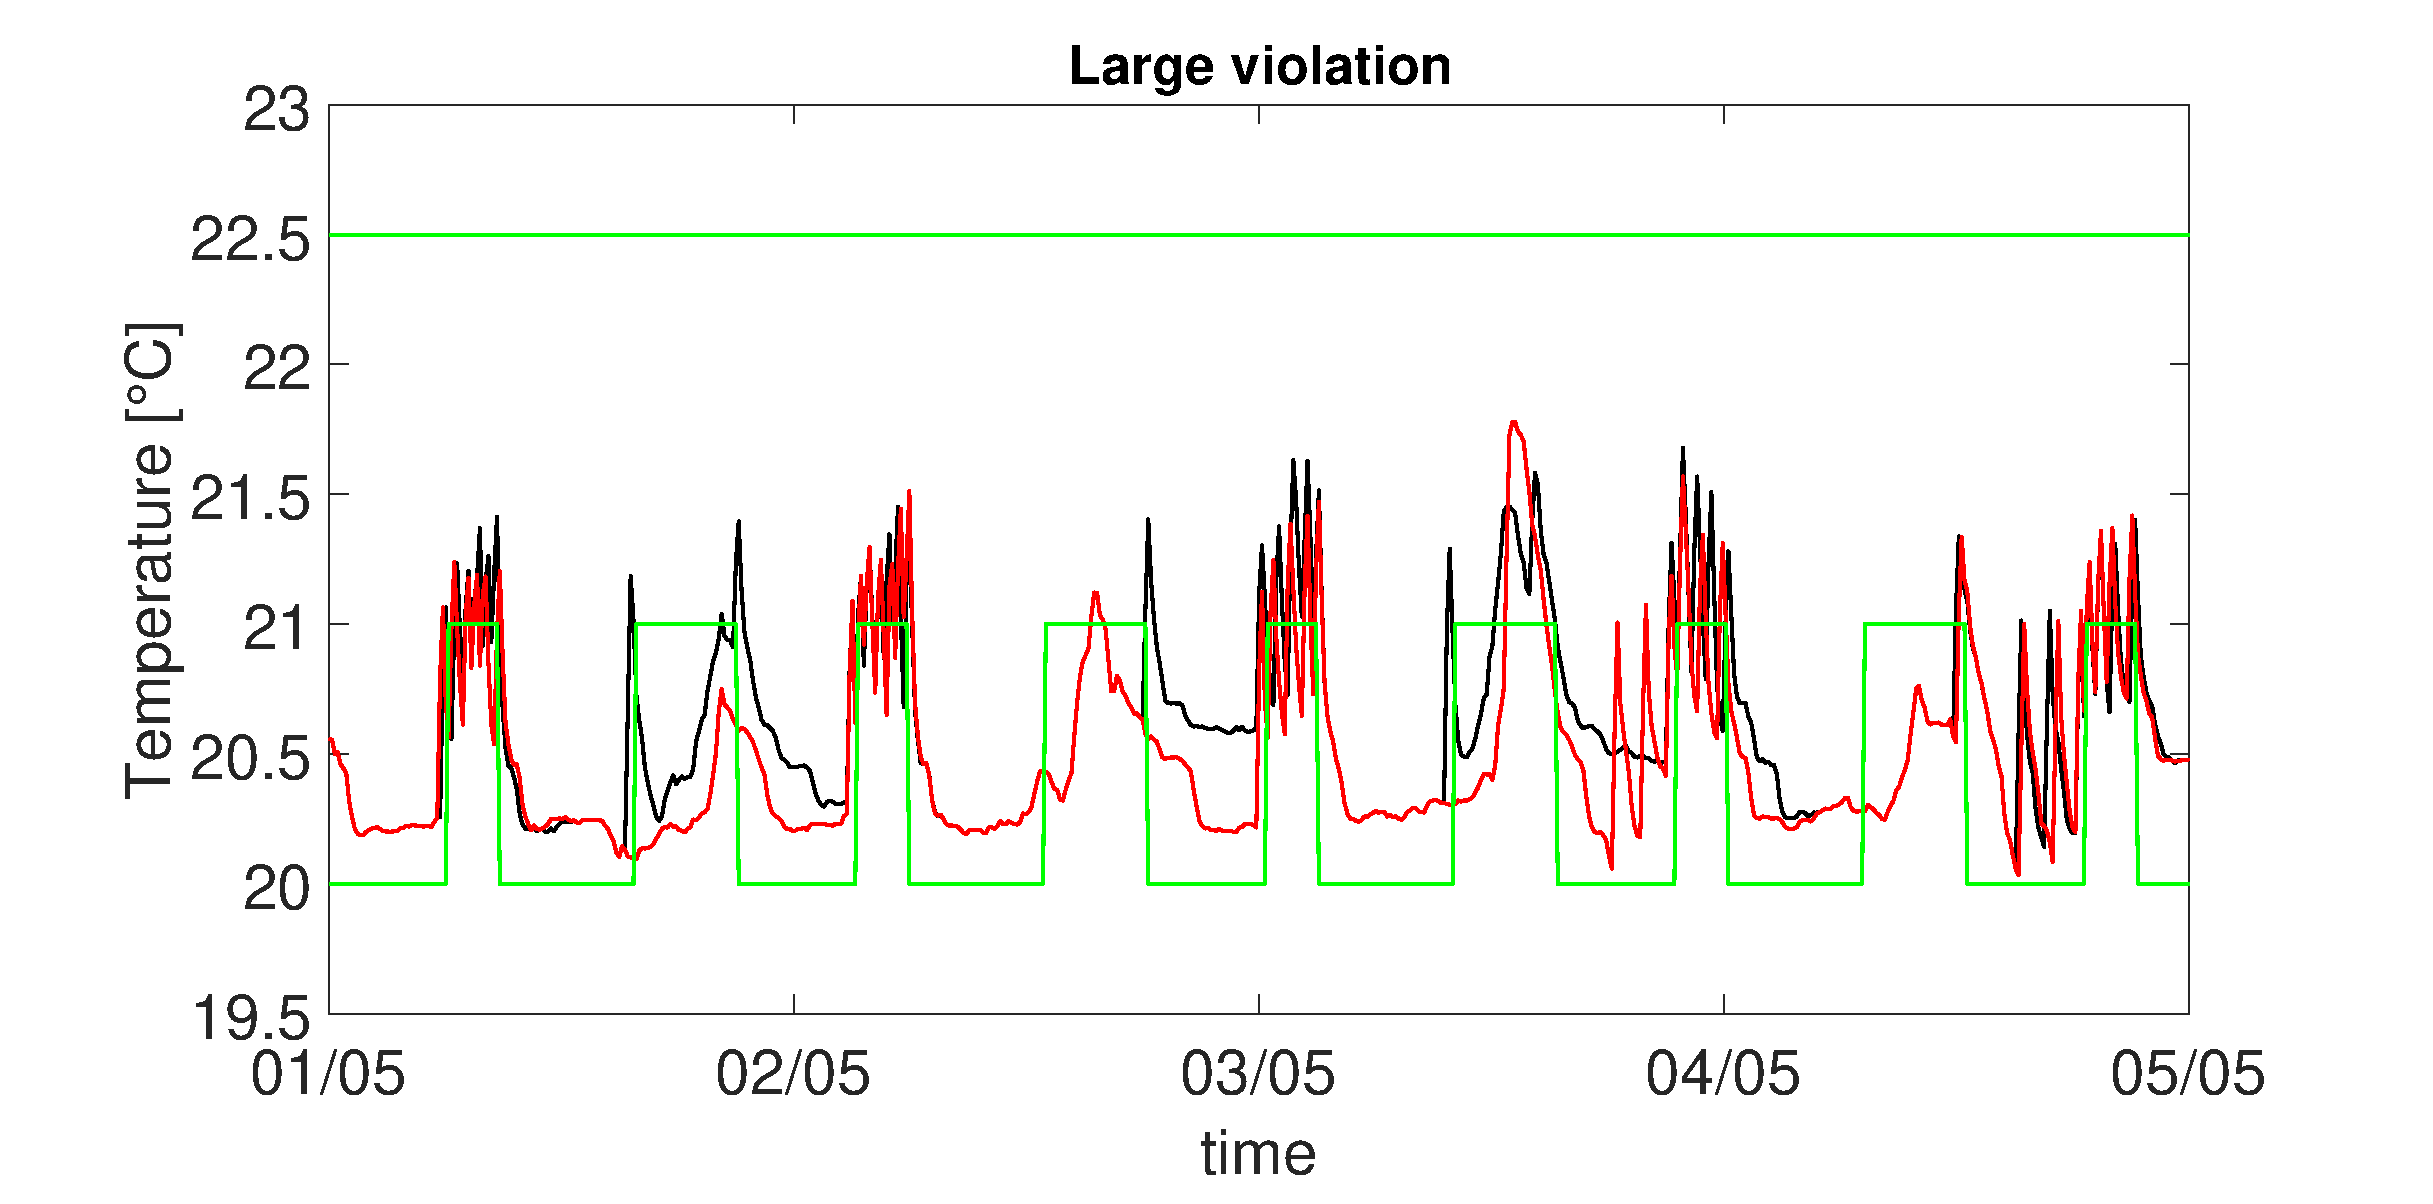
\includegraphics[width=23pc]{figures/Temperatures_large_noisy.eps}
		}	
	\end{center}
	\caption{\textcolor[rgb]{0,0,1}{Comparison of DPC considering perfect and noisy weather forecasts. Small, medium and large violation cases are compared.}}
	\captionsetup{justification=centering}
	\label{F:ComparisonTempNoisy}
\end{figure}

\begin{table}[t!]
	\centering
	%	\scalebox{0.9}{
	\textcolor[rgb]{0,0,1}{\begin{tabular}{lccccc}
		\toprule
		CONTROLLER  & LBV $\mathrm{MBE}$  & LBV $\mathrm{RMSE}$ & UBV $\mathrm{MBE}$ & UBV $\mathrm{RMSE}$ 	\\ 
		\midrule
		$DPC-SV$    & $0.034$             & $0.142$  			      & $0$    				 & $0$     	  	\\
		$DPC-MV$    & $0.178$ 			  & $0.453$       			  & $0$    				 & $0$		  	\\
		$DPC-LV$    & $0.478$  			  & $0.891$     			  & $0$    				 & $0$	      	\\
		\bottomrule
	\end{tabular}}
	%	}
	\caption{\textcolor[rgb]{0,0,1}{Lower Bound Violation (LBV) and Upper Bound Violation (UBV) errors expressed as $\mathrm{MBE}\%$ and $\mathrm{CV(RMSE)}\%$ for DPC Small Violation (DPC-SV), DPC Medium Violation (DPC-MV), DPC large Violation (DPC-LV) and bang-bang controller, considering noisy weather forecast.}}
	\captionsetup{justification=centering}
	\label{T:violationErrorsNoisy}
\end{table}


\textcolor[rgb]{0,0,1}{\paragraph{Result 2} 
In Figure \ref{F:comparison_all_energy_E+_noisy}, we show the difference in terms of energy consumption considering the perfect weather forecast and the noisy one.
We can observe the case with imperfect forecast is very close to the perfect forecast case, and depending the conditions for which the disturbance is over or underestimated, we have more or less energy consumption. These results shows the strong robustness of the DPC with respect to errors in the weather forecast.}
\begin{figure}[t!]
	\begin{center}
		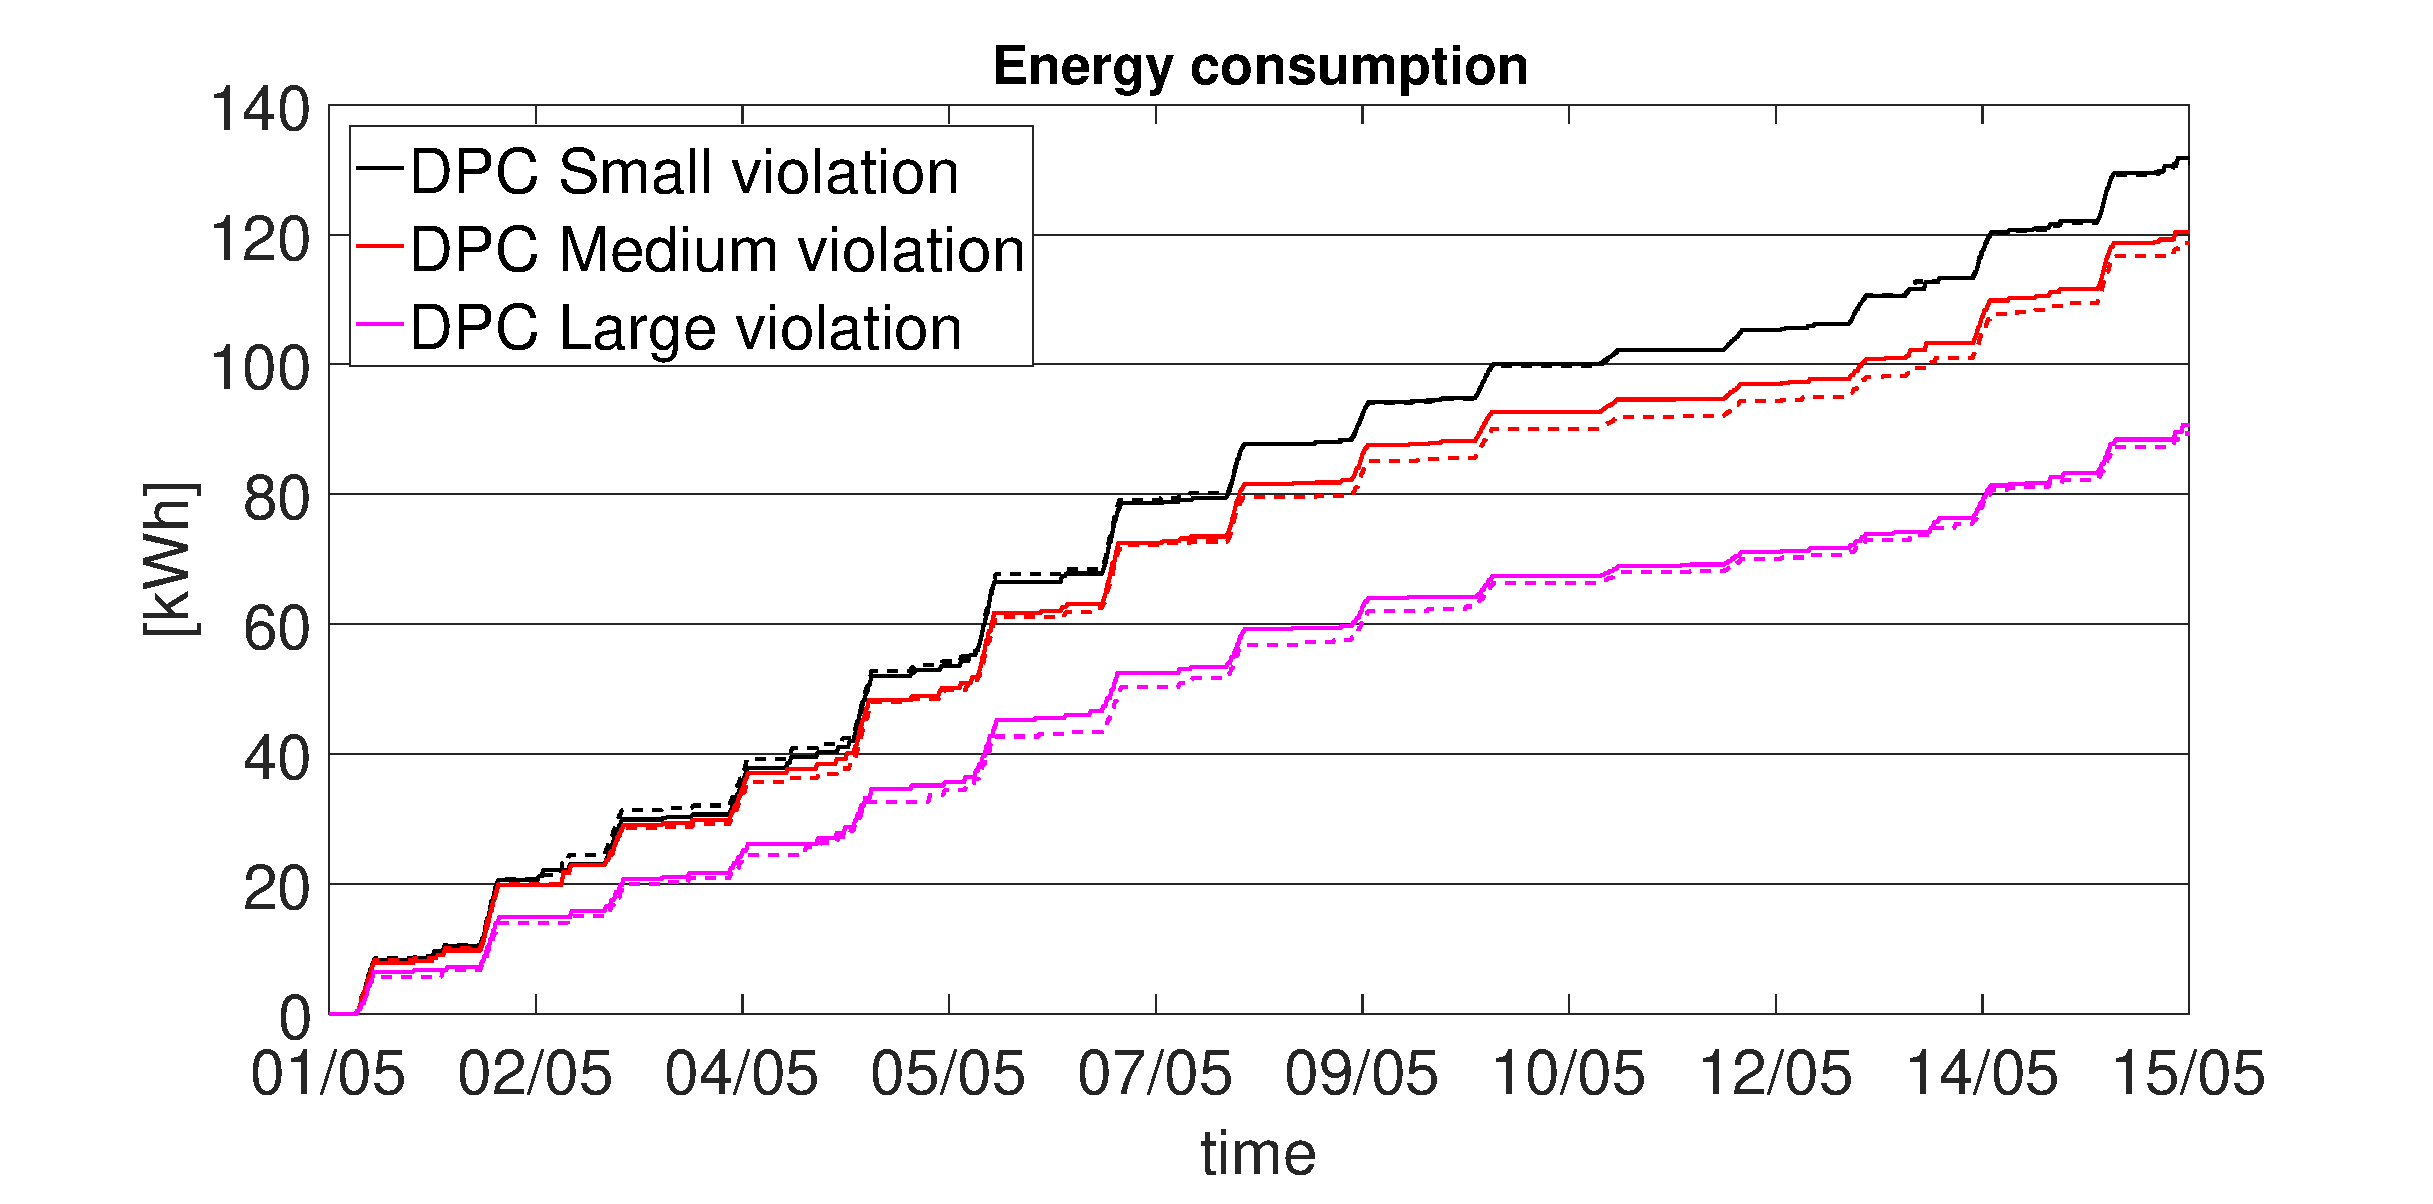
\includegraphics[width=28pc]{figures/Energy_all_EnergyPlus_noisy.eps}
	\end{center}
	\caption{\textcolor[rgb]{0,0,1}{Comparison of DPC in terms of thermal energy saving using EnergyPlus model, considering perfect (full) and imperfect (dashed) weather forecast, over $15$ days of the testing period with different violation configurations. The performance are pretty similar, showing the potential robustness of DPC.}}
	\label{F:comparison_all_energy_E+_noisy}
\end{figure}


%% CONCLUSION
\section{CONCLUSION}
\label{S:conclusion}

To overcome the difficulties associated with the model identification in Model Predictive Control (MPC), we introduce a novel idea for predictive control using data: Data-driven model Predictive Control (DPC). \textcolor[rgb]{0,0,1}{Data-driven control is based on non-physical (black-box) models, therefore they can not be integrated with most of the classical control approaches.} The goal is to create data-driven models that are suitable for receiding horizon control. \textcolor[rgb]{0,0,1}{To this aim, we present two algorithms, based on trees and random forests, to create control-oriented models for DPC. We then apply DPC to three different case studies to demonstrate its strength.}
\begin{enumerate}
\item \emph{\textbf{Comparison with MPC.}} We compare the performance of our DPC to MPC on a multivariable bilinear building model. We establish that DPC with random forests shows a remarkable similarity to MPC in the optimal control strategies explaining $70\%$ variance. On the other hand, DPC with regression trees suffers from practical limitations due to model overfitting.
\item \emph{\textbf{Demand Response application.}} We further apply DPC with random forests to a large scale 6 story EnergyPlus model with 22 zones for which the traditional model-based control is largely unsuitable due to complex dynamics and the cost of model identification. We show that DPC, relying only on the sensor data, can provide significant energy savings while maintaining thermal comfort. Our results demonstrate that even for such complex system, DPC tracks a reference signal with a mean error of $3\%$.
\item \textcolor[rgb]{0,0,1}{\emph{\textbf{Optimal heating system scheduling of a real house.}} We finally apply DPC using experimental data from a real house and compare it with the classical bang-bang controller widely used for temperature control. We show that DPC provides energy savings while guaranteeing thermal comfort for the occupants. With respect to a bang-bang controller, we obtain energy savings that go from $25.4\%$, when we force the temperature to be strictly in a comfort range, to $49.2\%$, if we allow small violations in the thermal comfort level. Furthermore, we demonstrate the robustness of DPC considering uncertainties in the weather forecast.}
\end{enumerate}

DPC has applications which go beyond buildings and energy systems, to industrial process control, and controlling large critical infrastructures like water networks, district heating \& cooling. DPC is immensely valuable in situations where first principles based modeling cost is extremely high.

\subsection{Practical Challenges and Future Work}
\label{SS:challenges}
\textit{Data Availability:} The main practical challenge for DPC lies in the availability of data for training and we require answers to questions like how much data (functional testing) is required, and how should the sampling be done? Therefore, the procedure for optimal experiment design, and model improvement with estimation of variance in predictions is one of the main focus of our ongoing work.

\textit{Stability:} While the buildings are inherently stable, many other applications require stability guarantees. In our ongoing work, we are working towards proving asymptotic stability to origin with DPC-RT and DPC-En by using concept of switched LTI systems. This will make DPC useful for systems with faster dynamics.

\textit{Robustness:} Another direction of work is on handling uncertainties in the DPC framework, namely an extension to Scenario DPC to account for the disturbance uncertainty. This will help us in quantifying the robustness of DPC.


%ACKNOWLEDGMENTS
\section*{ACKNOWLEDGMENT}
The authors would like to thank Xiaojing Zhang, a PostDoctoral Researcher at the University of California, Berkeley for providing the building model, and Manfred Morari for his feedback on DPC.

%% BIBLIOGRAPHY
\section*{References}
\bibliographystyle{elsarticle-num}
\bibliography{fsRefs,achinRefs}

\end{document}